%%%%%%%%%%%%%%%%%%%%%%%%%%%%%%%%%%%%%%%%%%%%%%%%%%%%%%%%%%%%%%%%%%%%%%%%%%%%%%%%%%%%%%%%%%%%%%%%%%%%%
% This template is distributed with ABSOLUTELY NO WARRANTY.
% It serves as a guideline and constitutes a basic structure for a
% thesis/dissertation. The user assumes full responsibility for formatting
% and typesetting their document and for verifying that all the thesis
% requirements set by the University of Tennessee are met. Please refer to the most
% recent UT thesis guide (http://gradschool.utk.edu/thesesdissertations/formatting/)
% or contact the thesis consultant (http://gradschool.utk.edu/thesesdissertations/).
% Please report any bugs to the thesis consultant.
%%%%%%%%%%%%%%%%%%%%%%%%%%%%%%%%%%%%%%%%%%%%%%%%%%%%%%%%%%%%%%%%%%%%%%%%%%%%%%%%%%%%%%%%%%%%%%%%%%%%%
% O P T I O N S:
% 1. thesis/dissertation
% 2. monochrome
% 3. all options provided by the report class
%%%%%%%%%%%%%%%%%%%%%%%%%%%%%%%%%%%%%%%%%%%%%%%%%%%%%%%%%%%%%%%%%%%%%%%%%%%%%%%%%%%%%%%%%%%%%%%%%%%%%
%First, is this a thesis or dissertation? Choose one by commenting out the one you don't need:
%\documentclass[thesis,letterpaper,12pt]{utthesis} % thesis
\documentclass[dissertation,letterpaper,12pt]{utthesis} %dissertation
% some alternatives are:
%\documentclass[thesis,monochrome,letterpaper,12pt]{utthesis} %thesis, monochrome text
\renewcommand{\baselinestretch}{1.5} 	 % line Spacing
%%%%%%%%%%%%%%%%%%%%%%%%%%%%%%%%%%%%%%%%%%%%%%%%%%%%%%%%%%%%%%%%%%%%%%%%%%%%%%%%%%%%%%%%%%%%%%%%%%%%%
% TO DO: FILL IN YOUR INFORMATION BELOW - READ THIS SECTION CAREFULLY
%%%%%%%%%%%%%%%%%%%%%%%%%%%%%%%%%%%%%%%%%%%%%%%%%%%%%%%%%%%%%%%%%%%%%%%%%%%%%%%%%%%%%%%%%%%%%%%%%%%%%
\title{$\beta$-delayed neutron emission spectroscopy in the \textsuperscript{78}Ni region and development of YSO-based implantation detector}	       	% title of thesis/dissertation
\author{Maninder Singh}                			% author's name
\copyrightYear{2021}            				% copyright year of your thesis/dissertation
\graduationMonth{May}           				% month of graduation for your thesis/dissertation
\degree{Doctor of Philosophy}	    			% degree: Doctor of Philosophy, Master of Science, Master of Engineering...
\university{The University  of Tennessee, Knoxville}	% school name
%%%%%%%%%%%%%%%%%%%%%%%%%%%%%%%%%%%%%%%%%%%%%%%%%%%%%%%%%%%%%%%%%%%%%%%%%%%%%%%%%%%%%%%%%%%%%%%%%%%%%
% LOAD SOME USEFUL PACKAGES. 
% No need to change anything here, although if you'd like to add packages you can do that here. Note that packages preloaded with the utthesis class are: amsmath,amsthm,amssymb,setspace,geometry,hyperref,and color
%%%%%%%%%%%%%%%%%%%%%%%%%%%%%%%%%%%%%%%%%%%%%%%%%%%%%%%%%%%%%%%%%%%%%%%%%%%%%%%%%%%%%%%%%%%%%%%%%%%%%
\usepackage{nomencl}                    % produces a nomenclature
\usepackage{float}                      % figure floats
\usepackage[numbers]{natbib}                     % this package allows you to link your references
\usepackage{graphicx}					% graphics package
\graphicspath{ {pictures/}}% specify the path where figures are located
\usepackage{fancyhdr}                   % fancy headers and footers
\usepackage{url}                        % nicely format url breaks
\usepackage[inactive]{srcltx}		 	% necessary to use forward and inverse searching in DVI
\usepackage{relsize}                    % font sizing hierarchy
\usepackage{notoccite}
\usepackage{booktabs}                   % professional looking tables
\usepackage[config, labelfont={bf}]{caption,subfig} % nice sub figures
\usepackage{mathrsfs}                   % additional math scripts
\usepackage[titletoc]{appendix}			% format appendix correctly
\usepackage{pdflscape}					% to produce landscape pages if necessary
%%%%%%%%%%%%%%%%%%%%%%%%%%%%%%%%%%%%%%%%%%%%%%%%%%%%%%%%%%%%%%%%%%%%%%%%%%%%%%%%%%%%%%%%%%%%%%%%%%%%%%
% This section formats landscape pages properly with the correct page number.
% This code is only necessary when landscape pages are needed and can be left alone
%%%%%%%%%%%%%%%%%%%%%%%%%%%%%%%%%%%%%%%%%%%%%%%%%%%%%%%%%%%%%%%%%%%%%%%%%%%%%%%%%%%%%%%%%%%%%%%%%%%%%%

%\fancypagestyle{mylandscape}{
%	\fancyhf{} %Clears the header/footer
%	\fancyfoot{% Footer
%    \makebox[\textwidth][r]{% Right
%      \rlap{\hspace{.75cm}% Push out of margin by \footskip
%        \smash{% Remove vertical height
%          \raisebox{4.87in}{% Raise vertically
%            \rotatebox{90}{\thepage}}}}}}% Rotate counter-clockwise
%  \renewcommand{\headrulewidth}{0pt}% No header rule
%  \renewcommand{\footrulewidth}{0pt}% No footer rule
%}


%%%%%%%%%%%%%%%%%%%%%%%%%%%%%%%%%%%%%%%%%%%%%%%%%%%%%%%%%%%%%%%%%%%%%%%%%%%%%%%%%%%%%%%%%%%%%%%%%%%%%
\begin{document}
    \pagenumbering{alph} % this is needed to clear certain issues with the hyperref package
    %
    \addToPDFBookmarks{0}{Front Matter}{rootNode} % create a root node named "Front Matter" in the pdf bookmarks
    \addToPDFBookmarks{1}{Title}{a} % add a pdf bookmark to the title page
    \makeTitlePage % make the title page.
    %
    \pagenumbering{roman}
    \setcounter{page}{2}
    %
    \makeCopyrightPage % make the copyright page
    %
%%%%%%%%%%%%%%%%%%%%%%%%%%%%%%%%%%%%%%%%%%%%%%%%%%%%%%%%%%%%%%%%%%%%%%%%%%%%%%%%%%%%%%%%%%%%%%%%%%%%%
%The dedication and acknowledgments are optional. If you wish not to include them, simply comment out both the "\addToPDF..." line and the "\include{...}" line for each.
%%%%%%%%%%%%%%%%%%%%%%%%%%%%%%%%%%%%%%%%%%%%%%%%%%%%%%%%%%%%%%%%%%%%%%%%%%%%%%%%%%%%%%%%%%%%%%%%%%%%%
    \addToPDFBookmarks{1}{Dedication}{b} % add a pdf bookmark to the dedication page
    \chapter*{}
\begin{center}
{\centering \it dedication... }
\end{center}  % include the dedication

    \addToPDFBookmarks{1}{Acknowledgments}{c} % add a pdf bookmark to the acknowledgments page
    \chapter*{Acknowledgments}
I would like to thank... % include the acknowledgments
    
    \addToPDFBookmarks{1}{Abstract}{e} % add a pdf bookmark to the abstract page
    \chapter*{Abstract}\label{ch:abstract}
 $\beta$-decay studies of nuclei in the neutron-rich region and far from the valley of stability are vital to understanding nuclear structure evolution and r-process nucleosynthesis. $\beta$-decay strength functions, delayed neutron emission probabilities ($P\textsubscript{n,2n}$) and energy spectra of delayed neutrons are some of the main indicators of the structural complexities of these nuclei, and act as valuable information for simulating r-process pathways. A few facilities around the world are capable of synthesizing nuclei in the \textit{terra incognita} region of the nuclei chart and lying on the r-process pathway. These fragmentation facilities are capable of providing a number of isotopes to study at the same time, requiring a proper identification system to tag these nuclei with atomic mass (Z) and mass-to-charge (A/Q) ratio using heavy-magnet and energy-degrader settings. For the sake of decay studies, a segmented scintillator YSO (Y\textsubscript{2}SiO\textsubscript{5}:Ce doped) based implantation detector was developed at the University of Tennessee, Knoxville. The detector is compact in structure and offers good spatial and timing resolution, crucial for ion-$\beta$ correlations and time-of-flight (ToF) based $\beta$-delayed neutron emission spectroscopy, respectively. The detector was employed as a part of the BRIKEN neutron counter at Radioactive Ion Beam Factory (RIBF) at RIKEN Nishina Center in Japan, aiming to measure $P_{n,2n}$ for nuclei around the {\textsuperscript{78}Ni} region. Another variant of the detector having a more advanced design was used along with VANDLE (Versatile Array for Neutron Detection at Low Energy) to conduct spectroscopy of $\beta$-delayed neutrons in the same region. In this experiment, a direct measurement of energy spectra will provide information about Gamow-Teller strength distributions. It will also directly verify the conclusions from the BRIKEN experiment where evidence for dominating single-neutron emission from two-neutron unbound states is seen in \textsuperscript{84-87}Ga isotopes. % your abstract
    
    \addToPDFBookmarks{0}{Table of Contents}{f}
    \tableofcontents % generate a table of contents
    \listoftables % generate a list of tables
    \listoffigures % generate a list of figures
   
    \newpage
    \pagenumbering{arabic}
    \setcounter{page}{1}
    %%%%%%%%%%%%%%%%%%%%%%%%%%%%%%%%%%%%%%%%%%%%%%%%%%%%%%%%%%%%%%%%%%%%%%%%%%%%%%%%%%%%%%%%%%%%%%%%%%%%%
    % INCLUDE THE CHAPTERS STARTING WITH THE NOMENCLATURE IF PRESENT
    %%%%%%%%%%%%%%%%%%%%%%%%%%%%%%%%%%%%%%%%%%%%%%%%%%%%%%%%%%%%%%%%%%%%%%%%%%%%%%%%%%%%%%%%%%%%%%%%%%%%%
    \include{front-matter}  
    \chapter{Introduction} \label{ch:introduction}

\section{Background}
An atomic nucleus consisting of neutrons and protons offers a laboratory to get insight into the nature of interactions lead by strong forces. These interactions are deciding factors for the structural arrangement of the nucleons in the nucleus as well as various decay mechanisms. The well-known decay mechanisms fall under the broad term radioactivity, which includes $\beta$-decay, $\alpha$-decay, $\gamma$-decay, and neutron/proton emission [reference]. A unique decay mechanism bearing a combination ($\beta$-decay and neutron emission) of radioactive decays  is called $\beta$-delayed neutron emission.

$\beta$-delayed neutron emission was first discovered in the context of nuclear fission in 1939 by R.B. Roberts et al. \citep{robert1939}. $\beta$-delayed neutron emission is a process observed in nuclei to the right of the line of stability, and gets more intense for (N/Z) $>>$ 1. Nuclei in this region are neutron-rich and neutron emission is expected to occur as we approach the neutron drip line. With an increase in $\beta$ decay Q-value (Q{\textsubscript{$\beta$}}) when going towards the neutron-rich region of the chart of nuclei, $\beta$\textsuperscript{-}-decay becomes the dominant decay mode. The daughter nucleus formed post $\beta$\textsuperscript{-}-decay is in an excited state and unstable against particle emission. The daughter nuclei, instead of deexciting through $\gamma$-ray emission can emit neutrons. Neutron emission may be the dominant mode of decay when the Q{\textsubscript{$\beta$}} value of the decay exceeds the neutron separation energy (S\textsubscript{n}) close to the neutron driplines. Figure \ref{fig:qb-sn} shows the values of (Q{\textsubscript{$\beta$}}-$S_{n}$) energy window for known nuclei, it keeps increasing as we have more and more neutrons in the system. Further, the populated states in the daughter nuclei can even lie higher than the two-neutron separation energy S\textsubscript{2n} enabling the emission of one or more neutrons.   

\begin{figure}[h]
	\centering
	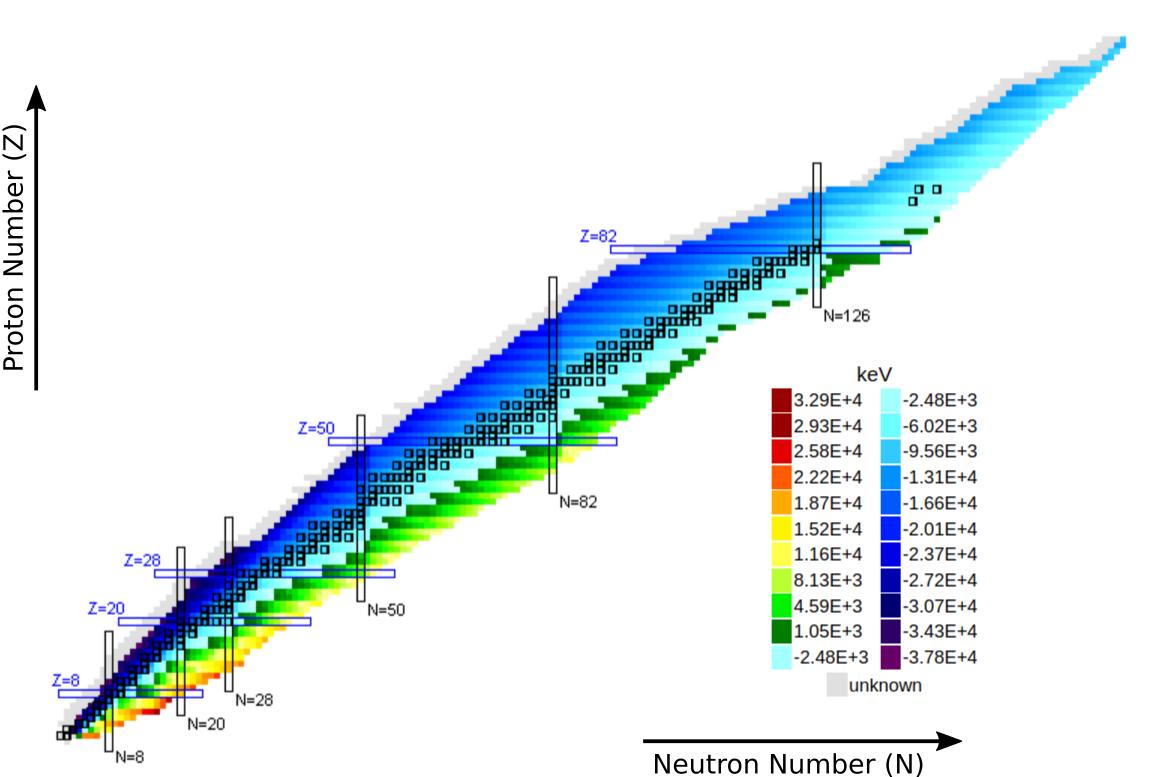
\includegraphics[width=16cm, height=13cm]{figures/Qb_Sn.png}
	\caption[Q{\textsubscript{$\beta$}}-S{\textsubscript{n}} for nuclei in the chart of nuclei..]{Q{\textsubscript{$\beta$}}-S{\textsubscript{n}} for the known isotopes in the nuclear landscape. A higher value is seen for nuclei with large N/Z ratio far-off stability.}
	\label{fig:qb-sn}
\end{figure}  

Over the years, a number of nuclei were seen to exhibit this phenomenon. There are currently just over 200 nuclei with measured emission probability (P\textsubscript{xn}) values. However, a large number of nuclei are expected to engage in beta-delayed neutron emission as suggested by recent work of Moller \textit{et al.,} 2019 \citep{MOLLER20191}, here (P\textsubscript{xn}) values for nuclei spanning the chart of nuclei are predicted. The first observation of multi-neutron emission was seen for \textsuperscript{11}Li and it was identified to be a 2n emitter. $\beta$2n emission is mainly seen in nuclei lighter than Fe ranging from Li to K. \textsuperscript{86}Ga \citep{Yokoyama2018, 86Ga} stands as the strongest 2n emitter to date with measured 2n emission branching ratio of $\sim$ 15\%. \textsuperscript{100}Rb was known to be the heaviest $\beta$2n emitter with P\textsubscript{2n} value equal to 0.16(8)\%. Recent measurements for nuclei in A $\geq$ 100 have resulted in identifying \textsuperscript{136}Sb as a 2n emitter with a small P\textsubscript{2n} value of 0.14(13)\%. Three-neutron emission is theoretically predicted in the A$\geq$100 region of the nuclei chart \citep{MOLLER20191} but has never been experimentally measured. The P\textsubscript{1n} values are scarce for nuclei in the heavy mass region A$\geq$ 150 and no P\textsubscript{2n,3n} are known above mass A=100. 




Study of delayed neutrons is essential to a variety of fields ranging from nuclear structure and astrophysics to nuclear energy. With the advancement in the beam facilities enabling synthesis of nuclei in the \textit{terra incognito} region, coupled with advanced detectors and electronics, the study of such exotic nuclei is now possible. The $\beta$-decay properties of these radioactive isotopes give valuable information on nuclear structure/shell evolution in the regions far-off stability and provide input for astrophysical nucleosynthesis calculations. Several studies show peculiar structural aspects of nuclei solely from measured T\textsubscript{1/2} and P\textsubscript{n} values. One of these studies have hinted at single-particle structures and deformations in the ground state of Sr isotopes, mainly in the region 50$\leq$ N $\leq$ 60. Using $\beta$-delayed neutron emission branching ratios, $\beta$-decay strength distribution ($S_{\beta}$(E)) can be measured. Shifts in the value of $S_{\beta}$(E) have been linked to large deformations in \textsuperscript{42}Si \citep{n28}. Delayed neutron emission spectroscopy of \textsuperscript{83,84}Ga \citep{78Nimiguelmadurga} using VANDLE \citep{VANDLE} has revealed a prevalent mechanism of beta-delayed neutron emission in nuclei far from stability, giving strong evidence in support of Gamow-Teller transition, pertaining to large $S_{\beta}$(E) above the neutron-separation energy. Measurements on \textsuperscript{83,84}Ga also suggest \textsuperscript{78}Ni core excitation, leading to high neutron-emission branching ratios.

 

The $\beta$n-emission probabilities contain information about the structure of involved states and their energy differences. For the medium and heavy nuclei, the $P_{n}$ values show sensitivity to the competition between allowed Gamow-Teller(GT) and first-forbidden(FF) $\beta$-transitions caused by the ordering of the single-particle shell model states. The data regarding delayed-neutron branching ratios are also helpful to test the robustness of nuclear structure models far-off stability. The nuclei at and around shell gaps, e.g., in the doubly magic \textsuperscript{78}Ni region, are an excellent testing and development ground for a variety of physical models. Many of the r-process \citep{burdbidge}  nuclei are expected to be $\beta$-delayed two-neutron emitters, but the competition between $\beta$1n and $\beta$2n decay modes is not understood yet. The quantitative modeling of this effect requires the knowledge of the $\beta$-strength distribution, as well as a statistical model treatment of the competition between one- and two-neutron emission from the excited states in the daughter nucleus. The experiments include the direct $\beta$n branching ratio measurement in the decay of \textsuperscript{78}Ni$\textendash$the only particle-bound doubly-magic nucleus emitting $\beta$-delayed neutrons. A competition between one- and two-neutron emission has been hinted by Miernik \textit{et al.} \citep{86Ga} in the study of \textsuperscript{86}Ga. Results from the experiments at RIKEN are consistent with these measurements and bring about the incapability of the shell-model calculations to reproduce the $P_{1n, 2n}$ values. More data points in the region will help test the robustness of these models. The large decay strength deduced from the observed intense neutron emission is a signature of Gamow-Teller transformation. This observation was interpreted as evidence for allowed $\beta$ decay to \textsuperscript{78}Ni core-excited states, leaving the nucleus in the highly excited state because of the N = 50 shell gap. 


Further, there is great interest in $\beta$-delayed neutron-emission branching ratios of neutron-rich nuclei, which influence the final isotopic abundances of heavy isotopes during the late stages of rapid neutron capture r-process. A detailed study on the neutron energy and branching ratios can be a stepping stone to understanding the abundance patterns intensifying around the shell closures. Accurate and precise measurements of $\beta$-delayed neutron precursors are required to help improve nuclear physics inputs to modern r-process simulations with the aim of constraining the astrophysical site of the r-process. Experimental data on neutron-rich isotopes can also guide the development of quantified theoretical models capable of making reliable predictions for all nuclei involved in the r-process. Obtaining the critical experimental data will be part of an iterative process that requires close interaction between experimentalists, nuclear theorists, and astrophysicists.


\subsection{Present work}

The focus of the present work is on the research and development work done to develop a segmented-YSO based implantation detector, and experiment performed to study energy distribution of $\beta$-delayed neutrons in the \textsuperscript{78}Ni region using VANDLE. The YSO detector was used alongside BRIKEN counter at RIBF. A variant of the detector was employed in synchronization with VANDLE for neutron energy measurements.

The focus of the present work is also on the VANDLE experiment performed at the Radioactive Ion Beam Factory (RIBF) present at RIKEN Nishina Center, Japan to measure $\beta$-decay strength distribution from neutron-unbound states for the isotopes in the region. The BigRIPS fragment separator present at the facility was used to filter out the reaction products of the 345 MeV/u  \textsuperscript{238}U with \textsuperscript{9}Be target. The experiment is the first endeavor to conduct such measurements in the region. The measurements from the VANDLE experiment will provide the feeding intensity from the excited states in the daughter nucleus, and compute the associated strength with those states.
The dissertation also contains the study of $\beta$-decay of neutron-rich $\textsuperscript{79,80,81}$Cu isotopes decay and comparison with shell-model calculations. 




\section{$\beta$-decay}
The $\beta$-radioactivity was discovered as one component of the natural radioactivity (with $\alpha$ and $\gamma$ components) in the turn of the 20th century. The first experimental observations of this process were electrons emitted from radioactive sources. Further studies showed that the electron energy spectrum was continuous, and that $\beta$-decay seemed to violate conservation laws of nuclear physics (in particular energy, spin, and parity). The experimental observations convinced W. Pauli in 1930 to propose the emission of a second particle simultaneously with the electron, with negligible mass, no electrical charge, spin 1/2 and positive parity. This particle was called later the neutrino, and its experimental evidence was achieved in 1956. 
$\beta$-decay in general described as a process where a nucleus having Z protons and N neutrons decays to a nucleus having the same mass number A but with (Z $\pm$1, $N\mp$ 1). A $\beta$\textsuperscript{-}-decay may be regarded as the transformation of one of the protons to a neutron, and $\beta$\textsuperscript{+}-decay as that of one of the neutrons to a proton.
\begin{equation}
\textbf{$\beta$\textsuperscript{-} decay}: A(Z,N) \to A(Z + 1, N-1) + e\textsuperscript{-} + \overline{\nu}\textsubscript{e}
\end{equation}

\begin{equation}
\textbf{$\beta$\textsuperscript{+} decay}: A(Z,N) \to A(Z-1 , N+1) + e\textsuperscript{+} + {\nu}\textsubscript{e}
\end{equation}

Electron capture is another possibility where a nucleus captures an atomic electron. This process thereby changes a proton to a neutron and simultaneously causes the emission of an electron neutrino.
\begin{equation}
\textbf{Electron capture}:  e\textsuperscript{-} + A(Z,N) \to A(Z-1 , N+1) +{\nu}\textsubscript{e}
\end{equation}

Electron capture is mainly in competition with $\beta$\textsuperscript{+} decay and its probability is proportional to Z\textsuperscript{3} owing to increased Coulomb field and small electronic radius because of small electronic radius with increasing proton number in atoms.

\textbf{Q value} of a reaction is defined as the difference between the total kinetic energy before and after the reaction. 
\begin{equation}
Q = T\textsubscript{f} - T\textsubscript{i}
\end{equation}

Q values can further be expressed in terms of the atomic mass difference between parent and daughter nucleus. The expressions for Q-value for various decay types are listed as follows: 

\begin{equation}
\beta\textsubscript{-} decay:
Q\textsubscript{$\beta$\textsuperscript{-}} = (M(Z,N)  - M(Z-1,N+1))c\textsuperscript{2}  
\end{equation}

\begin{equation}
\beta\textsubscript{+} decay:
Q\textsubscript{$\beta$\textsuperscript{+}} = (M(Z,N)  - M(Z+1,N-1))c\textsuperscript{2} - 2m\textsubscript{e}c\textsuperscript{2}
\end{equation}

the 2m\textsubscript{e}c\textsuperscript{2} terms are used to compensate for the energy require to create a positron emitted and the atomic electron that must be ejected in going from a neutral atom of \textbf{Z} electrons to one with \textbf{Z-1} electrons
\begin{equation}
Q\textsubscript{EC} = (M(Z,N)  - M(Z+1,N-1))c\textsuperscript{2}-B\textsubscript{e}
\end{equation}
where B\textsubscript{e} is the ionization energy of the captured electron.

Nuclear $\beta$-decay was explained as a process undergoing weak interaction by Enrico Fermi \citep{fermitheory} in 1933. \textbf{Transition rate for $\beta$-decay} can be formulated using the Fermi's golden rule formulation, where a transition rate depends upon the strength of the coupling between the initial and final state of a system and upon the number of ways the transition can happen (i.e., the density of the final states)

\begin{equation}
\lambda = \frac{2\pi}{\hbar}|\langle\phi_{k}(r)|H^{'}|\phi_{o}(r)\rangle|^2\rho(E_{f})
\end{equation}

where $\rho$ (E\textsubscript{f}) is the density of final states and $H^{'}$ is the perturbation instigating the transition with $\phi\textsubscript{k}(r)$ and $\phi\textsubscript{o}(r)$ describing the entire initial and final states of the system, respectively. A formulation to determine the strength and the form is needed. The quantum mechanical problem can be broken into two parts: first to identify the matrix elements involved and second to determine the density of final states.

The initial state is characterized by the properties of the parent nucleus (spin, parity), and we assume it to be at rest. The final state is a combination of three particles, a neutral lepton(neutrino/anti-neutrino), a charged lepton (electron/positron), and the daughter nucleus. Considering all the prior statements the decay rate can be written in the form of an integral.

\begin{equation}
\lambda = \frac{g^2 |M_{fi}|\textsuperscript{2}}{2\pi^3\hbar^7c^3}\int_{0}^{p_{max}} F(Z_{D},p_{e})p_{e}^2(Q-T_{e})^2dp_{e}
\end{equation}

Here $|M_{fi}|^2$ is a nuclear matrix element representing the overlap between the initial and final	
nuclear states, g is the strength parameter, $p_{e}$ is the electron momentum, and $T_{e}$ is the electron kinetic energy. $\beta^{+}$-particles will be repelled by the nucleus, and their energy spectra are shifted to higher energy side while $\beta^{-}$-particles will be attracted and slowed down. These effects are incorporated by implementing the coulomb distorted wave functions and are contained in a spectrum distortion expression called the Fermi function, $F(Z_{D},p_{e})$, where $Z_{D}$ is the atomic number of the daughter nucleus. Equation 9.0 can be written in a simplified way by writing the integration part as $f(Z_{D},p_{e})$, known as Fermi-integral. 

\begin{equation}
\lambda = \frac{g^2 |M_{fi}|\textsuperscript{2} m_{e}^5c^4}{2\pi^3\hbar^7}f(Z_{D},p_{e}) 
\end{equation}

or in terms of the half-life of the parent nucleus, $T_{1/2}$ 

\begin{equation}
fT_{1/2}= \ln2\frac{2\pi^3\hbar^7}{g^2 |M_{fi}|\textsuperscript{2} m_{e}^5c^4}
\end{equation}

The left-hand side of this equation is called the comparative half-life, or \textquotedblleft ft-value\textquotedblright   because this value can be measured in experiments and should only depend on the nuclear matrix element and the $\beta$-decay strength constant. Typical \textit{ft} values vary from $10^{3}$ s to $10^{22}$ s; therefore the base ten logarithm of this value or log-ft is usually given in the literature. 

The spin and parity of the nuclear states involved in the $\beta$-decay process play an important role. They will determine the type of transition corresponding to the decay, either \textit{allowed} transition or \textit{forbidden} transition, and indicate how \textquotedblleft fast\textquotedblright the transition is.

\subsubsection{Allowed Transitions}

The notation J\textsuperscript{$\pi$} is used in the following, where J is the total spin of the nucleus or particle, and $\pi$ is the parity associated to that state.\\ The selection rules for allowed transitions are as follows:
\begin{enumerate}
	\item Leptons  $L_{l}$   $\rightarrow$ 0 (no angular momentum carried by the leptons)
	\item Nucleus $\pi_{i}\pi_{f}$ = +1 (no parity change)
\end{enumerate}

Since the two leptons can couple to a total intrinsic spin S, and given the condition that they don’t carry angular momentum, the change in the total angular momentum of the nucleus is dictated by how the spins of the two leptons emitted couple with each other. When the spins of the leptons are anti-parallel the total spin $\vec{S}_{l}$ = 0, and only $\Delta\vec{J}$ = 0 is possible (which is a singlet state). The corresponding transitions are called \textit{Fermi} transitions or \textit{vector} transitions. On the other hand if the spins of the two leptons are aligned $\vec{S}_{l}$ = 1, leading to $\Delta$J = 0, $\pm$1 (triplet state). This type of transition is called \textit{Gamow-Teller} transitions or \textit{axial} transitions. 
\\

Transitions where the spins of the final and initial states are $J_{f} = J_{i} = 0$  $(0 \to 0)$ are pure Fermi transitions. Alternatively, transitions with $\Delta$J = $\pm$1 are called pure GT transitions. A particular case of Fermi transition occurs when the nucleon involved in the $\beta$-decay process does not change any of its quantum numbers. This corresponds to $0^{+} \to  0^{+}$ transitions, which is experimentally observed near the N = Z region. These transitions are labeled as \textit{super-allowed} and offer a fascinating scenario as transitions are completely independent of strong interactions. 

\subsubsection{Forbidden Transitions}
Forbidden transitions follow at least one of the following selection rules:
\begin{enumerate}
	\item Leptons $\to \vec{L}_{l} > 0$, (angular momentum carried by leptons) or,
	\item Nucleus $\pi_{i}\pi_{f}$ = -1 (change of parity)
\end{enumerate}

These transitions are called forbidden because they are highly suppressed compared to allowed transitions. Since the matrix element is squared in the determination of the decay constant, each unit of l that has to be carried by the leptons will suppress the decay constant by approximately a factor $10^{-4}$ compared to the case with l = 0.

Forbidden transitions are classified into two branches, unique and non-unique, depending on the changes of spin and parity of the nucleus involved in the $\beta$-decay. For unique transitions, it appears that only one matrix element contributes to the transition, whereas in non-unique cases, several matrix elements will be participating. So forbidden transitions can be \textquotedblleft unique first-forbidden,\textquotedblright \textquotedblleft non-unique first-forbidden,\textquotedblright \textquotedblleft unique second-forbidden.\textquotedblright

A range of \textit{log-ft} values is characteristic of the type of transition, being super-allowed, allowed or forbidden.


\section{Delayed Neutron Emission}

There are many techniques used to predict the P\textsubscript{n} values, including phenomenological \citep{Phenomenoliogical}, shell model \citep{shellmodelhalflives}, and macroscopic-microscopic theories \citep{pmollermacroscopic}. Properly designed models help to provide information for nuclei far-off the reach of beam facilities. The predictions from the theory can be tested against the experimental calculations. This may lead to a validation of the theoretical approximations and a scope to improve models is always there, given the discrepancies seen between predicted and measured results. Experimentally calculated P\textsubscript{n} values can be compared with predicted values, providing a basis for fine-tuning the physics involved in these models. This also forms a basis to study the nuclear structure aspects on a microscopic basis. 

$\beta$-delayed neutron emission is mainly theorized as a multistage process consisting of the $\beta$-decay of the precursor (A, Z), which results in feeding the excited states of the emitter nucleus (A, Z+1) followed by the $\gamma$ de-excitation to the ground state or neutron emission to an excited state or to the ground state of the final nucleus (A-1, Z+1), where Z is the atomic number and A is the mass number of the precursor. The modeling scheme can also be broken into various steps to achieve the final delayed neutron energy spectrum or emission probabilities. Estimates of the Q\textsubscript{$\beta$} value is done mostly by using Finite Range Droplet macroscopic model by Moller et al. \citep{FRDMmoller}. Quasi-particle Random Phase Approximation (QRPA) model can be used to calculate the $\beta$-decay matrix elements and subsequent $\beta$-strength functions.  


\begin{figure}[h]
	\centering
	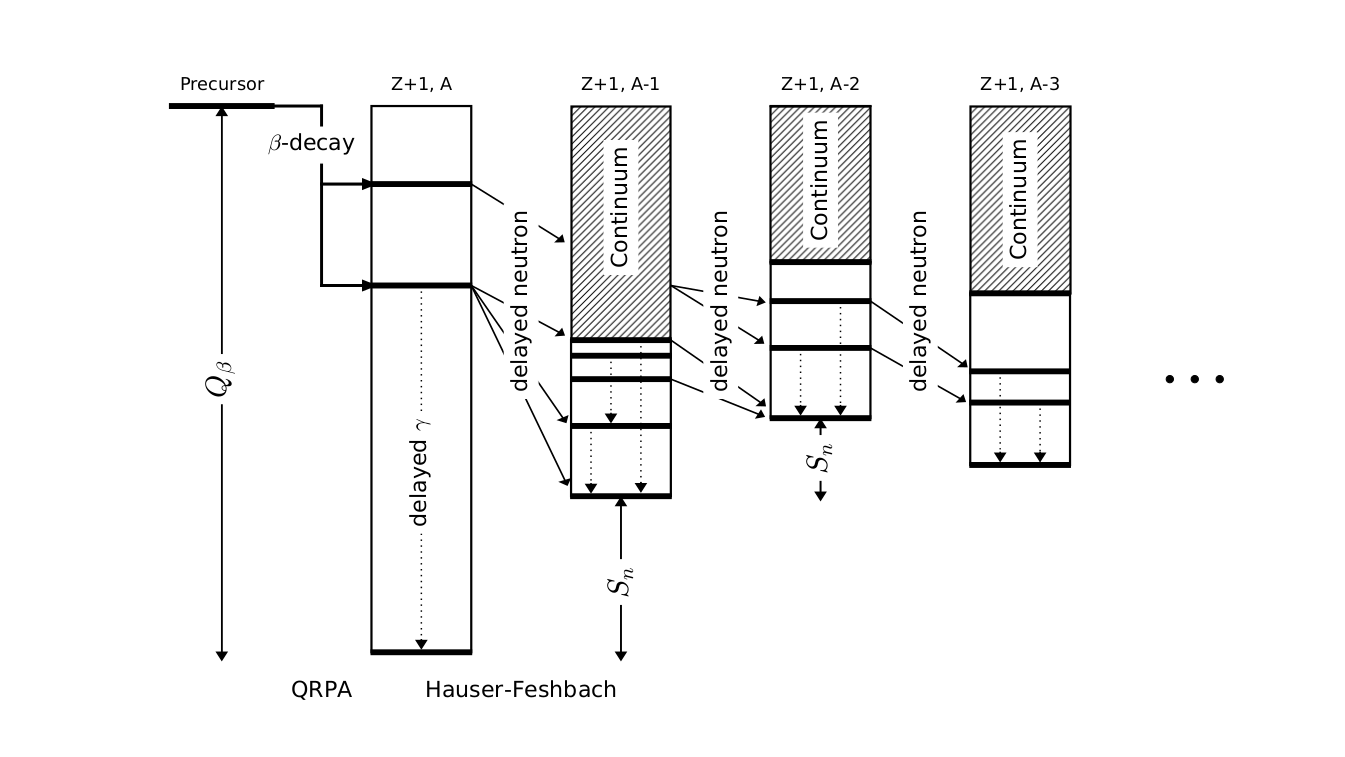
\includegraphics[width=17cm, height=10cm]{figures/delayed_netron_emission_cascaade.png}
	\caption[Schematic of the combined QRPA+HF approach]{Schematic of the combined QRPA+HF approach. Initial population of the the daughter nucleus (Z+1, A) is determined by QRPA. Subsequent delayed neutron and $\gamma$-ray emission are handled in the HF framework and shown by solid and dotted lines respectively. The statistical decay is followed until all available excitation energy is exhausted, denoted by trailing dots \citep{moller2016}. }
\end{figure}

Theoretically, the two integral $\beta$-decay quantities, T\textsubscript{1/2} and P\textsubscript{n}, are intertwined via their definition in terms of the $\beta$-strength function S\textsubscript{$\beta$}(E),

\begin{equation}
1/T_{1/2}=\sum_{0\leq E_{i}\leq Q_{\beta}}S\textsubscript{$\beta$}(E)  \times f(Z,R,Q_{\beta}-E_{i})
\end{equation}
where R is the nuclear radius, $Q_{\beta}$ is the maximum $\beta$-decay energy, and $f(Z,R,Q_{\beta}-E_{i})$ the Fermi function. From this definition, $T_{1/2}$ may contain information about average $\beta$ feeding of a nucleus. However, since transition rates to the low-lying states are strongly enhanced by the phase-space factor of $\beta$-decay, f$\sim (Q_{\beta}- E_{i})^5$, the largest contribution to $T_{1/2}$ comes from decays to the lowest-energy resonances in $S\textsubscript{$\beta$}(E_{i})$; that is, from the (near-) ground state allowed Gamow-Teller (GT) or first-forbidden (ff) transitions.

The $\beta$-delayed neutron emission probability ($P_{n}$) is schematically given by 
\begin{equation}
P_{n}=\frac{\sum_{S_{n}}^{Q_{\beta}} S\textsubscript{$\beta$}(E)\times f(Z,R,Q_{\beta}-E_{i})}{\sum_{0}^{Q_{\beta}} S\textsubscript{$\beta$}(E)\times f(Z,R,Q_{\beta}-E_{i})}
\end{equation}
which defines $P_{n}$ as the ratio of the integral $\beta$ intensity to states above the neutron separation energy, $S_{n}$, to the total $\beta$ intensity. 

The above formulation to get the $P_{n}$ values is mentioned in the literature as '\textit{cutoff}' method. It neglects $\gamma$ competition and assumes that only the higher multiplicity neutron emission prevails in the energy regions open to multiple neutron-emission channels. Also, it ignores the possibility of competition between one- and two-neutron emission as suggested by T. Kawano \textit{et al.,} 2013 \citep{kwano2013}. In order to explain the 1n/2n competition, Mumpower \textit{et al.} \citep{moller2016} implemented Hauser-Feshbach (HF) statistical model with QRPA. This is achieved by first calculating the $\beta$-decay intensities to accessible states in the daughter nucleus using QRPA. The subsequent decay of these states by neutron or $\gamma$-ray emission is then treated in the statistical Hauser-Feshbach (HF) theory. 


\subsubsection{$\beta$-decay feeding intensity $(I_{\beta})$}
When a parent nucleus $\beta$ decays to the daughter nucleus, the occupation of states in the daughter nucleus is controlled mainly by the $\beta$-decay selection rules (wave-function overlaps), i.e, the structure of the parent and the daughter nuclei. The wavefunction overlap between the parent and the daughter states is called the reduced transition matrix element for transitions connecting the states. The energy difference between the states of the parent and the daughter nucleus is another reason, decay to ground state or to states having low energy is preferred. As a general view of the $\beta$ decay, Figure \ref{fig:strength_distribution} shows the decay of a nucleus, and a distribution of S\textsubscript{$\beta$}(E) is shown ranging with the excitation energy in blue. The figure demonstrates the manifestation of equation 1.12 in $\beta$-decay. The low-lying states in the daughter nucleus exhibit a smaller S\textsubscript{$\beta$}(E) due to lesser wavefunction overlap, but S\textsubscript{$\beta$}(E) starts to augment for states above S\textsubscript{n}. The S\textsubscript{$\beta$}(E) can also reach very high values outside the decay window, manifesting as large resonance, known as Gammow-Teller resonance (GTR). The final $(I_{\beta})$ at a given excitation energy is decided by a convolution of S\textsubscript{$\beta$}(E) and phase-space factor at that energy.


\begin{figure}[h]
	\centering
	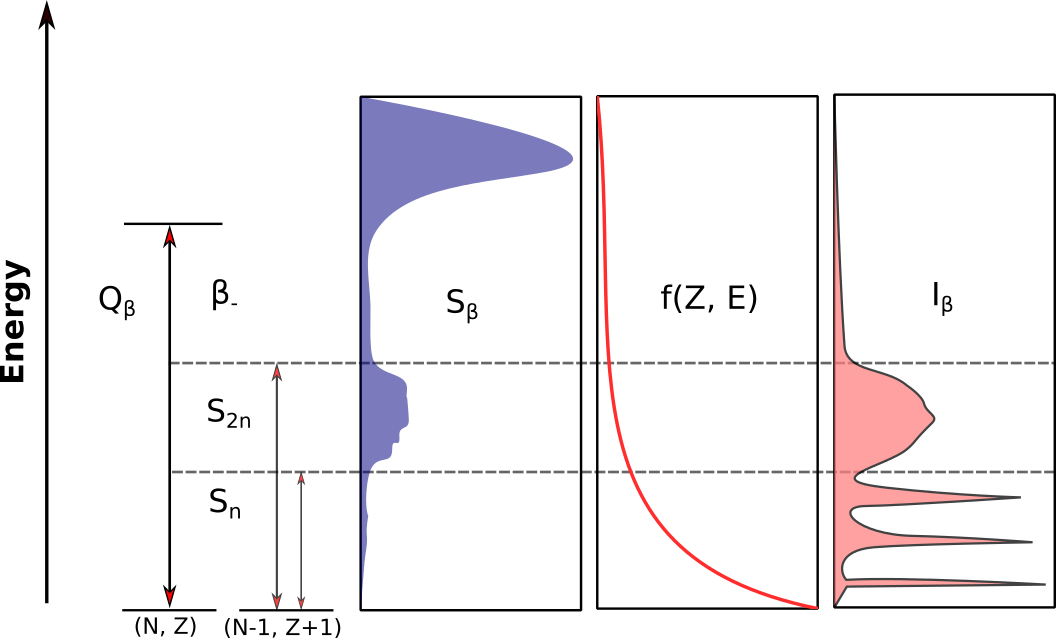
\includegraphics[width=16cm, height=10cm]{figures/strength_distribution.png}
	\caption[]{A schematic showing the decay of a $\beta$-delayed neutron precursor and the associated strength at excitation energy. The phase-space factor curtails $I_{\beta}$ at high excitation energies and augments it at lower energy.   }
	\label{fig:strength_distribution}
\end{figure}



\section{\textbf{r-process} and its role in nucleosynthesis}
The synthesis of nuclei beyond iron is attributed to the capture of neutrons by seed nuclei under extreme conditions. The processes known to play an essential part in this phenomena are r-process (rapid) and s-process (slow) \citep{burbridge}, where neutron capture reaction rates are relative to the $\beta$-decay time scales. For r-process $\tau_{n}$ $\ll$ $\tau_{\beta}$, whereas for s-process its the opposite case $\tau_{n}$ $\gg$ $\tau_{\beta}$. Considering the time scales, neutron capture path in s-process is close to the line of stability, and the nuclei involved in due course can be easily studied experimentally. r-process, on the other hand, will proceed into the very neutron-rich side far from the valley of stability. Once the neutron flux is exhausted, the unstable nuclei will decay back to the line of stability forming the stable r-process nuclei. 

\begin{figure}[h]
	\centering
	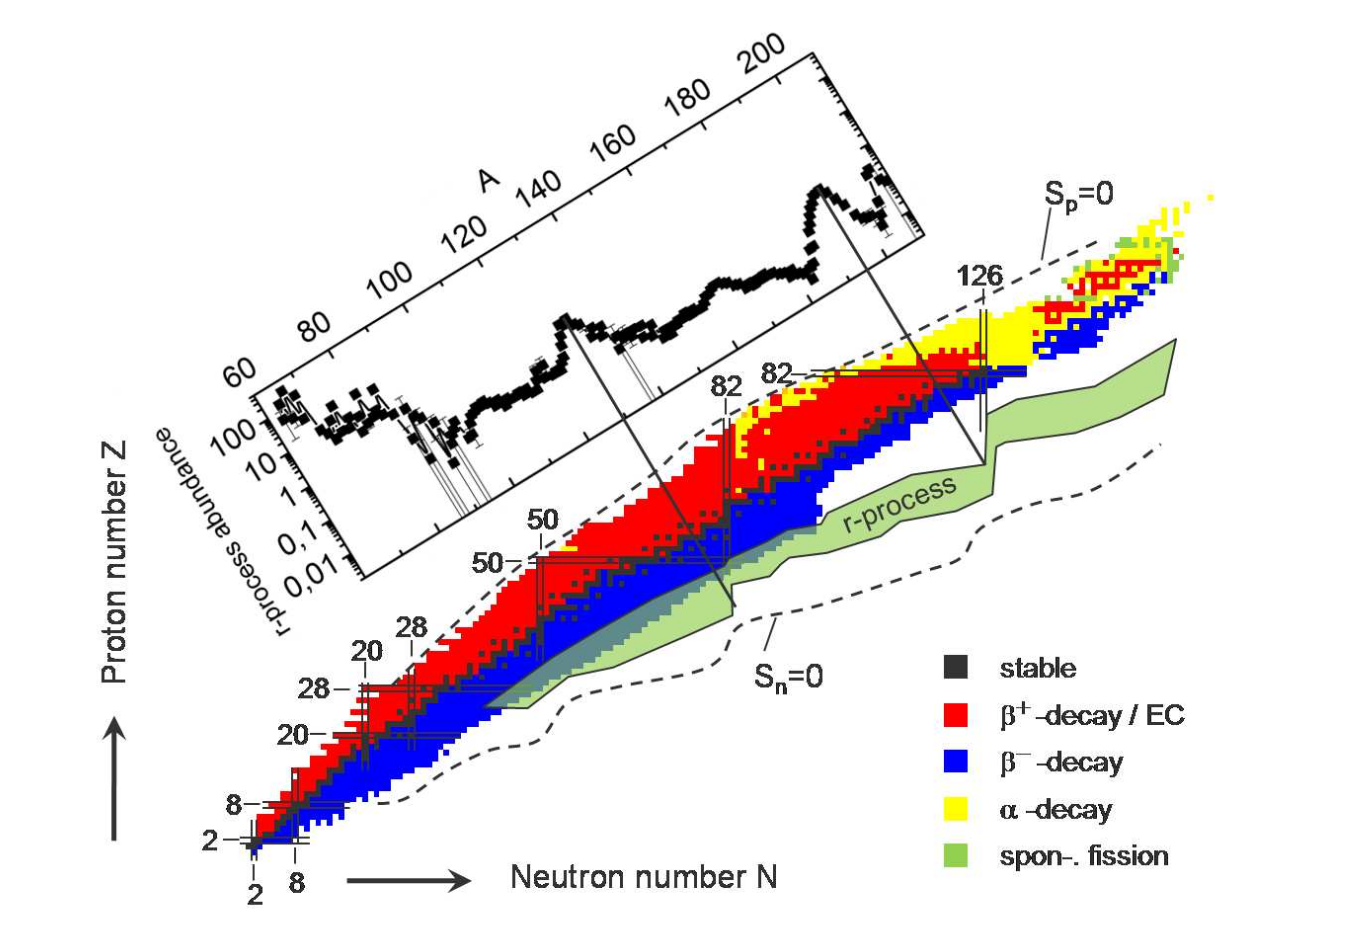
\includegraphics[width=15cm, height=10cm]{figures/r_process_path_way.png}
	\caption[Nuclei chart showing color-coded regions of stability]{Nuclei chart showing color-coded regions of stability, $\beta$-decay, $\alpha$-decay, and the r-process path. The r-process nuclei abundance pattern overlaid on the top-left demonstrates the peaks near closed nuclear-shells (Magic numbers) \citep{newmagicnumbers}.}
	\label{fig:r_process}
\end{figure}
The r-process path connects the isotopes with the maximum abundance in each isotopic chain. $\beta^{-}$-decays transfer nuclei from one isotopic chain to the next and determine the speed of the process. Abundance peaks occur due to long $\beta$-decay half-lives where the flow path comes closest to stability(closed neutron shells). The knowledge of $S_{n}$ and $\beta$-decay half-lives is helpful in determining the shape of the abundance curves.

Given the conditions conducive to r-process, experimental measurements are very challenging. The experimental bottleneck of synthesizing nuclei in the unexplored region of the chart of nuclei has been recently unblocked by a few facilities, thereby opening a whole new window to a plethora of information regarding mass and half-lives about the participating elements.

One of the significant challenges of our day is the determination of the site or sites for the r-process and therefore the identification of the origin of more than half of all the elements heavier than iron. The answer is complex and highly intermingled between the astrophysics that describes the conditions of the relevant scenarios and the physics of nuclei that operates in those scenarios. The sites of r-process have not been unambiguously identified, but a large number of neutrons required on short time scales hints at large neutron densities which are seen in explosive environments. The two leading candidates are type II (core‐collapse) supernova explosions and neutron star mergers. A recent observation of neutron star merger GW170817 \citep{gw170817} in various regions of the electromagnetic spectrum helps to narrow r-process sites. The observations suggest that the later part of the light curve produced by the post-merging supernova is backed by the radioactivity of lanthanides produced by r-process. 

\section{Nuclear structure}


The models used to define the structure of a nucleus are broadly classified into two categories, collective or independent. Collective models assume that nucleons interact strongly in the nucleus and their mean free path is small, whereas, independent models assume that the nucleons interact under the realm of Pauli principle in the nuclear matter and this leads to a larger mean free path. Now, models such as liquid drop model (collective), provides a good description of average behavior occurrence of binding energy pertaining to odd-even behavior, but it does not provide with the explanation of appearance of magic numbers of nucleons. This is mainly due to a structure of shells that cannot be obtained by the liquid drop model. Hence, there is a need to treat nucleus as a quantum system to provide with a justification for this behaviour. 

Moving on to the Fermi Gas Model, which falls under the category of independent models, is based on the notion of nucleons moving freely in the nucleus due to the Pauli principle. A nucleon in the nucleus feels the force of attraction created by all the nucleons around it. The situation can be imagined as to be similar to a balloon, inside of which nucleons can move freely, but occupy different states. The Fermi gas model, despite its simplicity explains many of the nuclear properties, it explains the lesser number of proton compared to protons as we go from from low A to high A nuclei, which is due to shallowing of proton well because of the coulomb repulsion between protons. Another explained characteristic is the high abundance of even-even nuclei compared to odd-odd nuclei. This is explained by the possibility of an isolated neutron or protons (each in their respective potential wells) in odd-odd nuclei to crossover to the well of the other via $\beta$-emission, returning to stability.


The shell model also follows the idea of nucleons moving independently of each other in the nucleus similar to the Fermi gas model. The difference here from the Fermi gas model is the introduction of a central potential, similar to the potential that acts on electrons in an atom. The central potential is the average potential created by all the nucleons in a nucleus. A nucleon is thus under the influence of a potential created by the rest of the nucleons in the nucleus. The potential should be determined in such a way to best produce the experimental results.

To give a mathematical form to the shell model, the Hamiltonian of a system consisting of A bodies can be written as

\begin{equation}
H = \sum_{i}^{A} T_{i}(r_{i}) + V(r_{1},......,r_{A})
\end{equation}
where T is the kinetic energy operator and V the potential function.
Now, if the interaction is restricted to two body the Hamiltonian assumes the mathematical form as follows:

\begin{equation}
H = \sum_{i}^{A} T_{i}(r_{i}) + \frac{1}{2}\sum_{ji}^{}V_{ij}(r_{i},r_{j}),
\end{equation}
In the shell model construct, a nucleon $\textit{i}$ feels not just the potential $\sum_{j}^{}V_{ij}$, but a central potential $U(r_{i})$, that depends only on the coordinates of nucleon $\textit{i}$. This potential can be introduced in the Hamiltonian as follows:
\begin{equation}
H = \sum_{i}^{A} T_{i}(r_{i}) + \sum_{i}^{A}U(r_{i}) + H_{res},
\end{equation}

$H_{res}$ is called the residual interaction, its part of the potential V not incorporated in the central potential U.
\begin{equation}
H_{res} = \frac{1}{2}\sum_{ji}^{}V_{ij}(r_{i},r_{j}) - \sum_{i}^{A}U(r_{i}),
\end{equation}

The $H_{res}$ term is generally anticipated to have a very small/negligible contribution to the \textit{shell model Hamiltonian}. 

The shape of the central potential should capture the features of the nucleus, i.e, the potential being maximum at the core and gradually waning closer to the radius. A potential called "Woods-Saxon" form is generally used to capture the features mentioned. Its mathematically defined as:
\begin{equation}
U(r) = \frac{U_{0}}{1+exp(\frac{r-R}{a})} 
\end{equation}

where $U_{0}$, R, and a represent as potential well depth, radius of the nucleus, and surface thickness, respectively.

The Schrodinger equation with the Hamiltonian H can be solved numerically providing wave functions of protons and neutrons characterized by shell (n), orbital (l), and total angular momentum (j) quantum numbers.


\begin{figure}[h!]
	\centering
	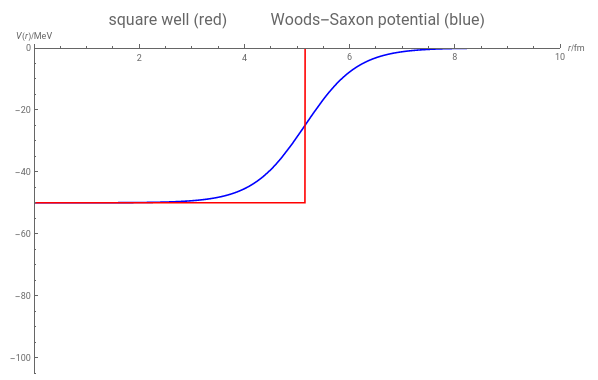
\includegraphics[width=12cm,height=10cm]{figures/Wood_sxaon.png}
	\caption[Wood-Saxon and square well potential for a nucleus with A = 70, $U_{0}$=50 MeV, and a = 0.5 fm.]{Wood-Saxon and square well potential for a nucleus with A = 70, $U_{0}$=50 MeV, and a = 0.5 fm. The plots demonstrates the shape of the Wood-saxon potential (blue) when compared to a square well potential (red). }
	\label{fig:woods_saxon}
\end{figure}
A considerable improved in matching the results was provided upon the addition of a spin-orbit interaction term to the Hamiltonian. The spin-orbit interaction term removes the degeneracy in the total angular momentum state \textit{j}. 


\begin{figure}[h!]
	\centering
	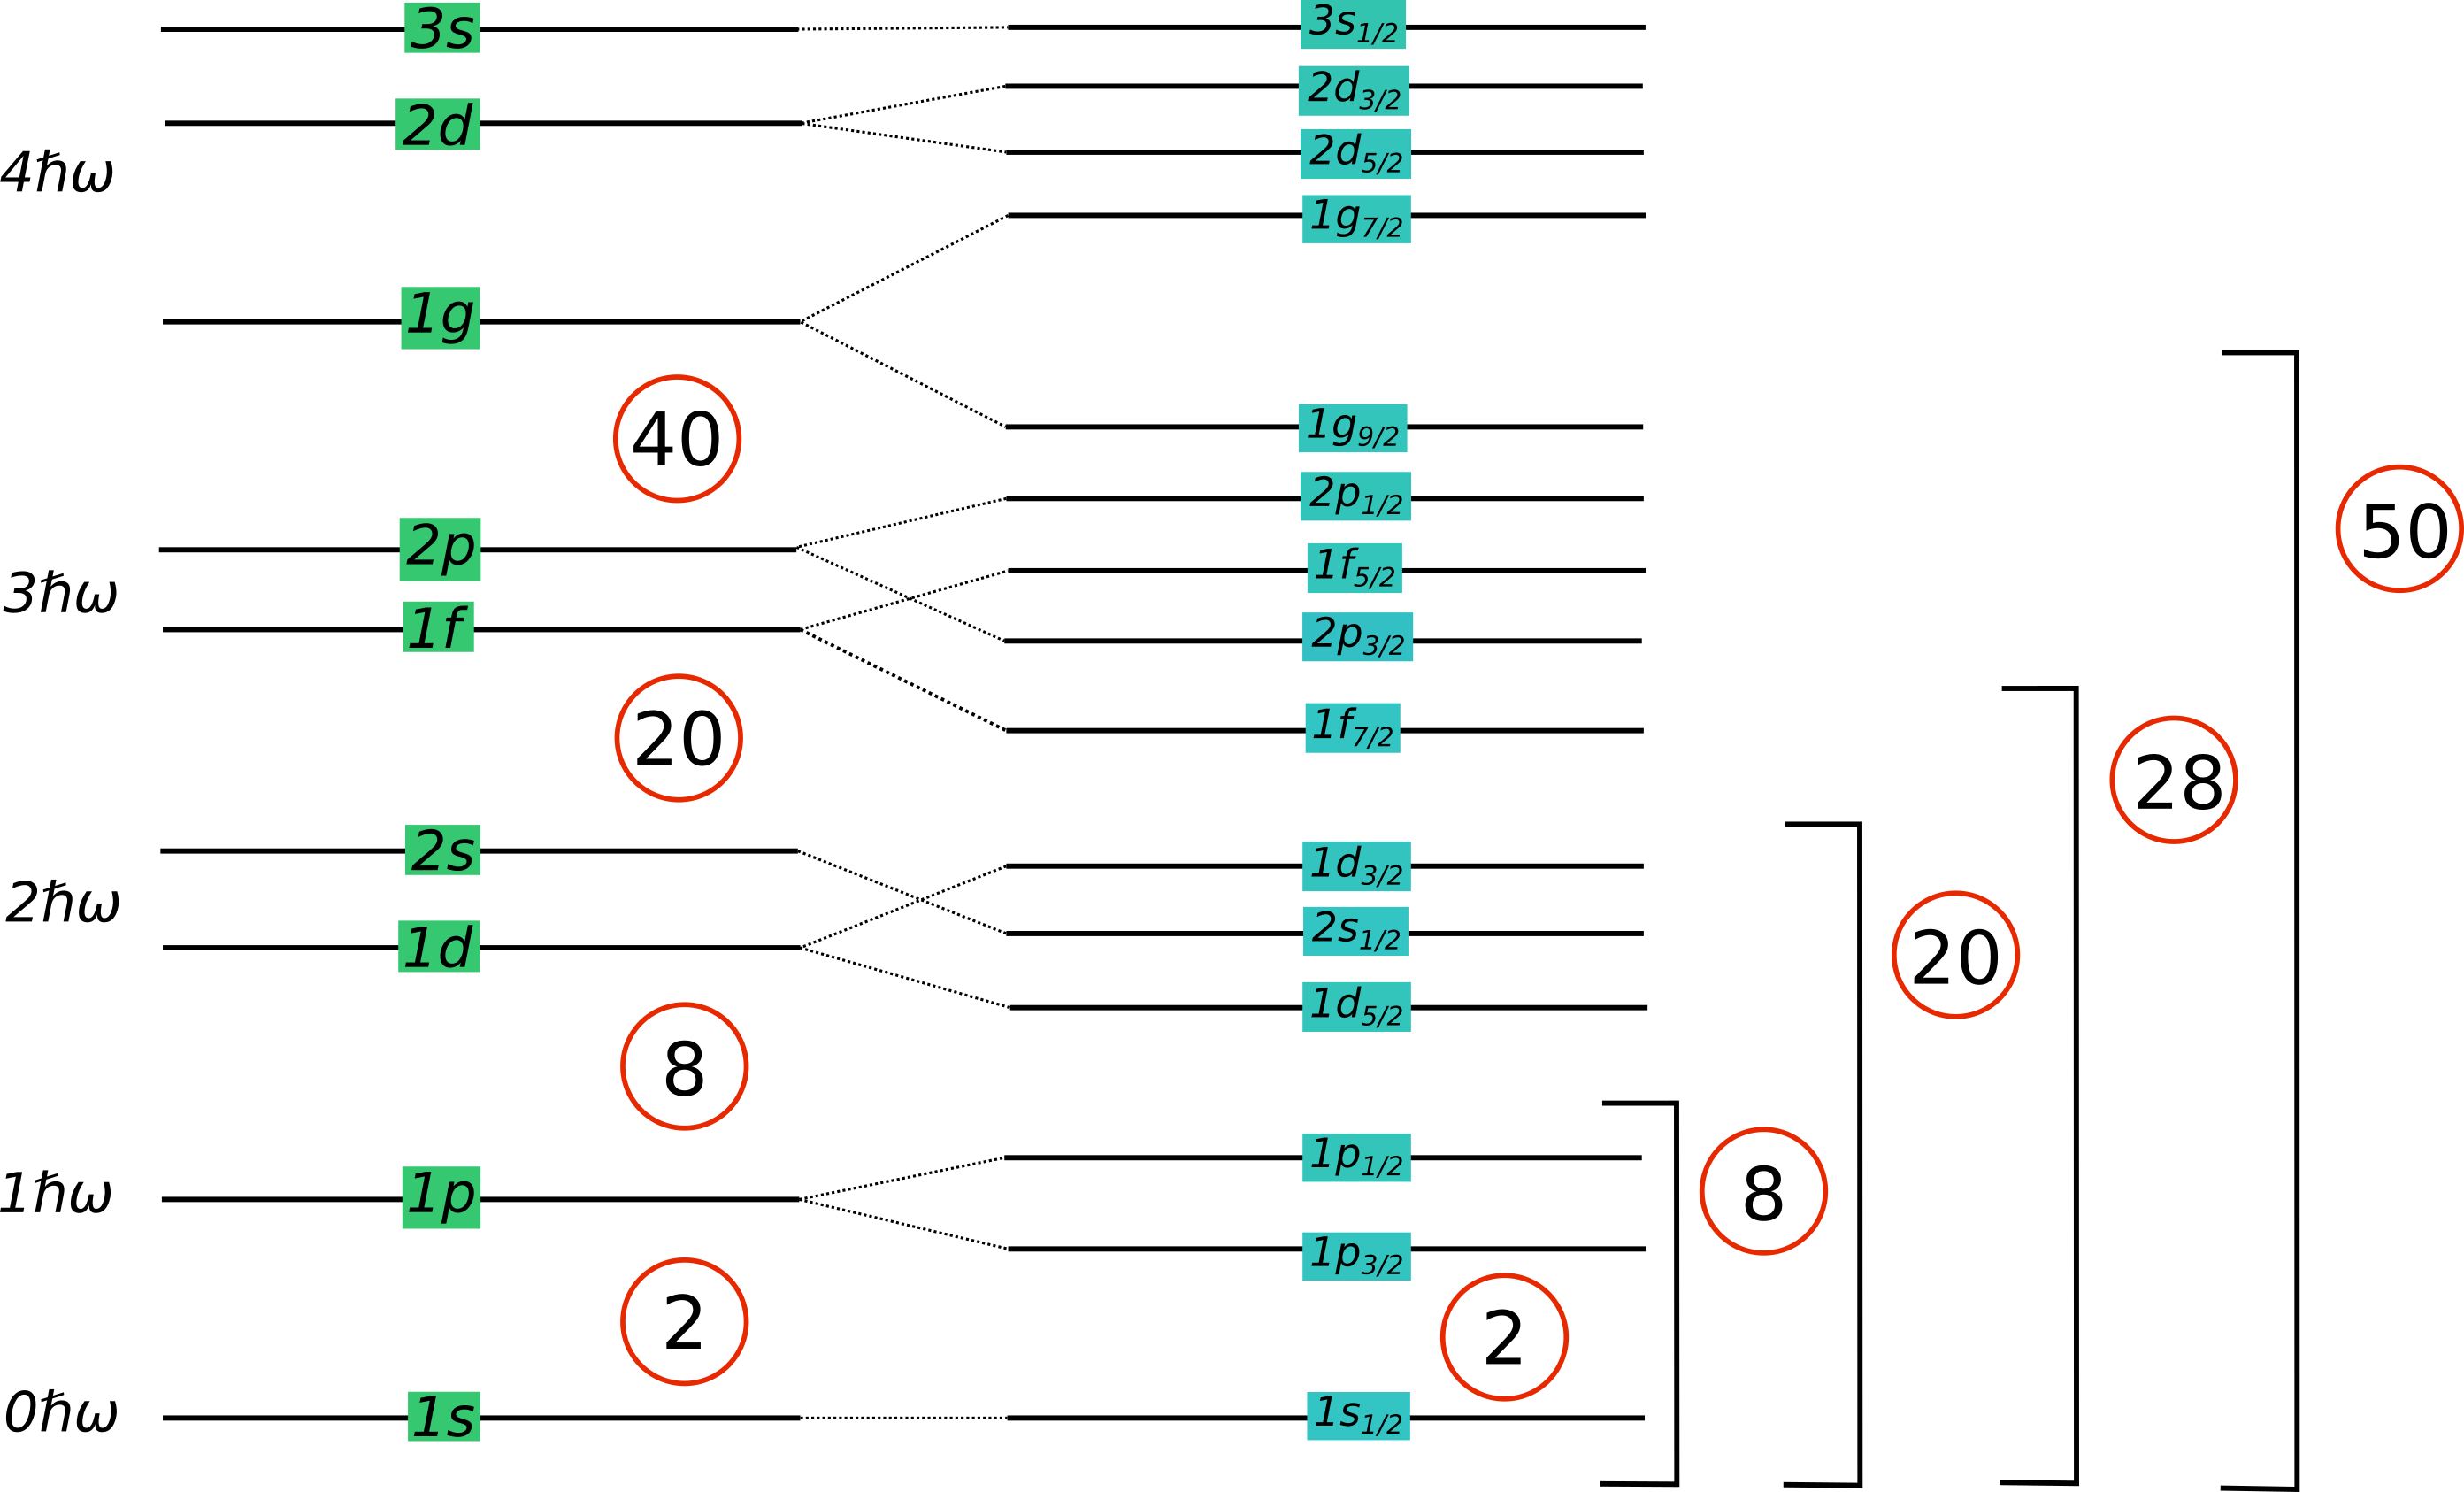
\includegraphics[width=17cm,height=10.5cm]{figures/shell_model.png}
	\caption[Level scheme of the shell model showing the breaking of degeneracy]{Level scheme of the shell model showing the breaking of degeneracy in the energy levels due to the spin-orbit interaction term. There is an emergence of some new magic numbers in the shell closing such as 28 and 50. The level scheme is not concrete and is expected to change as per the nuclear potential chosen.}
	\label{fig:shell_structure}
\end{figure}
After the discussion on the structure of an atomic nucleus using Shell model, we can rehash that an atomic nucleus is a quantum many-body system whose constituent nucleons (protons and neutrons) are subject to complex nucleon-nucleon interactions that include spin- and isospin-dependent components. For stable nuclei, the seemingly emerging patterns in some observables, such as the shell closure for neutrons or protons in nuclei: N, Z = 8, 20, 28, 50, 82, 126 can be explained with great success using shell-model calculations. 
\begin{figure}[h!]
	\centering
	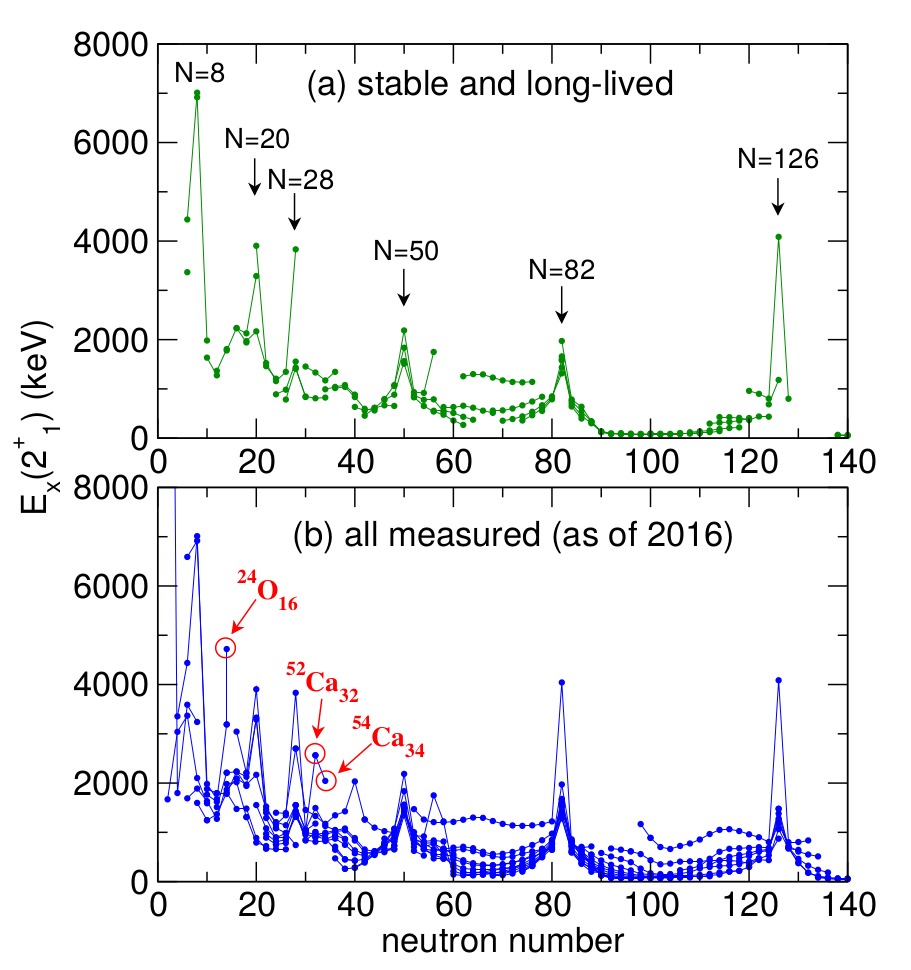
\includegraphics[width=14cm,height=14cm]{figures/be2_n_50.png}
	\caption[Systematics of the $2\textsuperscript{+}$ excitation energy  ]{Systematics of the $2\textsuperscript{+}$ excitation energy for a) stable istopes and b) all nuclei measurements upto 2016. pritychenko et al., 2016 }
	\label{fig:2_plus_excitation}
\end{figure}

The testing of the shell model has been predominantly for stable nuclei and their neighbouring isotopes. The dynamics of interaction of nucleons in a nuclei starts to take a different turn with the addition of more neutrons/protons, mainly due to N/Z ratio deviating heavily from one. The picture of nuclear structure is quite different for nuclei far-off stability, these nuclei are also termed as "exotic." These exotic nuclei imply atomic nuclei with an unbalanced N/Z ratio as compared to stable ones, thus losing binding energy due to a large difference in Z and N (Bethe and Bacher, 1936; von Weizsäcker, 1935). Relatively smaller binding energies mean that $\beta$-decay channels open up, proceeding towards more N/Z balanced systems and resulting infinite (often short, sub-second, milliseconds) lifetimes. The asymmetry in N/Z ratio along with an interplay of nuclear forces can lead to emergence of new shell closures and shape deformations. The phenomena of change in the orientation of nuclear orbitals with the addition of more neutron/protons in stable isotopes is called "Shell Evolution." 

As an example of the shell evolution, systematics of the first $2\textsuperscript{+}$ levels is shown in the Figure \ref{fig:2_plus_excitation}. Part (a) of the figure shows appearance of magic numbers as predicted by the shell model having higher first $2\textsuperscript{+}$ excitation energy. Part (b) of the figure shows the data for nuclei measured until 2016, highlighting a relatively high $2\textsuperscript{+}$ excitation energy not predicted by shell-model, and displays the effects of shell evolution in structural properties.

The questions surrounding patterns in structure beyond stability can be answered by exploring various types of nuclear forces. The effects of nuclear forces affecting the shell structure can be studies in terms of their monopole component ot play. The monopole matrix element of an interaction, $\hat V$ is defined as 

\begin{equation}
v\textsubscript{m;j, j'} = \frac{\sum_{k, k'}^{}\langle jkj'k'|\hat V|jkj'k'\rangle}{\sum_{k, k'}^{}1},
\end{equation}
where $\textit{j}$ and $\textit{j'}$  denote the single-article angular momentum quantum numbers with $\textit{k}$ and $\textit{k'}$ denoting their respective magnetic substate, and quantity $\langle ...|\hat V|...\rangle$ is anti-symmetric in nature as per Pauli exclusion principle. Equation 1.19 shows the averaging over all possible orientations of two interacting particles in orbitals $\textit{j}$ and $\textit{j'}$. The monopole component of $\hat V$ is written, for $\textit{j}$ $\not=$ $\textit{j'}$, as 

\begin{equation}
\hat v_{m; j, j'} = v_{m;j,j'}\hat n_{j} \hat n_{j'},
\end{equation}


where the $\hat n_{j} (\hat n_{j'})$ is the number operator of the orbits $\textit{j (j')}$. The monopole component of the operator $\hat V$, as shown above is the average of all effects of $\hat V$, and it depends only on the occupation number of the orbits involved. Using neutron-proton scheme monopole interaction can be used with the convention: $n_{j}$ and $n_{j'}$ as the occupation number for protons and for neutrons in the orbits, respectively.


The shift in the single-particle energy (SPE) of proton orbits ($\textit{j}$) with the addition of neutrons in orbits ($\textit{j'}$) due to the monopole interaction can be written as 

\begin{equation}
\Delta \epsilon_{j} = v_{m;j,j'}n_{j'}.
\end{equation}


Due to linerarity of the monopole interaction, the effect of the monopole interaction can be magnified to a large degree with the increase in occupation of nucleons in valence orbit $\textit{j'}$, when we move away from the stability towards the neutron-rich side. As an example, Figure \ref{fig:monopole_interaction} depicts the monopole interactions that can take place as we keep filling neutrons in the $1g\textsubscript{9/2}$ (N$>$40) state, lying above the N=40 core. Single-particle proton states for Z $>$ 28 can be filled in $2p\textsubscript{3/2}$, $1f\textsubscript{5/2}$, and $2\textsubscript{1/2}$. 

\begin{figure}[h!]
	\centering
	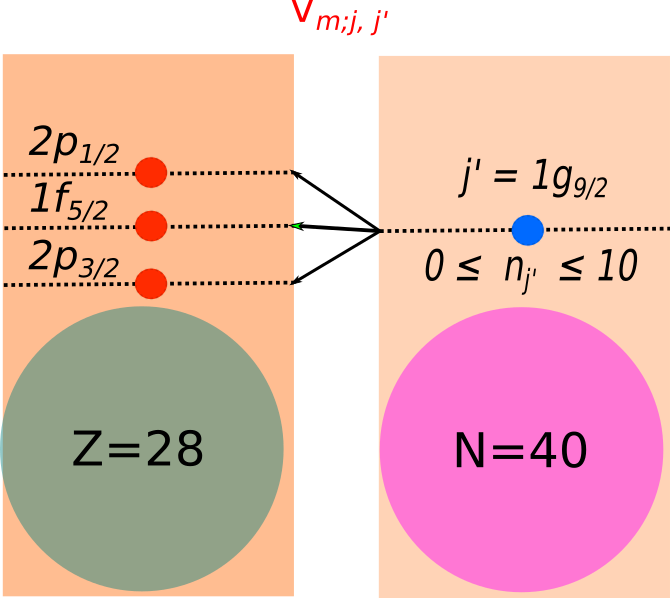
\includegraphics[width=10cm,height=9cm]{figures/monopole_text.png}
	\caption[A graphical demonstration of the monopole interaction between the neutron single-particle state ]{A graphical demonstration of the monopole interaction between the neutron single-particle state $1g\textsubscript{9/2}$ and the proton single-particle states $2p\textsubscript{3/2}$, $1f\textsubscript{5/2}$, and $2\textsubscript{1/2}$. The shift in the energy of the state $1f\textsubscript{5/2}$ is larger compares to the shift for $2p\textsubscript{3/2}$ and $2p\textsubscript{1/2}$ due to a large radial overlap ($\Delta l = 1$) between the $\textit{f}$ and $\textit{g}$ shells. }
	\label{fig:monopole_interaction}
\end{figure}
The residual interaction can also have contributions from the spin-isospin interaction {reference from otsuka paper 2013}, which explain the appearance of magic numbers at Z=14 and N = 16. The tensor force {reference from otsuka paper 2013} due to pion exchange is another contribution to the residual interaction that has been explored for some nuclei.

\subsection{Shell evolution of Cu isotopes}


The sections above lay the basic foundation of structure of a nucleus and its evolution upon stuffing it with more and more neutrons due to the the monopole part of the nuclear forces. Here we discuss the shell evolution of $\textsubscript{29}$Cu isotopes. Copper isotopes display a great deal of shell-migration due to monople interaction and also display display competition between single-partcile and collective modes at low excitation energies [shell quenching in \textsuperscript{78}Ni [5-7]]. The idea of migration of states was seeded with the observation of lowering of $5/2^{-}$ in \textsuperscript{73,71}Cu [shell quenching in \textsuperscript{78}Ni 8]. This lead to a belief that $5/2^{-}$ may eventually become ground-state in \textsuperscript{75}Cu. $5/2^{-}$ was later confirmed as the ground state in \textsuperscript{75}Cu via magnetic moment measurements in the copper chain [shell quenching in \textsuperscript{78}Ni [7]]. The inversion was also predicted to be prevalent in  \textsuperscript{77,79}Cu. Figure \ref{fig:5_2_sytematics} shows the trend in the energy of the $5/2^{-}$ and $3/2^{-}$ states with the increase in neutron number. The observed trends in the energy of the low-lying states also point to the questioning of the Z=28 shell gap. There have been suggestion of the thinning in the Z=28 shell-gap. Studies mentioned in [persistance of shell-gap [23,24]] suggest a weakening of the Z=28 shell gap but the idea could not be substantiated with experimental measurements. However, half-life measurements hint at the survival of \textsuperscript{78}Ni doubly-magic (Z=28; N=50) characteristics with first excited state at $\sim$ 2 MeV. $\gamma$-ray measurements of the \textsuperscript{80}Zn(\textit{p,2p})\textsuperscript{79}Cu at RIBF ascertained the persistence of Z=28 shell-gap [persistance of shell-gap]. The findings of the experiment suggest at considering $\textsuperscript{29}$Cu consisting of a $\textsuperscript{78}$Ni with a valence proton, as depicted in Figure \ref{fig:Cu79_cartoon}. \textsuperscript{78}Ni was eventually identified to be doubly-magic with its $2^{+}$ state lying at 2.6 MeV [nature article] using in-beam $\gamma$-ray spectroscopy of \textsuperscript{80}Zn(\textit{p,3p})\textsuperscript{78}Ni reaction. Now to have a rather much closer look at the structure of $\textsuperscript{29}$Cu, $\beta$-decay strength distributions will be a useful tool to identify the strongest connecting states and the occupation of protons in excited states above $1f_{5/2}$. Read miguel's paper and draw ideas 


\begin{figure}[h]
	\centering
	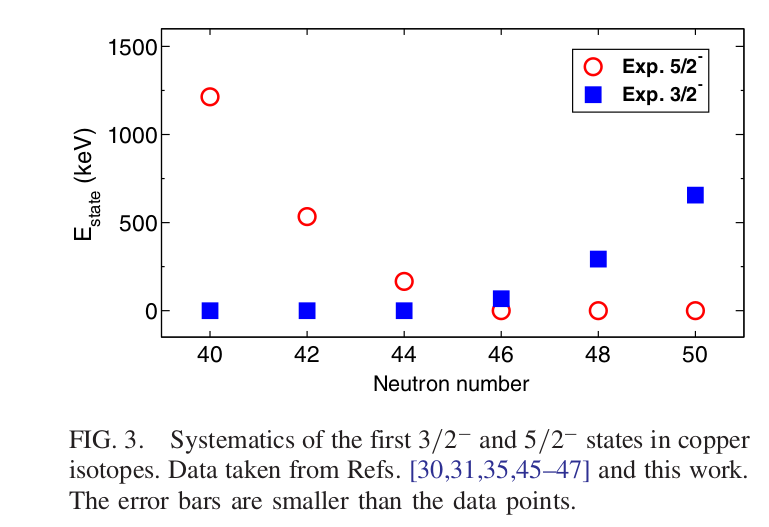
\includegraphics[width=14cm,height=10cm]{figures/Cu_5_2_sytematics.png}
	\caption[Systematics of the  $5/2^{-}$ and  $3/2^{-}$ for odd-even Cu isotopes. ]{Systematics of the  $5/2^{-}$ and  $3/2^{-}$ for odd-even Cu isotopes. create your own picture using the data. }
	\label{fig:5_2_sytematics}
\end{figure}


\begin{figure}[h]
	\centering
	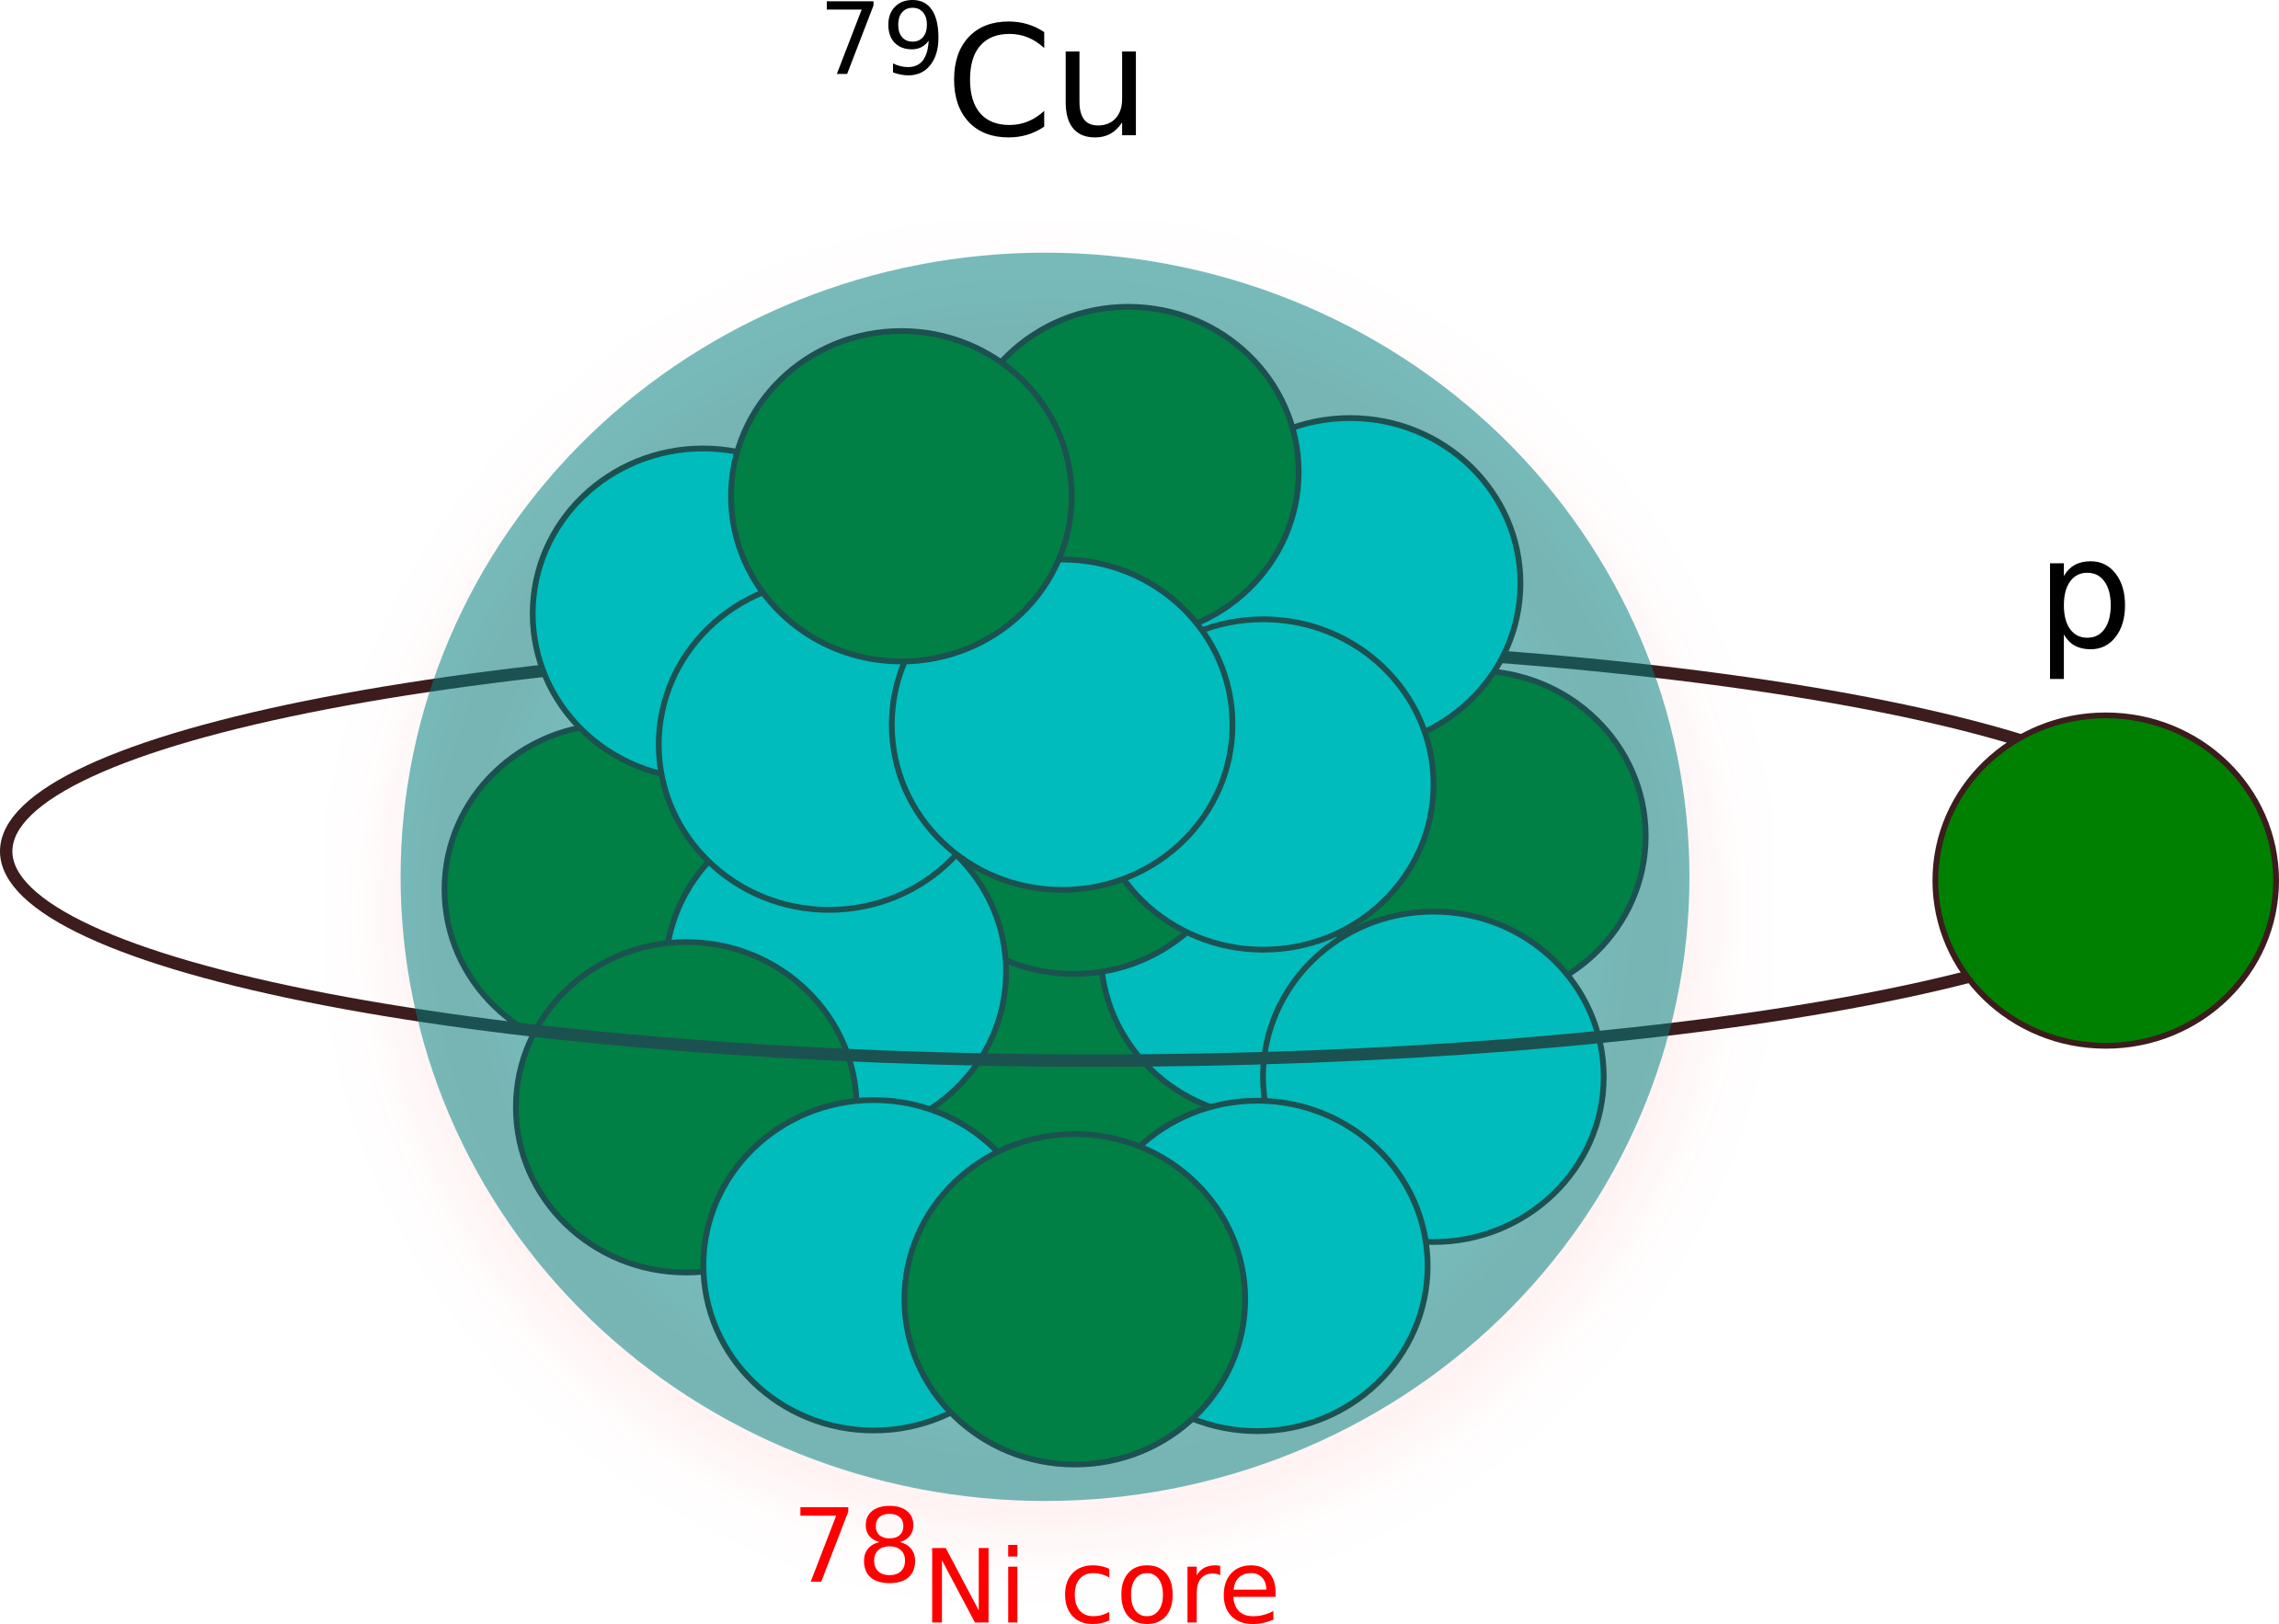
\includegraphics[width=10.5cm,height=8cm]{figures/Cu79_cartoon.png}
	\caption[$\textsuperscript{29}Cu$ depicted as having a $\textsuperscript{78}Ni$ core]{$\textsuperscript{29}Cu$ depicted as having a $\textsuperscript{78}Ni$ core and a valence proton orbiting in the $1f_{5/2}$ state as a ground state. }
	\label{fig:Cu79_cartoon}
\end{figure}




gather Cu isotopes information and show shell-evolution 

shell gap persistence 

whats beyond N>50, n>52

define the research gaps and fill in the information and mostly what my works provides and how it pushes the envelope.




    \chapter{Implantation detector development} \label{ch:yso_detector}

\section{Particle Detection using Scintillators}
Scintillators are one of the oldest materials to be used for particle detection and identification. The idea of using the scintillators dates back to the early 1900s \citep{rutherford} when Ernest Rutherford discovered $\alpha$-particles with the aid of scintillator Zinc sulfide (ZnS). In the following years huge strides were made in the development and implementation of these materials in various sectors of research and industry.\\

The materials falling under the category of scintillators are broadly categorized as organic and inorganic scintillators. The scintillation mechanism depends on the structure of the crystal lattice. Here the focus is on inorganic scintillators (halides, oxides, chalcogenides, and glasses). The basic concept behind the particle or incident gamma-ray detection using a scintillator is the conversion of the energy lost in the material into light, which is emitted in a specific wavelength band of the Electromagnetic spectrum. 
The ionizing radiation upon interaction leaves the system in a state of non-equilibrium, and the tendency to reach a state of equilibrium is lead by a multitude of elementary processes, such as the creation of primary electronic excitation which will produce an avalanche of secondary particles including electrons, holes, photons, and plasmons. These electronic excitations produce numerous thermalized electron-hole(e-h) pairs and low energy excitons which ultimately transform into light photons, i.e., scintillation. The following steps can broadly describe the scintillation process:
\begin{enumerate}
	\item Absorption of the ionizing radiation and creation of primary electrons and holes.
	\item Relaxation of the primary electrons and holes, thereby production of many secondary electrons, holes, protons, plasmons, and other electronic excitations.
	\item Thermalization of the low-energy secondary electrons (holes) resulting in a number if e-h pairs with energy roughly equal to the band-gap energy $E_{g}$.
	\item Energy transfer from e-h pairs to the luminescence centers and their excitation.
	\item Emission from the luminescence centers.
\end{enumerate}
\begin{figure}[h!]
	\centering
	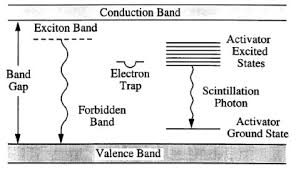
\includegraphics[width=10cm,height=8cm]{figures/inorganic_scintillators_mechanism.jpeg}
	\caption[A schematic diagram explaining the scintillation]{A schematic diagram explaining the scintillation mechanism in inorganic scintillators. }
	\label{fig:scintillation_mechanism}
\end{figure}



\subsection{Charged Particles}
A charged particle in its passage through the volume of the material exhausts its kinetic energy in excitation and ionization of atoms. These kinds of energy losses are labeled as ionization losses. What we observe then is a statistical average of the two processes occurring as the particle slows down. The stopping power S (dE/dx) of the matter is determined concerning the energy lost (dE) by the particle in infinitesimal distance (dx): the higher the stopping power, the shorter the range into the material the particle can penetrate. The quantity S is also referred to as \textit{specific energy loss}. The average ionization losses of a charged particle are given by the well known Bethe-Bloch formula \citep{bethebloch}.

\begin{equation}
-\frac{dE_{ion}}{dx}=\frac{4\pi N_{A} Z^{2} e^{4}}{m_{e} V^{2}} \frac{z}{a} \Bigg[ ln\Bigg(   \frac{2mV^{2}}{\overline{I} (1-\beta^{2})}    \Bigg) -\beta^{2}\Bigg],
\end{equation}


Where z, m, and V are the charge, mass, and velocity of the particle, respectively; \textit{x} (cm\textsuperscript{2}/g) is the path of the particle into the matter; Z and A are the atomic and mass number of the matter, respectively; $N_{A}$ is the Avogadro number, and $\overline{I}$ is usually obtained empirically, but some estimates are made using the relation $\overline{I}$ = 13.5 Z (ev).
\newline
Following above equation, it can be inferred that ionization power of heavy charged particle (proton, $\alpha$ particle, multiply ionized atoms, etc.) is $z^{2}$ times greater than the ionization power of an electron of the same velocity. Low-energy electrons, protons, $\alpha$ particles, and heavy ions are weakly-penetrating particles requiring small scintillator thickness for stopping. The light output of the scintillator depends not only on the energy losses but also on the density of ionization. In spite of ionization losses increasing with increase the charge  and mass of the particle, there is a decline in the light output of the scintillator.

The light produced in the scintillating material by highly ionizing particles (heavy ions) is lower than that produced by electrons of the same energy. Therefore, the signal generated by the ions will be seen at lower voltages than their real values for a scintillator calibrated with electrons or $\gamma$-rays, due to the presence of light-quenching for heavy ions. A knowledge of these transformation factors is very important when it comes to detecting and interpreting heavy ions. 
Light yield dL is proportional to the energy-loss (dE) by the particle in the scintillator
\begin{equation}
dL = SdE
\end{equation}

where S is the absolute scintillation factor. In differential form, the above equation is written:

\begin{equation}
\frac{dL}{dx}= S\frac{dE}{dx}
\end{equation}

The suppression for the light yield for the heavy ions is suggested by Birks Relation

\begin{equation}
\frac{dL}{dx}= S\frac{\frac{dE}{dx}}{1+kB\frac{dE}{dr}}
\end{equation}

where B$\frac{dE}{dx}$ denotes the density of excitation centers along the track, k is the quenching factor; kB as a product is known as Birks Factor. The quenching factor for ions is the ratio of the light yield of ions relative to that of electrons at the same energy.

\begin{equation}
Q_{i}(E)=\frac{L_{i}(E)}{L_{e}(E)}
\end{equation}


\*Explain Quenching from physics point of view*\ Look in the birks book 


\subsection{Neutrons}
Neutrons interact with a solid mainly through strong interplay with the nuclei. The interaction of neutrons with the matter is mainly restricted to scattering and absorption. Elastic scattering cross-section of neutrons at low energy is given as:
\begin{equation}
\sigma_{n}=4\pi(1.4 \cdot 10^{-13} A^{1/3})^{2}
\end{equation}
Usually, crystals based on B-, Li-, and Cd are used as scintillators for detecting low energy neutrons because of the large cross-section of the elements for neutrons. With increasing energy of neutron, inelastic scattering starts to dominates.

\section{YSO (Yttrium Ortho Silicate) based Implant Detector}

Implantation detectors are employed at fragmentation beam facilities mainly to detect the tagged isotopic beam impinged on it. The impinged ions, by eventually coming to rest in the scintillator, undergo radioactive decay emitting low energy beta particles, $\gamma$-rays, alpha particles, and neutrons. Thus, a proper mechanism is needed to identify the impinged ions and correlate them to the corresponding beta event. The correlations are crucial for determining the decay half-lives, and developing decay cascade of the precursor nuclei into subsequent daughter nuclei. The correlations are drawn on a position-to-position basis of the impinged ions and the beta particles. The detector is also needed to properly tag the gamma, neutron, or alpha events for exploring the full decay perspectives of nuclei: it is helpful in calculating the branching ratios, half-lives, and energy for various decay chains- the energy of particles to be detected range from a few keV to GeV. At present, most facilities around the world, are using detectors which are silicon-based, such as AIDA \citep{AIDA}, and WAS3ABi \citep{wasabi} at RIBF, RIKEN. These detectors work well overall but fail to posses good timing resolution needed for measurements bases on Time of Flight (ToF). Further, YSO has higher stopping power than Si, requiring lesser material thickness for stopping energetic ions and also provides high light yield.
In the following section details about the construction and performance of the detector are presented.




/*Put the Rationale behind the selection of the material YSO

Discuss about its characteristics in terms of the timing and the fact that it can be segmented,
put the characteristics table here in the section.*/


YSO ($Y_{2}SiO_{5}$:Ce) scintillation crystal ($\rho$=4.44 \textit{g/$cm^{3}$}, effective Z=39) offers a good combination of properties characterizing an implantion detector. YSO emission spectrum peaks at 420 nm (refractive index = 1.8) and couples well with PSPMT under the stimulation of high energy. It also has the advantage of high light yield, good timing-resolution, short decay time, non-deliquescence, and all-around stable physical and chemical properties \citep{ysospecs}.

Using YSO, a new segmented scintillator-based detector was developed at the University of Tennessee, Knoxville. The detector unit consists of a segmented (2inch x 2inch) YSO crystal with each segment having a dimension of 1 mm $\times$ 1 mm. Each segment, as well as the face and the sides, is isolated by ESR (3M) reflector material. The crystal has a thickness of 5mm and is coupled with a flat panel multi-anode position-sensitive photo-multiplier (PSPMT) tube by Hamamatsu, H12700. There is a 2-mm thick quartz light diffuser between the YSO crystal and the PSPMT to achieve sub-anode position resolution by spreading the light from one pixel onto several anodes of the PSMT. The crystal is coupled with PSPMT using organic adhesive material, sylgard, to provide mechanical rigidity to the final detector. This design was used for BRIKEN Fall 2017 campaign.

The signals from the PSPMT are read out using a resistor network board provided by Vertilon. Signals from the detector are decoded into a position array by calculating the \textit{centroid} of the signal voltage, using what is known as \textit{Anger Logic}, also named after Hal Anger \citep{angerlogic}, who implemented it to get the positions of the nuclear events in $\gamma$-ray detectors. The idea behind Anger Logic is conceptualized as follows: if the voltage signal of a photomultiplier is made proportional to its position, the \textquotedblleft  centroid\textquotedblright of the voltages produced by a particle will determine where the particle originated-the goal of this logic. Anger Logic is needed to enhance spatial resolution; large thicknesses of scintillator material are required to improve the photon cross-section and the measurement of the photon energy, which is essential for suppression of the contribution from Compton-scattered photons. Furthermore, the segmentation of the scintillator supplements the position resolution of the particle hit-pattern. 

\subsection{YSO Detector Development for ToF based Delayed Neutron Spectroscopy}
A YSO implant detector with revised design and specifications was developed for performing ToF-based delayed neutron emission spectroscopy using VANDLE \citep{VANDLE}. The detector acts as a fast $\beta$-trigger along with recording implanted ion positions.

\subsubsection{Detector design and construction}
The detector consists of a 7.5 cm $\times$ 7.5 cm segmented array of YSO crystal with 2 mm pitch, coupled with a PSPMT by Hamamatsu, H12700B-03 (48.5 mm $\times$ 48.5 mm effective area), via a tapered and pixelated acrylic light guide. The light guide is used to focus the light produced through scintillation in YSO onto the face of the PSPMT. A one-to-one correspondence between the pixels of the crystal and the light guide is ensured by UV curing the two with each other. The combined crystal and light guide system is coupled with the PSPMT using sylgard, providing optical coupling and mechanical stability. 
\begin{figure}[h!]
	\centering
	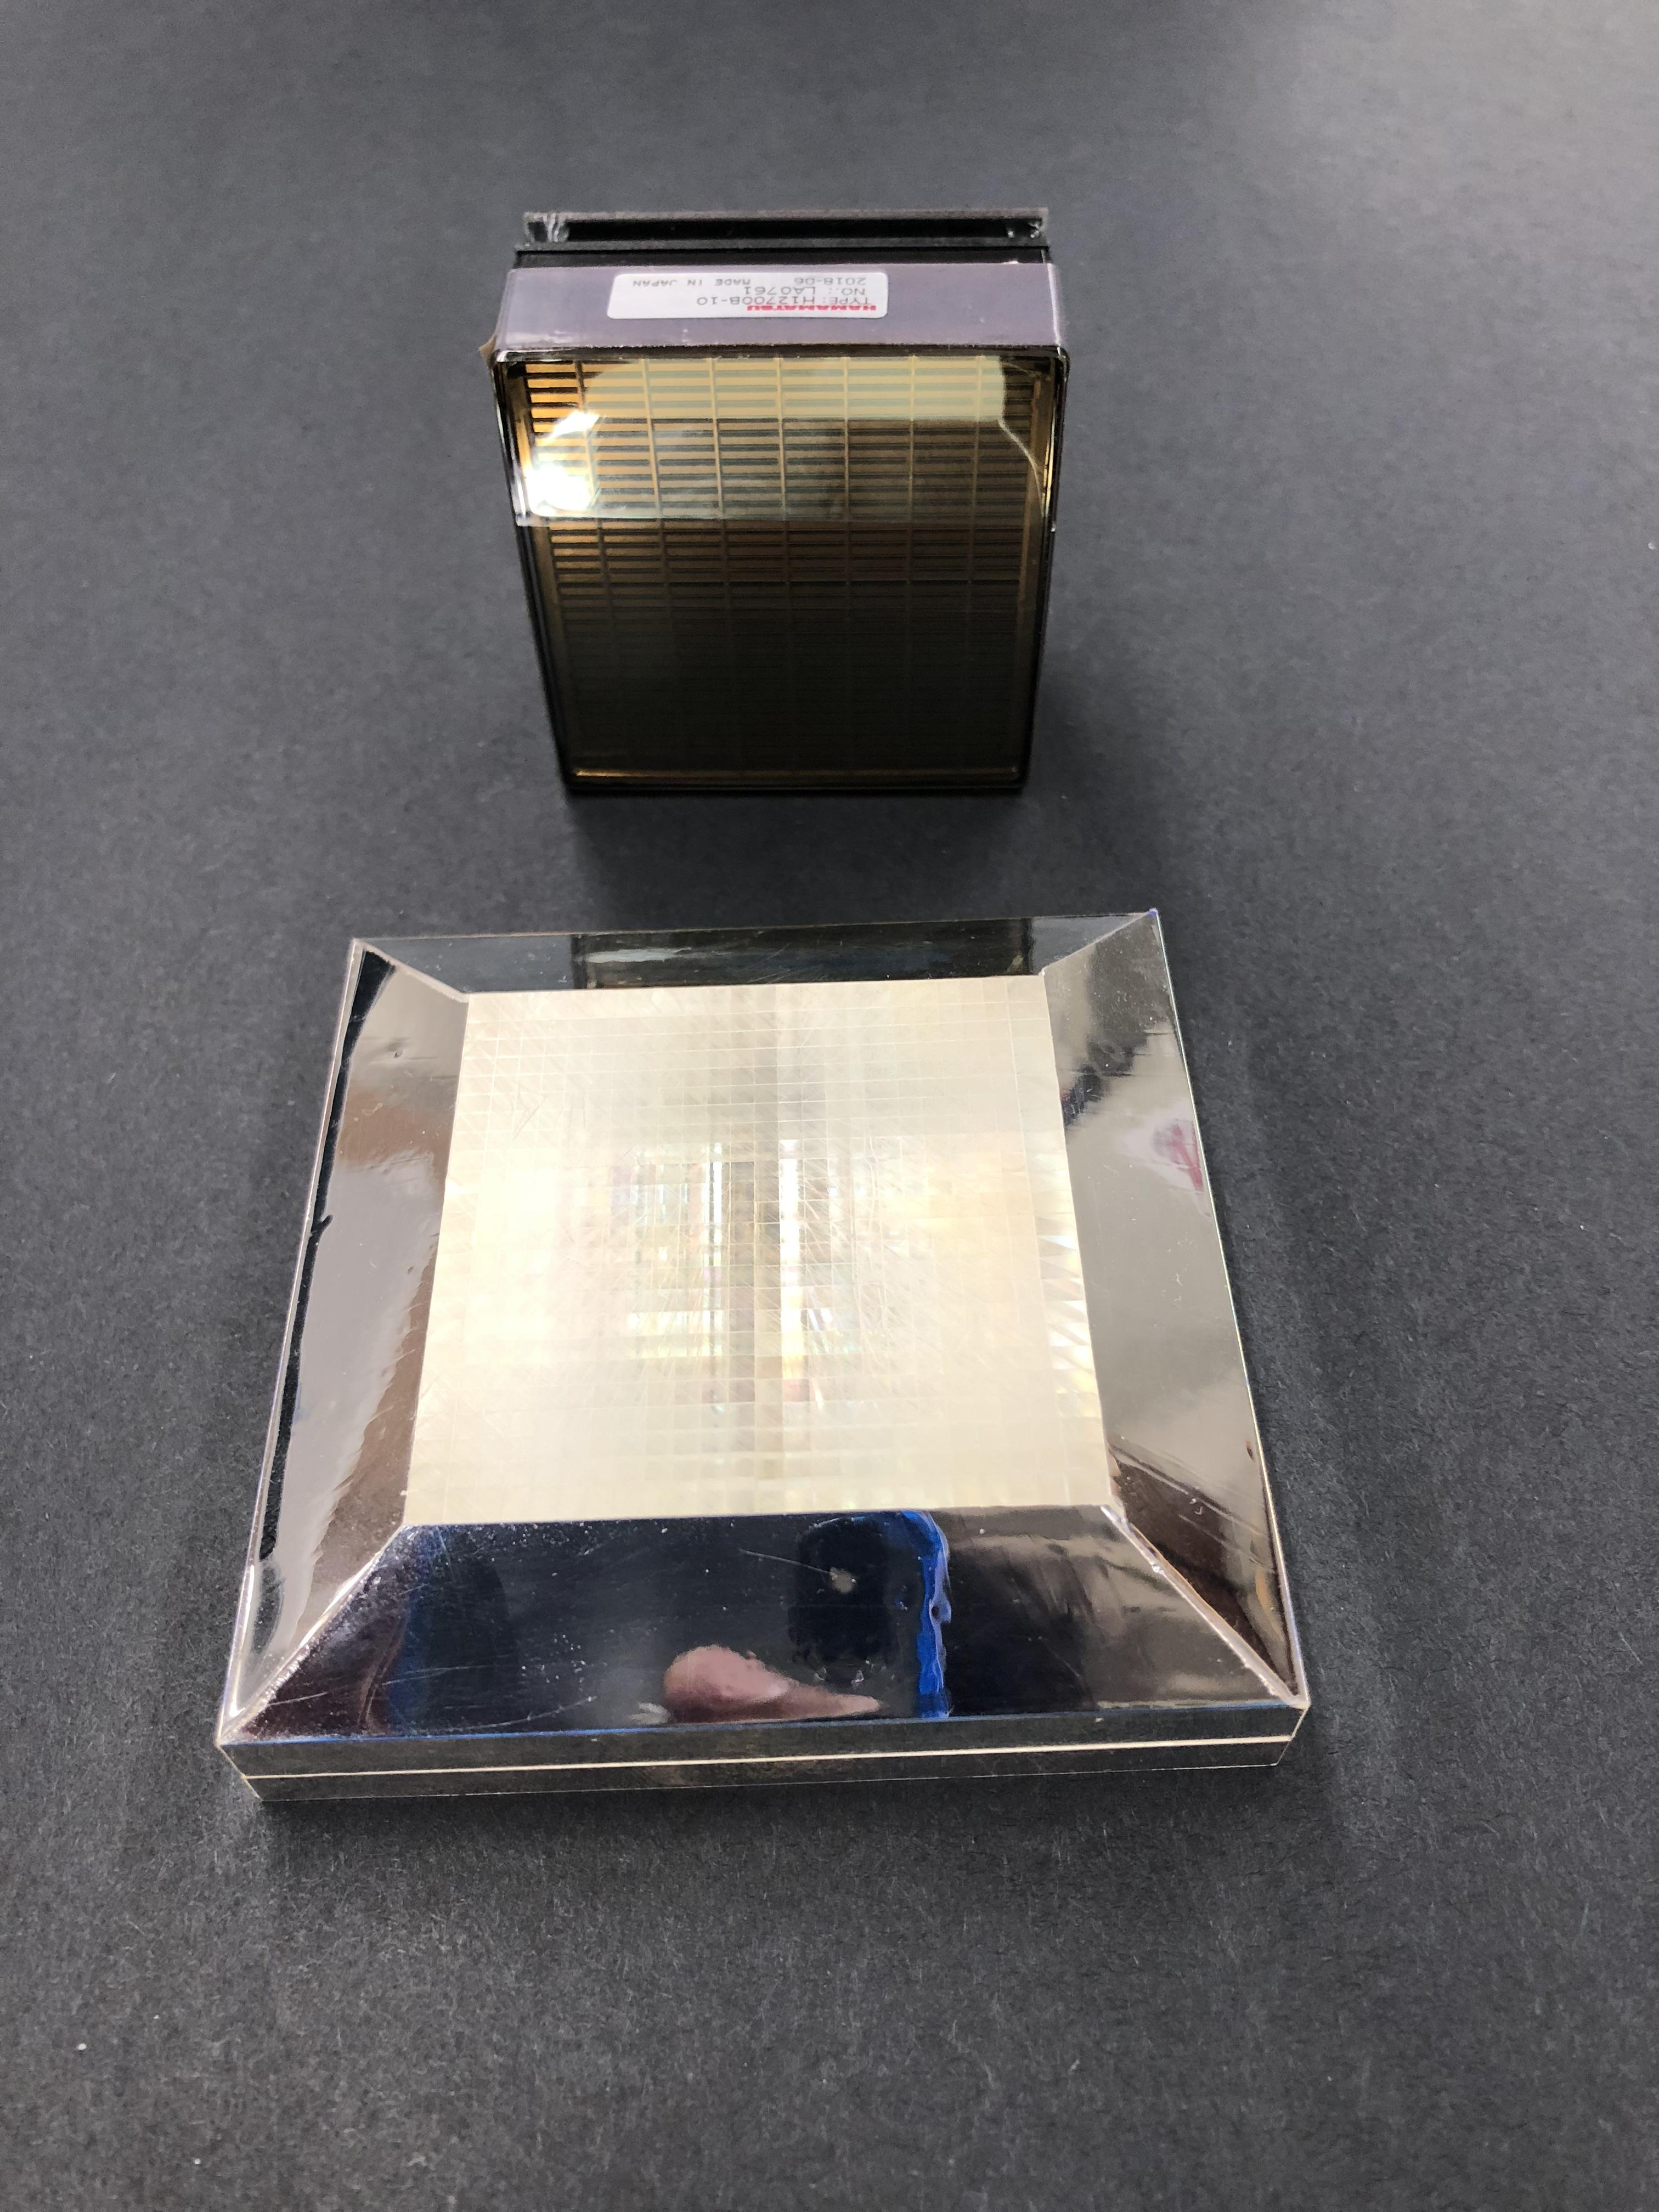
\includegraphics[width=7cm,height=7cm]{figures/new_yso_tapered_light_guide.jpg}
	\caption[The image above shows the crystal and light guide]{The image above shows the crystal and light guide combination, and the PSPMT used. The sides of the light guide are covered with ESR to ensure no light escaping.}
	\label{fig:yso_light_guidel}
\end{figure}
The sides of the connection are sealed with epoxy glue to ensure stronger support. This variant of the implantation detector has a larger area to capture a more divergent beam spot. \\
ToF is defined as follows:
\begin{equation}
\textit{ToF}=T\textsubscript{n}-T\textsubscript{$\beta$}
\end{equation}
where $T\textsubscript{n}$ is the time stamp of the neutron events recorded in VANDLE, and $T\textsubscript{$\beta$}$ is the time stamp of the beta events triggering YSO.

The energy of the neutrons can be deduced by the relation as follows:

\begin{equation}
E=\frac{1}{2} \times m_{n} \times  \frac{ L^2}{ ToF^{2}}
\end{equation}
where m\textsubscript{n} is the neutron mass, ToF is the Time of Flight, and L is the flight path. 

\begin{equation}
\frac{\Delta E}{E}  = \sqrt{\Bigg[\frac{2\Delta L}{L}\Bigg]^2 + \Bigg[\frac{2\Delta t}{t}\Bigg]^2}
\end{equation}

Where $\Delta L$ has contributions from the uncertainty in position measurement of electrons in YSO, and neutrons in VANDLE \citep{VANDLE}, $\Delta t$ is the timing-jitter, which is given by the root mean square of the timing resolution of YSO and VANDLE. $\Delta t$ in total encapsulates contributions from jitter induced by transit-time variance of photons in scintillator,  PSPMT response, digital electronics, and intermediate noise. 

\begin{figure}[h!]
	\centering
	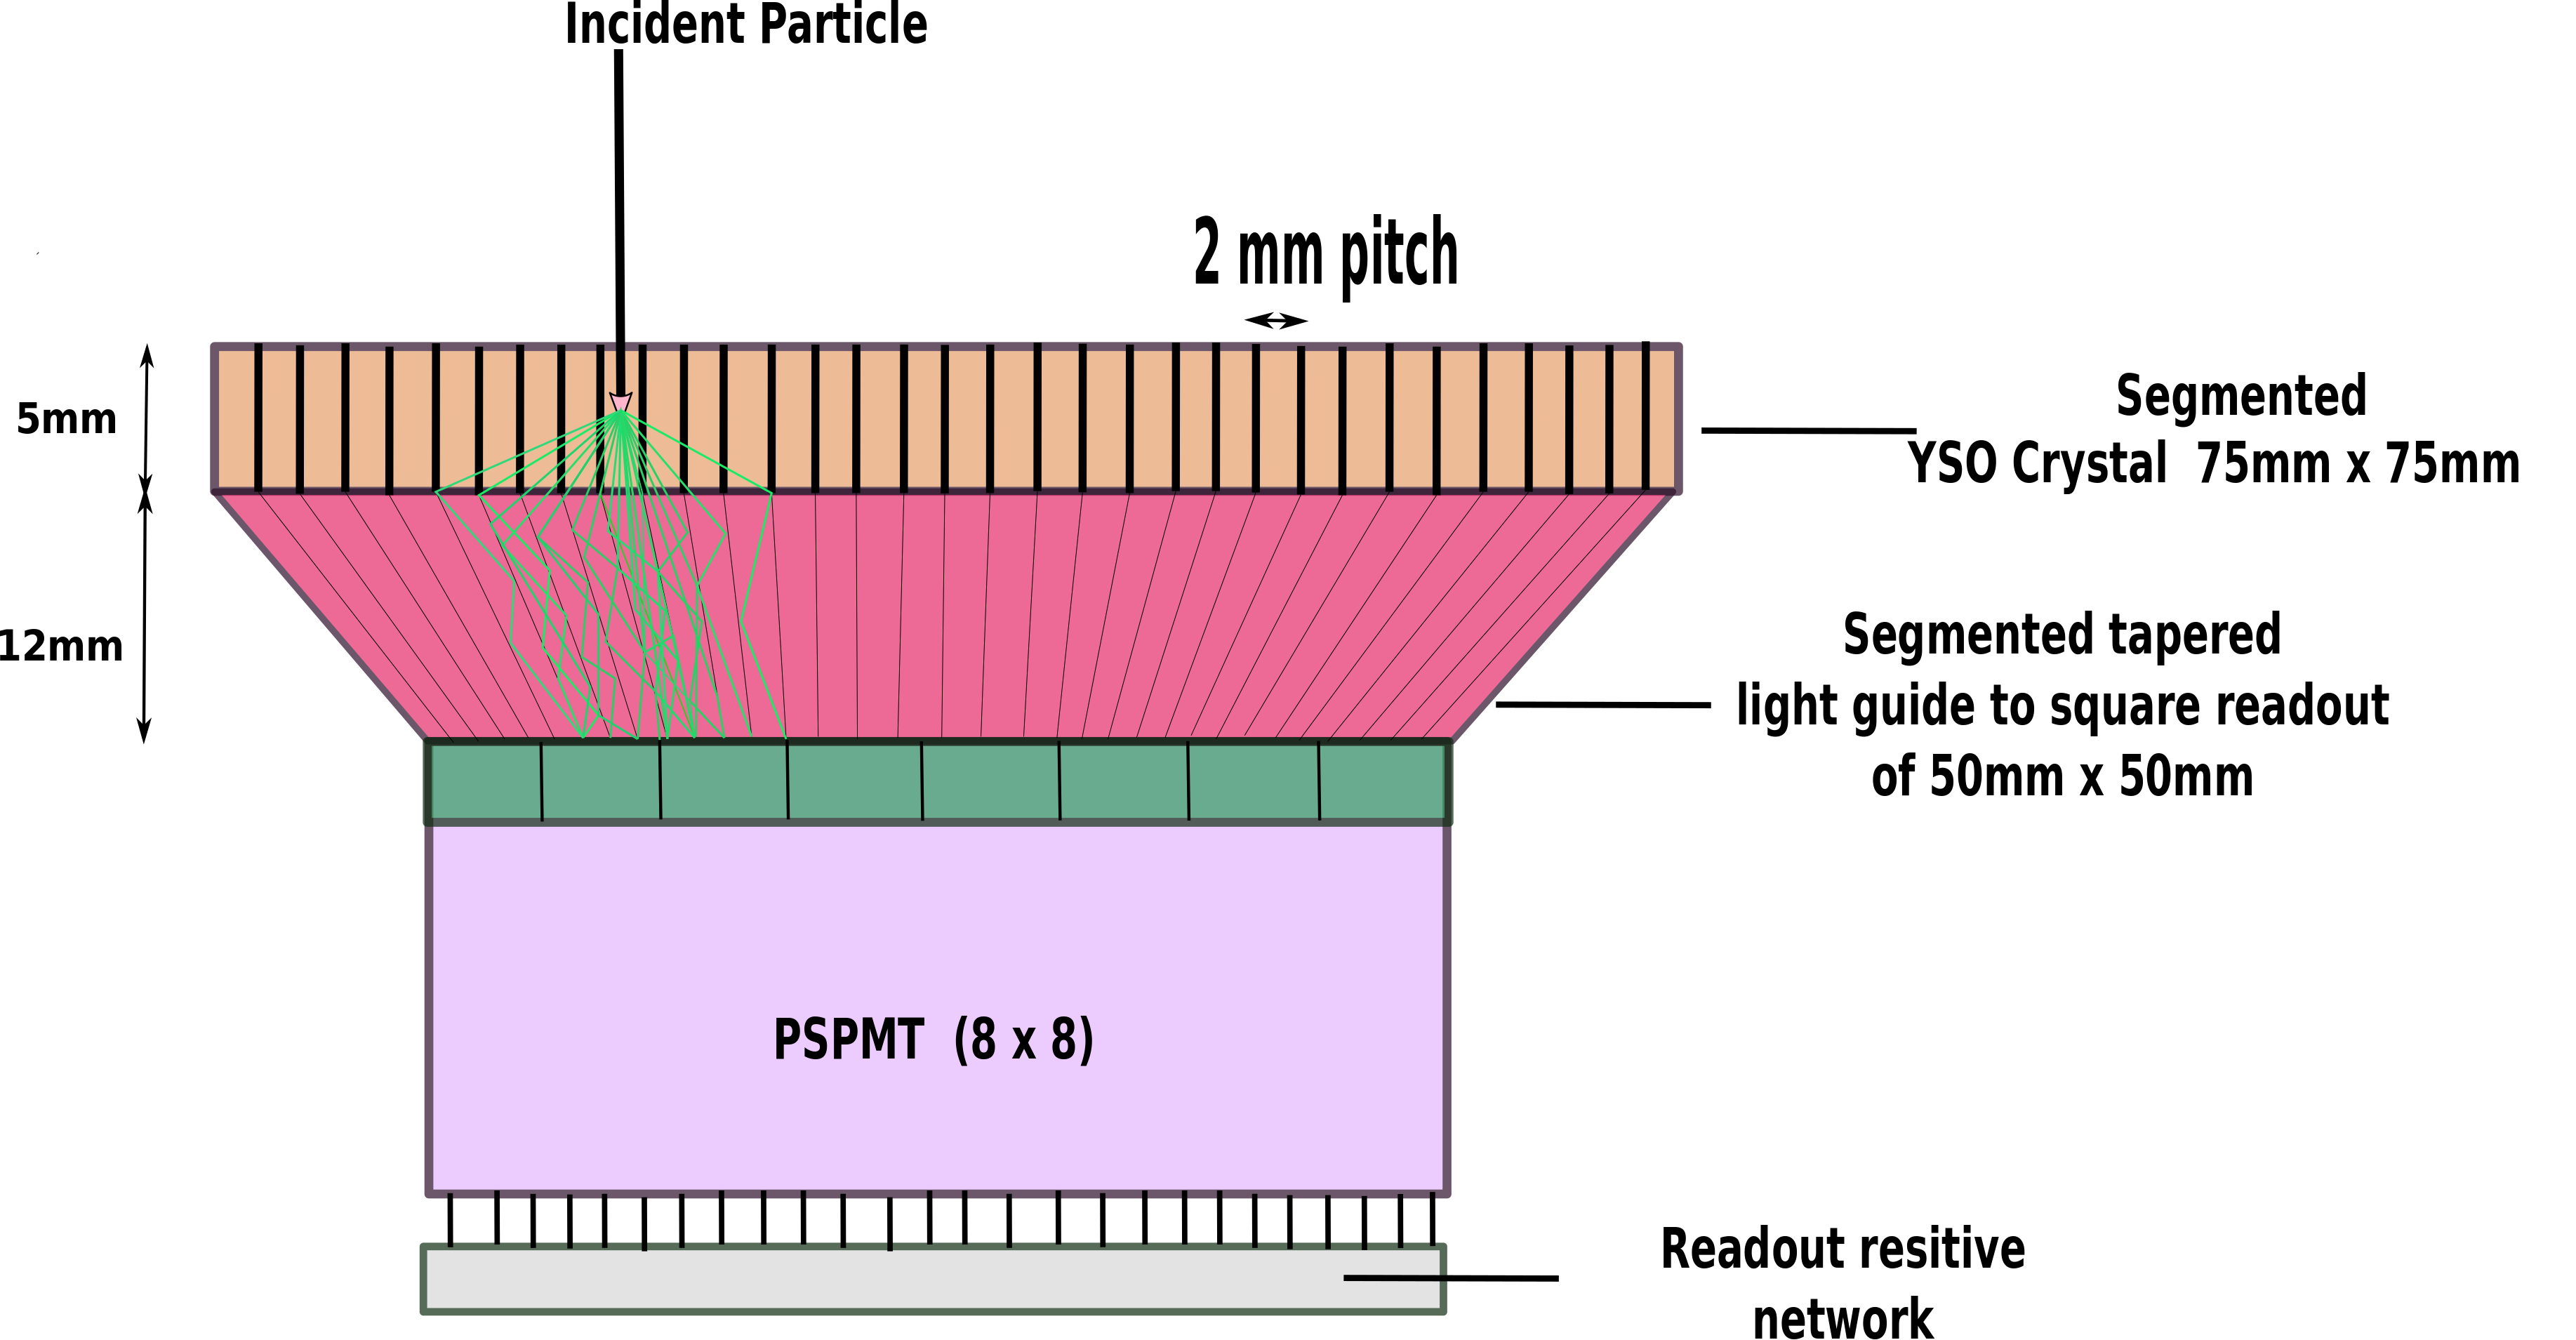
\includegraphics[width=14cm,height=8cm]{figures/yso_lightguide.png}
	\caption[A graphical depiction of the detector design]{A graphical depiction of the detector design, showing the placement of YSO crystal and light guide on PSPMT. Pathway of photons on its way to the sensor is through the light-guide.}
	\label{fig:yso_riken_2018}
\end{figure}
\newpage
\begin{figure}[h!]
	\centering
	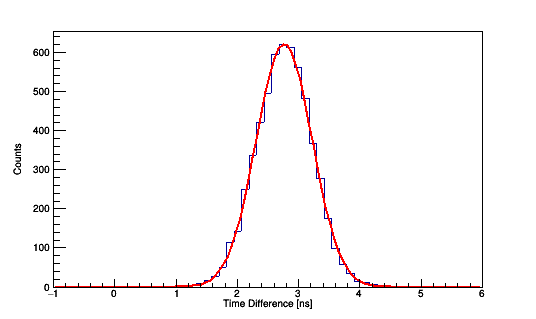
\includegraphics[width=12cm, height=8cm]{figures/YSO_timing.png}
	\caption[Time difference between the signals having gates]{Time difference between the signals having gates for energy above the Compton edge of \textsuperscript{60}Co. This configuration offers a timing resolution of $\sim$ 650 ps at 600 V. }
	\label{fig:time_resolution}
\end{figure}

From the above relation, uncertainty in the energy arise from the position and timing precision in both YSO and VANDLE. The position uncertainty for betas in YSO is of the order of mm, on the other, hand position uncertainty for neutrons is of the order of cm in VANDLE. Thus, VANDLE position uncertainty dominates in determining energy uncertainty. Timing resolution has equal contributions from both the detectors. A few tests were done to deduce the timing resolution of the YSO detector for signals representing various energy ranges. 

\begin{figure}[h!]
	\centering
	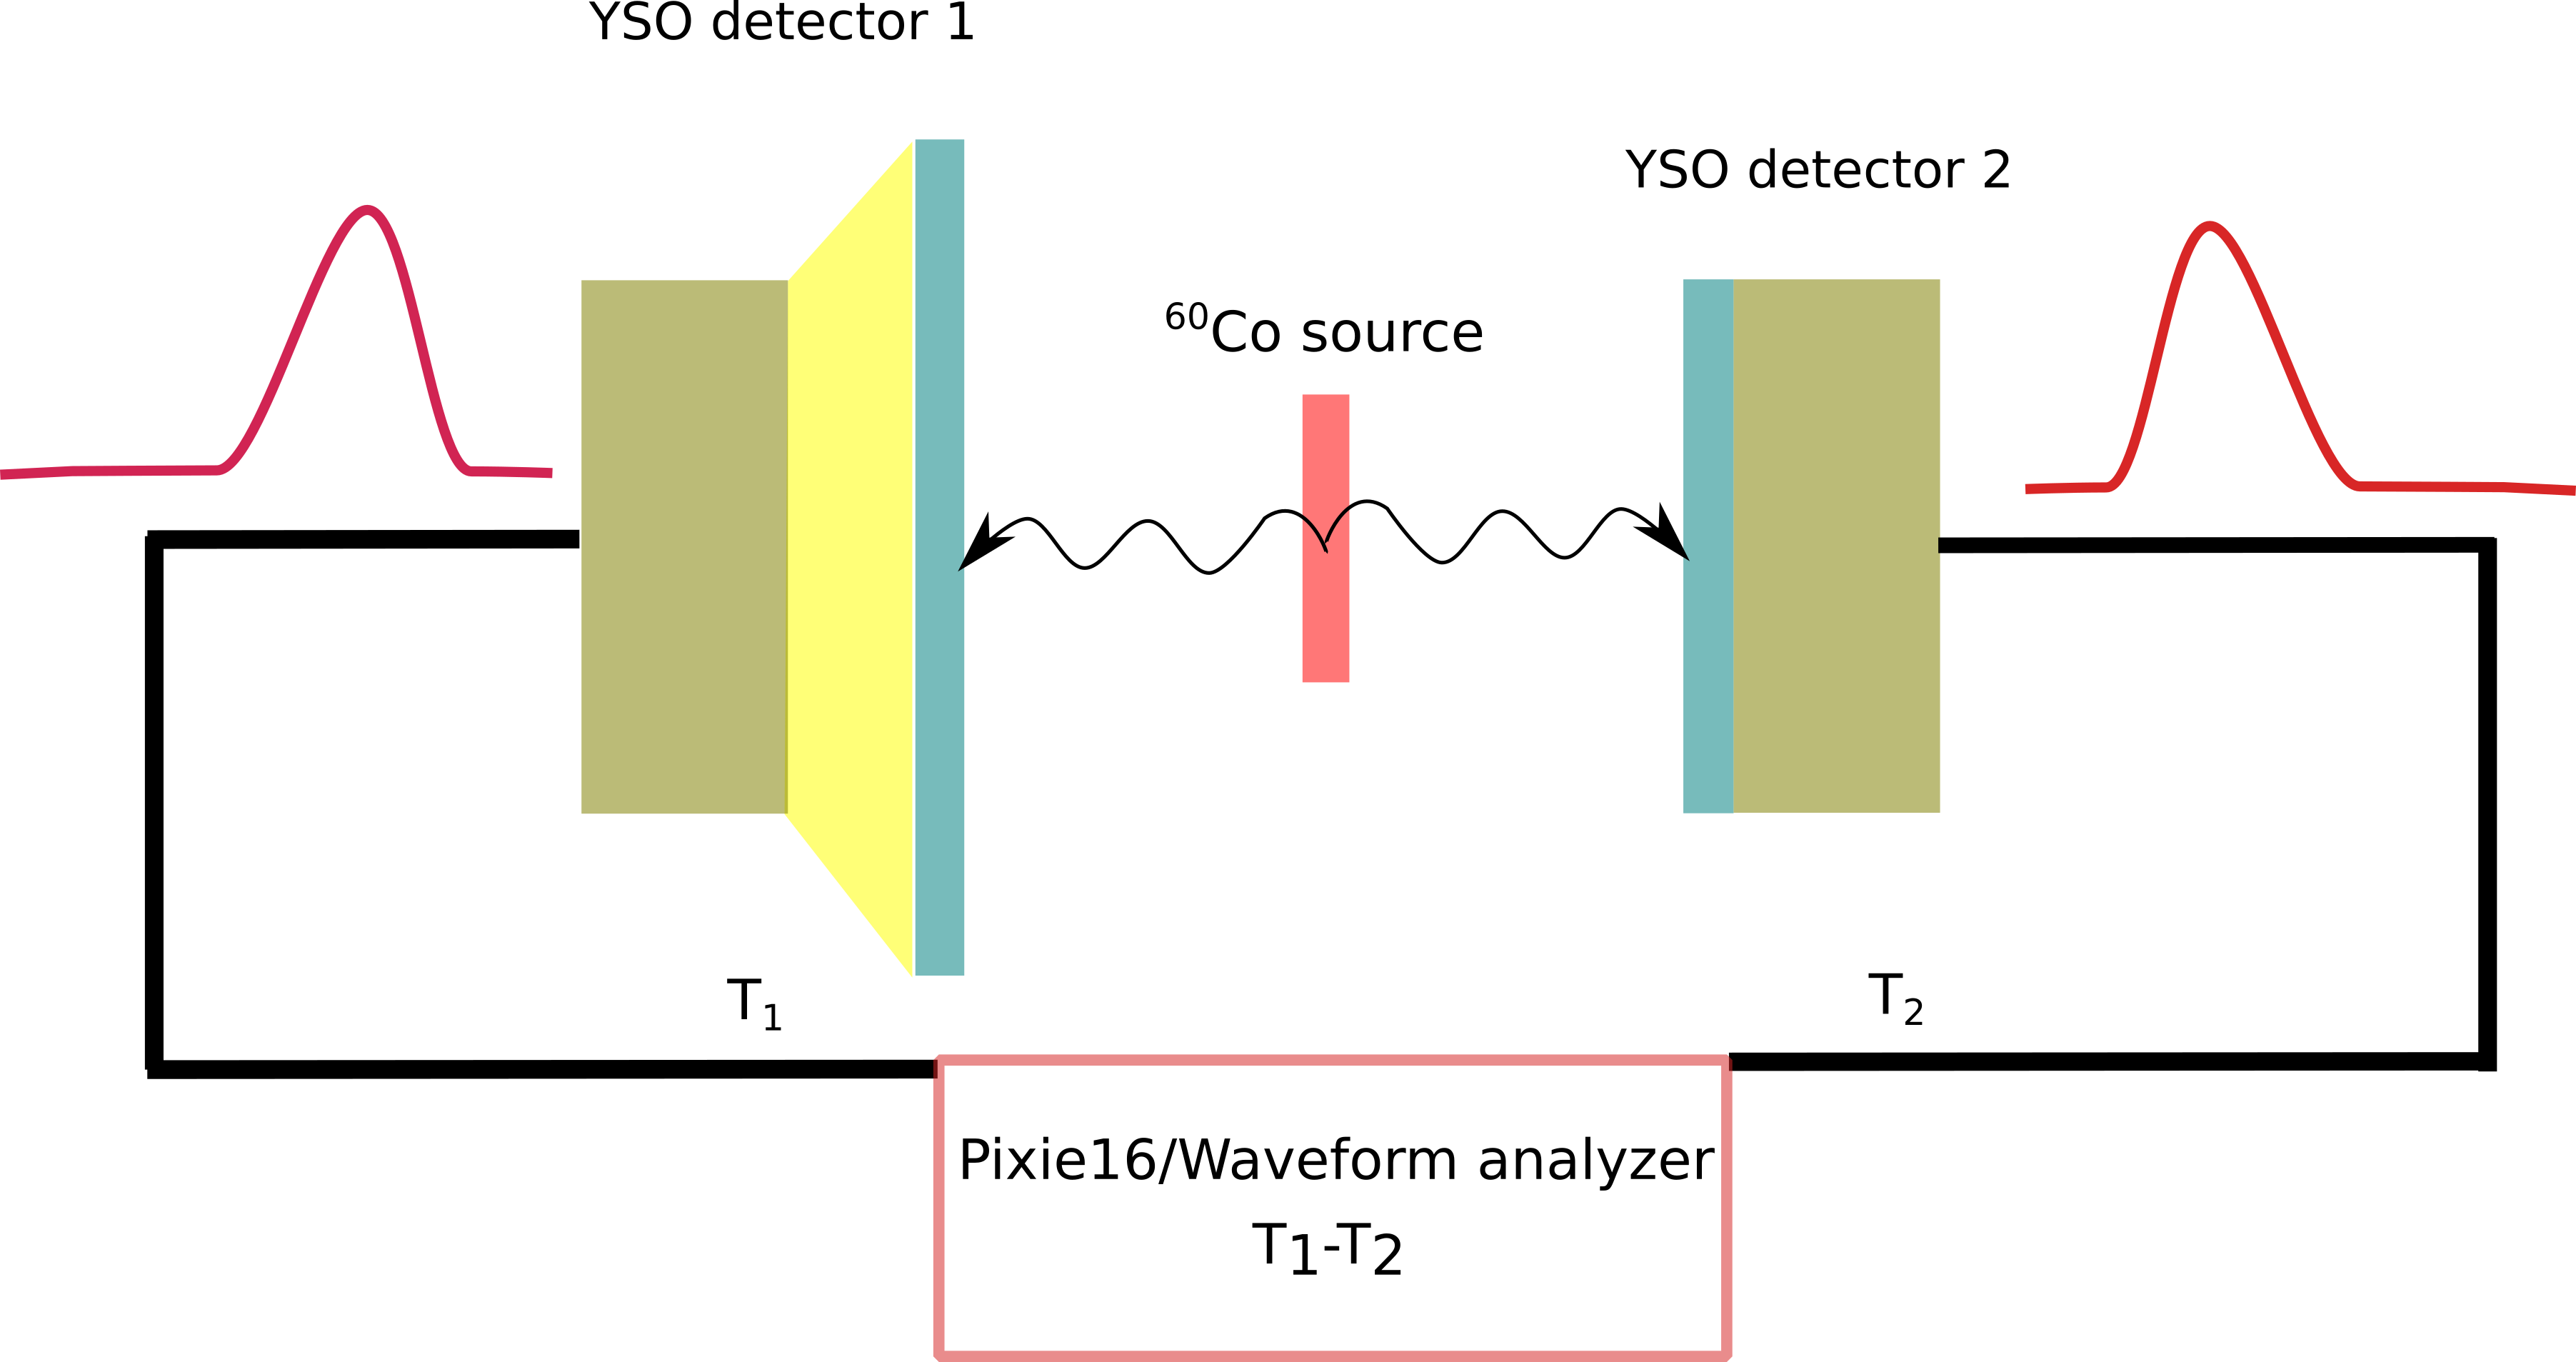
\includegraphics[width=16cm, height=10cm]{figures/yso_timing_test.png}
	\caption[]{Schematic of the setup for YSO timing measurement. }
	\label{fig:timing_measurement}
\end{figure}


The tests were done to ensure a good timing resolution for the actual experimental run. The criteria involved getting the time stamp of the same event in two similar YSO detectors using a \textsuperscript{60}Co source, and plotting the distribution of the difference in time, recorded in the two detectors. The distribution can be approximated to be Gaussian in nature. The Full-Width Half-Maximum (FWHM) of the distribution gives an estimate of the timing-resolution of both the detectors combined. Single detector resolution can be deduced assuming an equal uncertainty contribution for both the detectors. Scenarios with different biasing voltage were also explored. The detector, on average, has a timing resolution better than $\sim$ 600 ps for signals representing energy $\geq$ 1 MeV. Several other tests were performed to check the image quality, quality of coupling, and position resolution. 

\begin{figure}[h!]
	\centering
	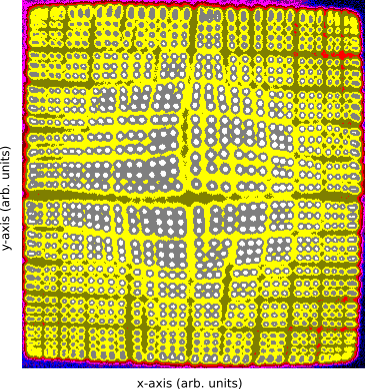
\includegraphics[width=9cm,height=9cm]{figures/yso_inkscape1.png}
	\caption[Flat-field image produced using \textsuperscript{137}Cs source on]{Flat-field image produced using \textsuperscript{137}Cs source on \textit{x-y} plane (arbitrary scaling) showing each pixel well-illuminated. The crystal is 7 cm $\times$ 7 cm with each pixel having dimension 2mm $\times$ 2mm. The gaps are present in the image because of the light guide being constructed out of four different sections and joined together. The pixels on the corner are more crowded because of the relatively more tapering of the light guide along the z-axis for the edges than for the center.}
	\label{fig:flood_field_image}
\end{figure}
\subsubsection{Range Distribution of Ions and Electrons in YSO}


/*Insert the test images gain for example for Sr90 and Cs137*/
/*Also insert the individual signals*/
/**/

Exotic isotopes present in the cocktail beam are highly energetic having the energy of the order of GeV. An estimate of the range of these ions in YSO crystal is important from the point of view of the experiment, where collecting ample statistics is of prime concern. These estimates are also important for detector design, helpful in choosing the right thickness of the scintillating material. \textbf{LISE++} \citep{lise} is a software that has been developed to calculate the transmission and yields of fragments produced and collected in a spectrometer. The LISE++ code may be applied at medium-energy and high-energy facilities (fragment- and recoil-separators with electrostatic and magnetic selections). In a number of facilities, like A1900 and S800 at NSCL, LISE3, SISSI/LISE3, and SPEG at GANIL, FRS and SuperFRS at GSI,  RIPS and BigRIPS at RIKEN, based on the separation of projectile-like and fission fragments,  fusion residues are included or might be easily added to the existing optical configuration files. The range estimates of ions produced can be deduced for any material by providing chemical properties of the material to LISE.
\newpage
\begin{figure}[h]
	\centering
	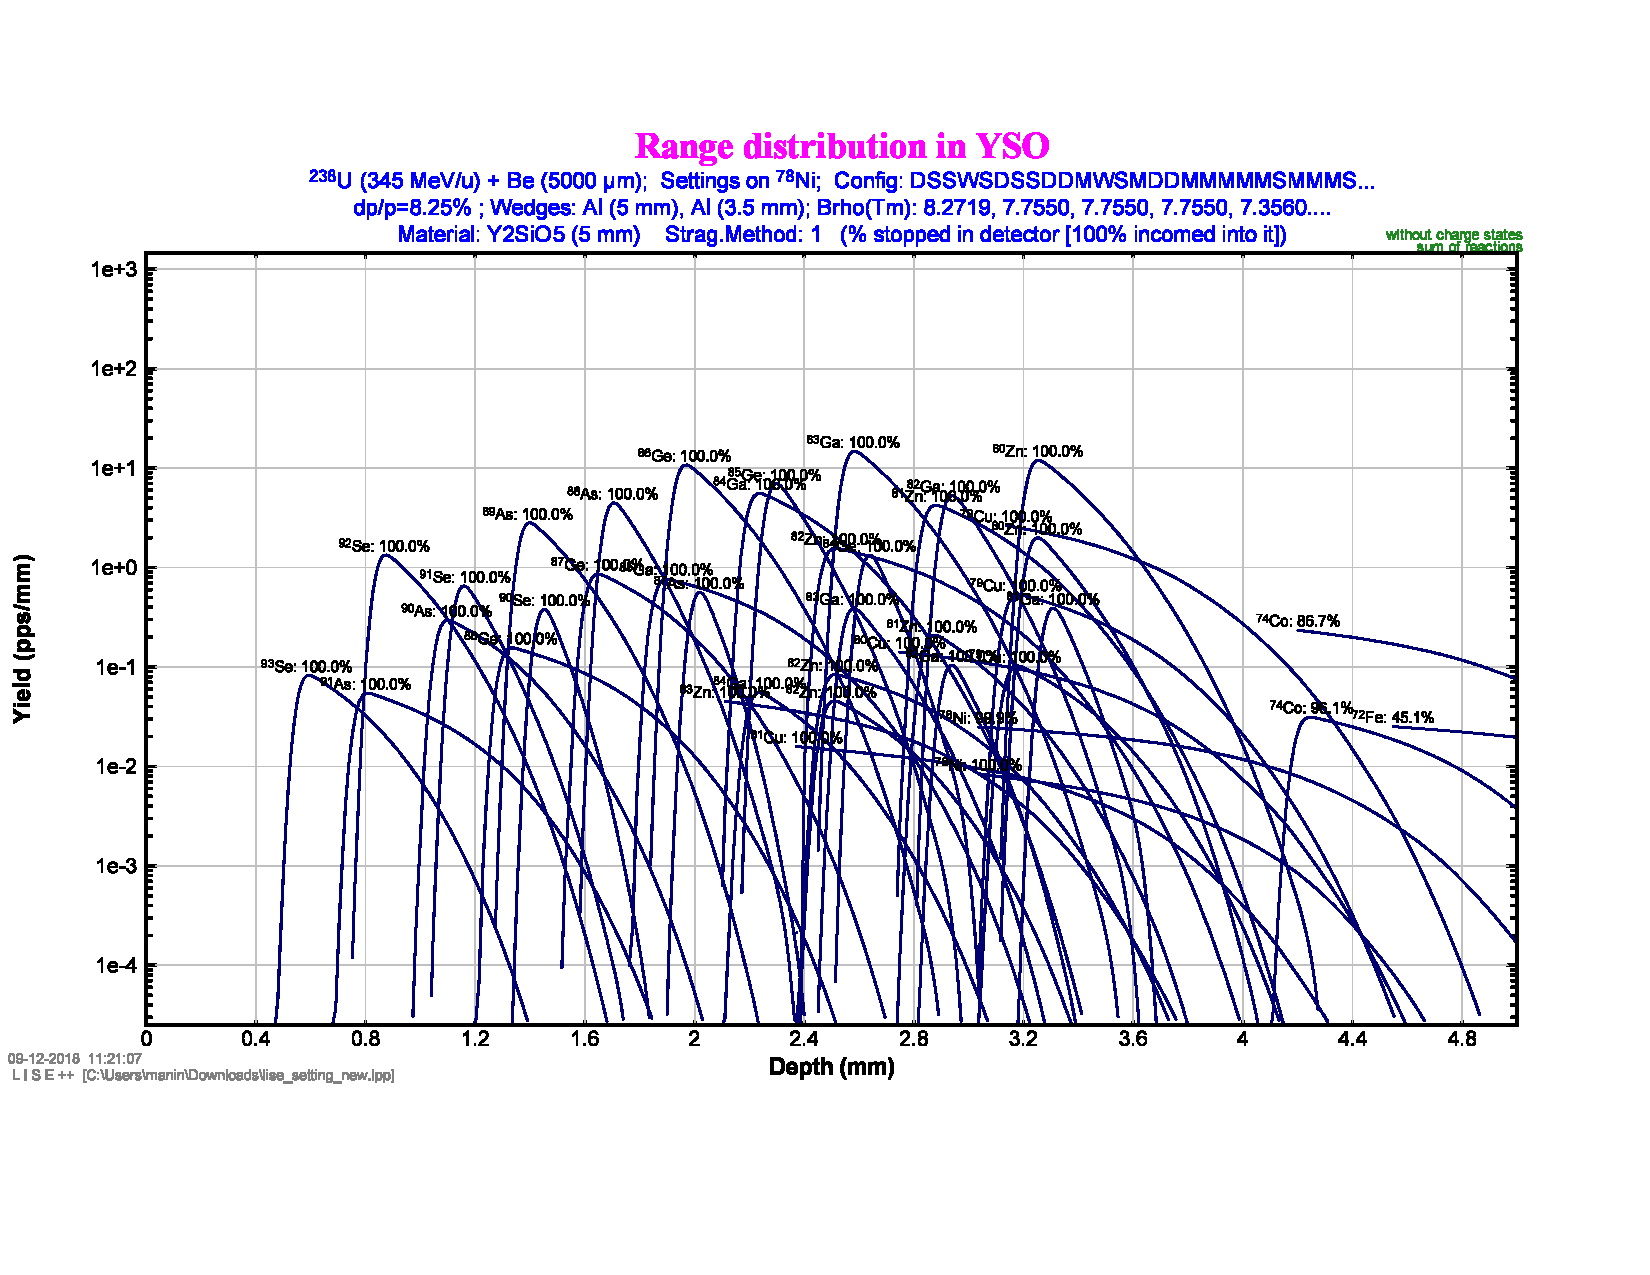
\includegraphics[height=16cm, width=17cm]{figures/yso_lise_snapshot-rotated.pdf}
	\caption[Range distribution of various ions in YSO]{Range distribution of various ions in YSO. The configuration for the calculations is reminiscent of the setup available at RIBF, RIKEN. The heaviest ions are implanted shallower with full absorption, lighter ions have relatively deeper implantation, requiring proper energy-degraders for total stoppage in YSO. }
	\label{fig:ionrangeyso}
\end{figure}

Electrons generated followed by the $\beta^{-}$-decay of these radioactive ions can have energy as low as a few keV or as high as a few MeV. Information about the range of electrons of various energy is also vital from the ion-$\beta$ correlation perspective. It is helpful in designing and optimizing the position gates around implant positions. These range estimates were produced using on internet program \textbf{ESTAR} \citep{estar}. Details about chemical composition and density are the input parameters to the program. The program calculates  stopping power, density effect parameters, range, and radiation yield tables for electrons in various materials.

\begin{figure}[h!]
	\centering
	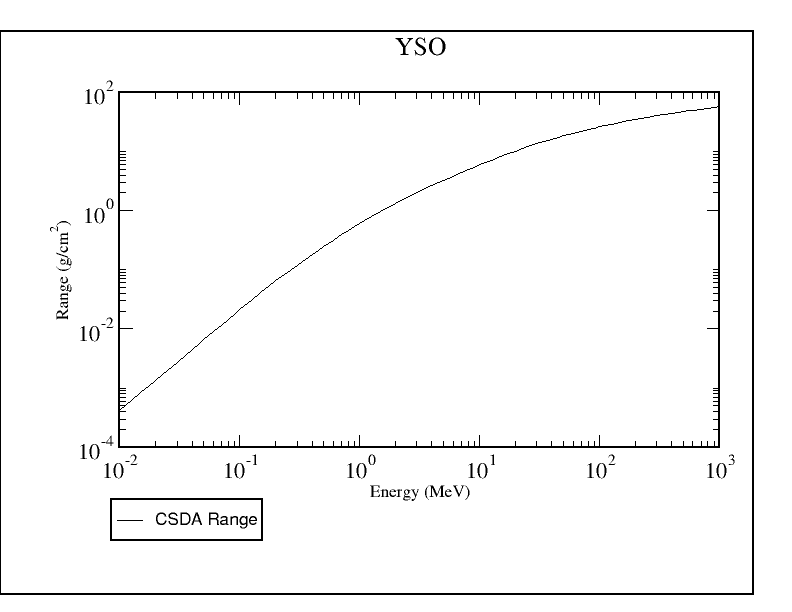
\includegraphics[width=10cm,height=8cm]{figures/yso_electrons_range.png}
	\caption[Continuous slowing down approximation range (CSDA)]{Continuous slowing down approximation range (CSDA) of electrons in YSO computed using ESTAR.}
	\label{fig:electron_range_yso}
\end{figure}

    \chapter{Experiment} \label{ch:experiment}

\section{Radioactive Ion Beam Factory(RIBF) at RIKEN}

\begin{figure}[h!]
\centering
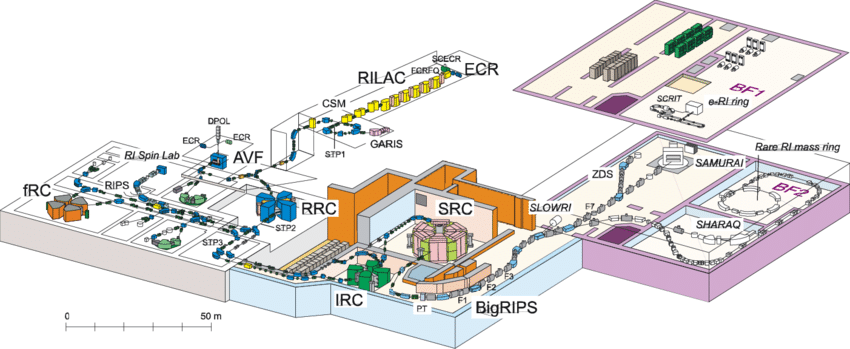
\includegraphics[width=15cm, height=11cm]{figures/Layout-of-the-RIKEN-RI-Beam-Factory.png}
\caption[Layout of the RIBF showing various accelerators]{Layout of the RIBF showing various accelerators and the BigRIPS ion separator \citep{rikenasc}. }
\end{figure}
The RIBF is world-class fragmentation ion beam facility. It is part of physics division at RIKEN, Japan. The facility consists of a 22 year old facility(since 1986) and a new facility which has been completed recently. The old facility has the heavy-ion accelerator complex consisting of a K540-MeV ring cyclotron (RRC) and its two injectors: a variable-frequency heavy-ion linac (RILAC) and a K70-MeV AVF cyclotron (AVF). These accelerators have been providing a lot of users in various research fields with the world’s most intense ion beams over the whole range of elements. The RILAC provides a heavy-ion beam with energy up to 6 MeV/nucleon. The AVF provides protons up to 14 MeV and Ca ions up to 5.6MeV/nucleon. The RRC can provide protons up to 210 MeV, heavy ions such as C, O and Ne ions up to 135MeV/nucleon, Ar ions up to 95 MeV/nucleon and Bi ions up to 15 MeV/nucleon. Moreover, the projectile-fragment separator at the RRC (RIPS) provides the world's most intense low-atomic-mass (\textless 60) RI beams.

The RIBF has very recently added new dimensions to the facility's capabilities: a new high-power heavy-ion booster system consisting of three ring cyclotrons with K=570 MeV (fixed frequency, fRC), 980 MeV (intermediate stage, IRC) and 2500 MeV (superconducting, SRC), respectively, can boost energies of the output beams from the RRC up to 440 MeV/nucleon for light ions and 350 MeV/nucleon for very heavy ions. The goal of the available intensity is set to be 1 p$\mu$A, which is limited due to presently planned radiation shielding power around a primary-beam dump. The superconducting isotope separator, BigRIPS, converts these energetic heavy-ion beams into intense RI beams via the projectile fragmentation of stable ions or the in-flight fission of uranium ions. The combination of the SRC and the BigRIPS expands our nuclear world on the nuclear chart into \textit{terra incognita}. 

\begin{figure}[h!]
\centering
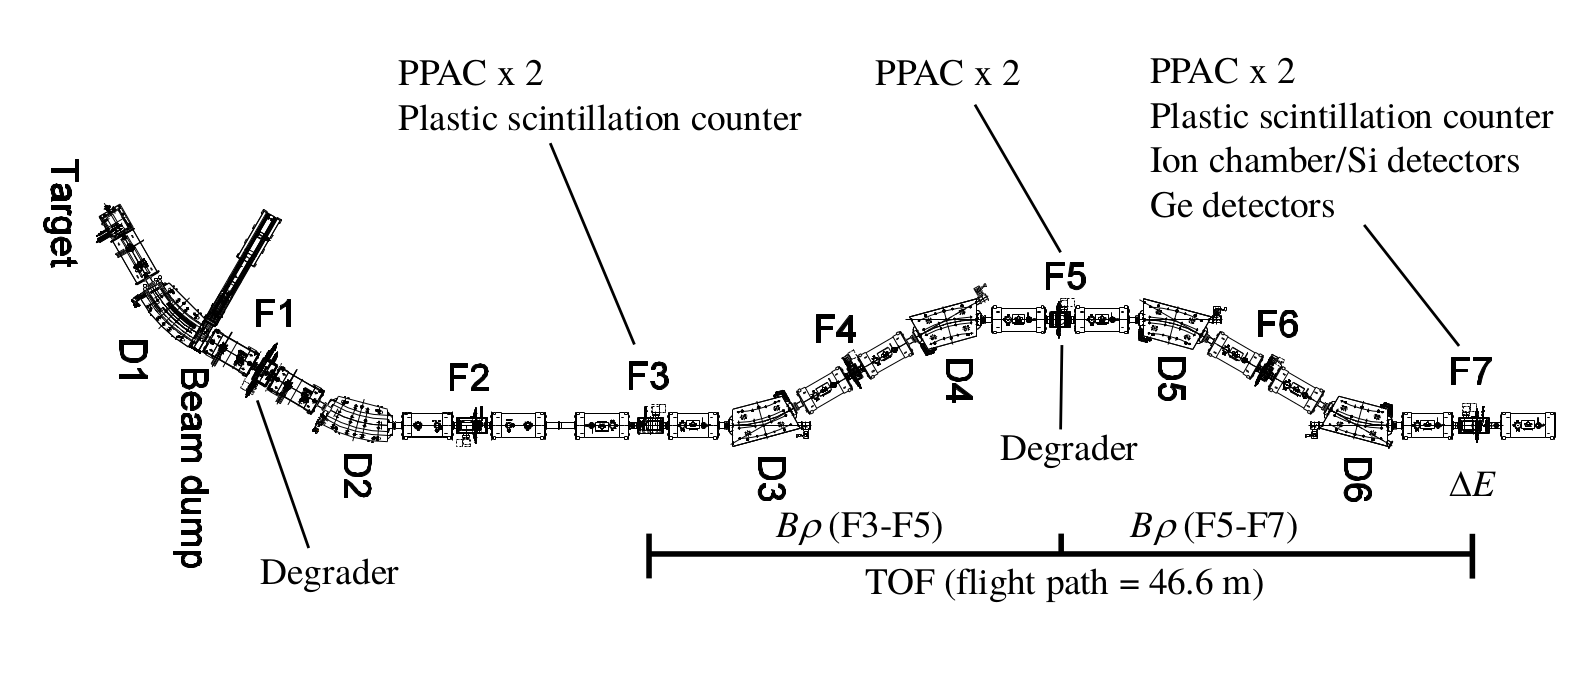
\includegraphics[width=19cm, height=11cm, angle=90]{figures/bigrips.png}
\caption[Schematic diagram of the BigRIPS separator]{Schematic diagram of the BigRIPS separator at RIBF. The first stage includes the components from the production target (F0) to F2, while the second stage spans those from F3 to F7 \citep{FUKUDA2013323}.}
\end{figure}

BigRIPS is an in-flight RI beam separator available at RIBF for the production of intense RI beams with a wide range of masses and isospin. The characteristic features of the BigRIPS separator are large ion-optical acceptances and a two-stage structure. The angular acceptances are $\pm$40 mrad horizontally and $\pm$50 mrad vertically, and the momentum acceptance is
$\pm$3 $\%$, allowing efficient collection of fragments produced by not only projectile fragmentation but also in-flight fission of a
\textsuperscript{238}U beam. The large acceptances are achieved by the use of superconducting quadrupoles with large apertures. The two-stage structure allows delivery of tagged RI beams and two-stage isotope separation. The first stage of the BigRIPS separator is used for production, collection, and separation of RI beams with an energy degrader, while particle identification of RI beams (separator-spectrometer mode) and/or further isotope separation with another energy degrader (separator-separator mode) are performed in the second stage. The particle identification is based on the TOF-B$\rho$ -$\Delta$E method, in which the time of flight (TOF), magnetic rigidity (B$\rho$ ), and energy loss ($\Delta$E) are measured to deduce the atomic number (Z) and the mass-to-charge ratio (A/Q) of RI beams. Such in-flight particle identification is an essential requirement for delivering tagged RI beams, making it possible to perform various types of experiments including secondary reaction measurements. Since the total kinetic energy is not measured in this scheme, and consequently A and Q cannot be determined independently, the resolution in A/Q must be high enough to identify the charge state Q of RI beams. Furthermore, the flight path is fairly long (46.6 m), so that the TOF value can be determined with fairly high resolution.



\subsection{YSO implementation in BRIKEN experiment}

The YSO detector was used for the first time at RIBF, RIKEN for two consecutive experiments. It was implemented as a part of the BRIKEN \citep{BRIKEN} neutron counter already present at the facility. The YSO detector was used as one of the implant detectors along with WAS3ABI and AIDA. The PSPMT of the detector was optimized to operate at a biasing voltage of 575 V to get the desired dynamic range for the ions, and the betas. The experiments involved accelerating \textsuperscript{238}U upto 345 MeV/nucleon with a charge state of (86+) which is the primary beam, followed by hitting a 4 mm thick rotating target of \textsuperscript{9}Be.
\begin{figure}[h]
    \centering
    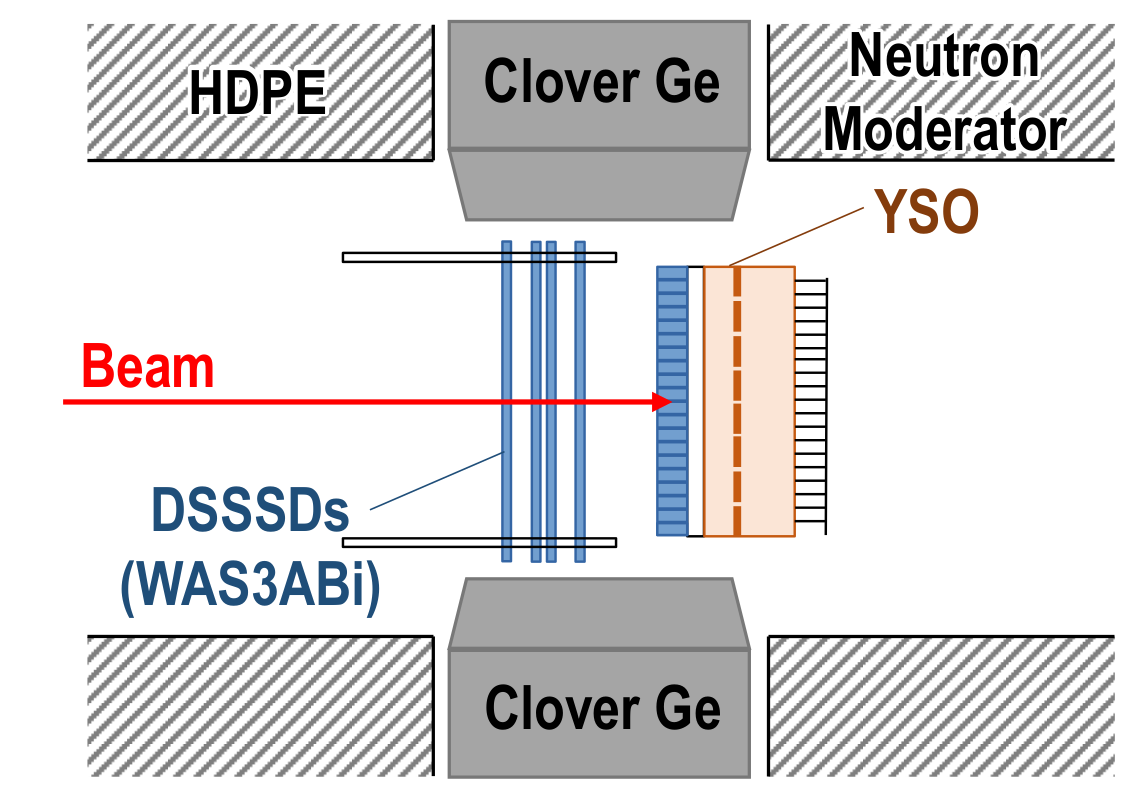
\includegraphics[width=10cm,height=8cm]{figures/experimental_setup.png}
    \caption[A diagram showing the instrumental setup for the]{A diagram showing the instrumental setup for the experiment as viewed from above. WAS3ABi and YSO are placed in a cavity at the center of BRIKEN neutron detector, approximately 2 cm apart. This position geometrically ensures detection of maximum possible neutrons (prompt and delayed) by the neutron counter. The High Density Polyethylene (HDPE) is used to moderate energetic delayed neutrons, advancing them in a region of high interaction cross-section with the \textsuperscript{3}He tubes comprising the BRIKEN neutron counter. Two High purity germanium clover detectors were employed to record the $\beta$-correlated $\gamma$-rays.}
    \label{fig:experimental}
\end{figure} 
The reaction leads to the synthesis of a gamut of exotic isotopes which are tagged and separated by BigRIPS facility on an event by event basis. This tagged  secondary beam of ions provided by the BigRIPS facility was implanted onto the detector with a particular combination of aluminum degraders, required to monitor the energy and range of ions. The first experiment had a secondary beam centered around \textsuperscript{82}Cu, and the second experiment itself involved
two mass settings. The first setting involved nuclei around \textsuperscript{115}Nb and the second setting provided nuclei centered around \textsuperscript{100}Br. 
The five signals (four positions and one energy) from the detector were split and used with different gain settings. One set of signals was devoted to implant position and energy measurements with no amplification. The other set was used for calculating the energy and position of the betas, with an amplification $\sim$ 10 for obtaining a good signal-to-noise ratio leading to better estimates of energy as well as position in the \textit{x-y} plane of the detector.


\begin{figure}[h!]
    \centering
    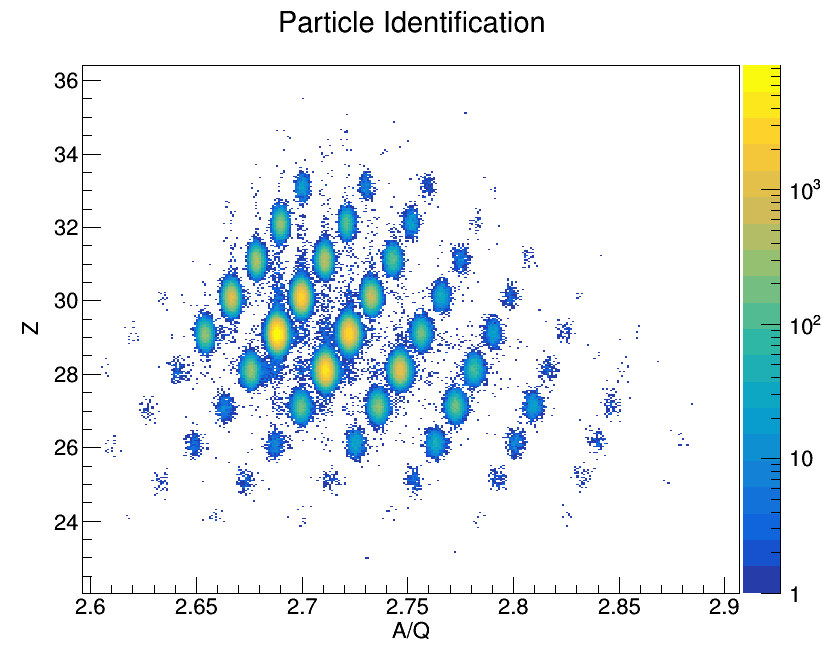
\includegraphics[width=10cm, height=8cm]{figures/yso_pid_2.png}
    \caption[Particle identification plot for ions stopped in YSO]{Particle identification plot for ions stopped in YSO. This information is provided by the BigRIPS facility and is important for ion-specific analysis.}
    \label{fig:particleidentification}
\end{figure}

\subsubsection{Ion-$\beta$ Correlations}
The essential purpose of the implantation detector is to establish the correlations between implanted ions and the corresponding $\beta$-decay electrons. These correlations are implemented by using a position-gate around the position of the implanted ion in the \textit{x-y} plane. The gate is optimized to achieve a high beta efficiency, thus maximum signal-to-noise ratio. 

The correlations are used in calculating half-lives of various isotopes and to further investigate the decay chains involving neutrons. The correlations were verified by calculating the half-lives of the known isotopes. Figure \ref{fig:ysocorrelations} shows the correlations between $\beta$ and implantation events. The correlation is manifested in the form of a hot-spot in the implant image in the vicinity of the $\beta$-event on the image scale. 

\begin{figure}[h!]
    \centering
    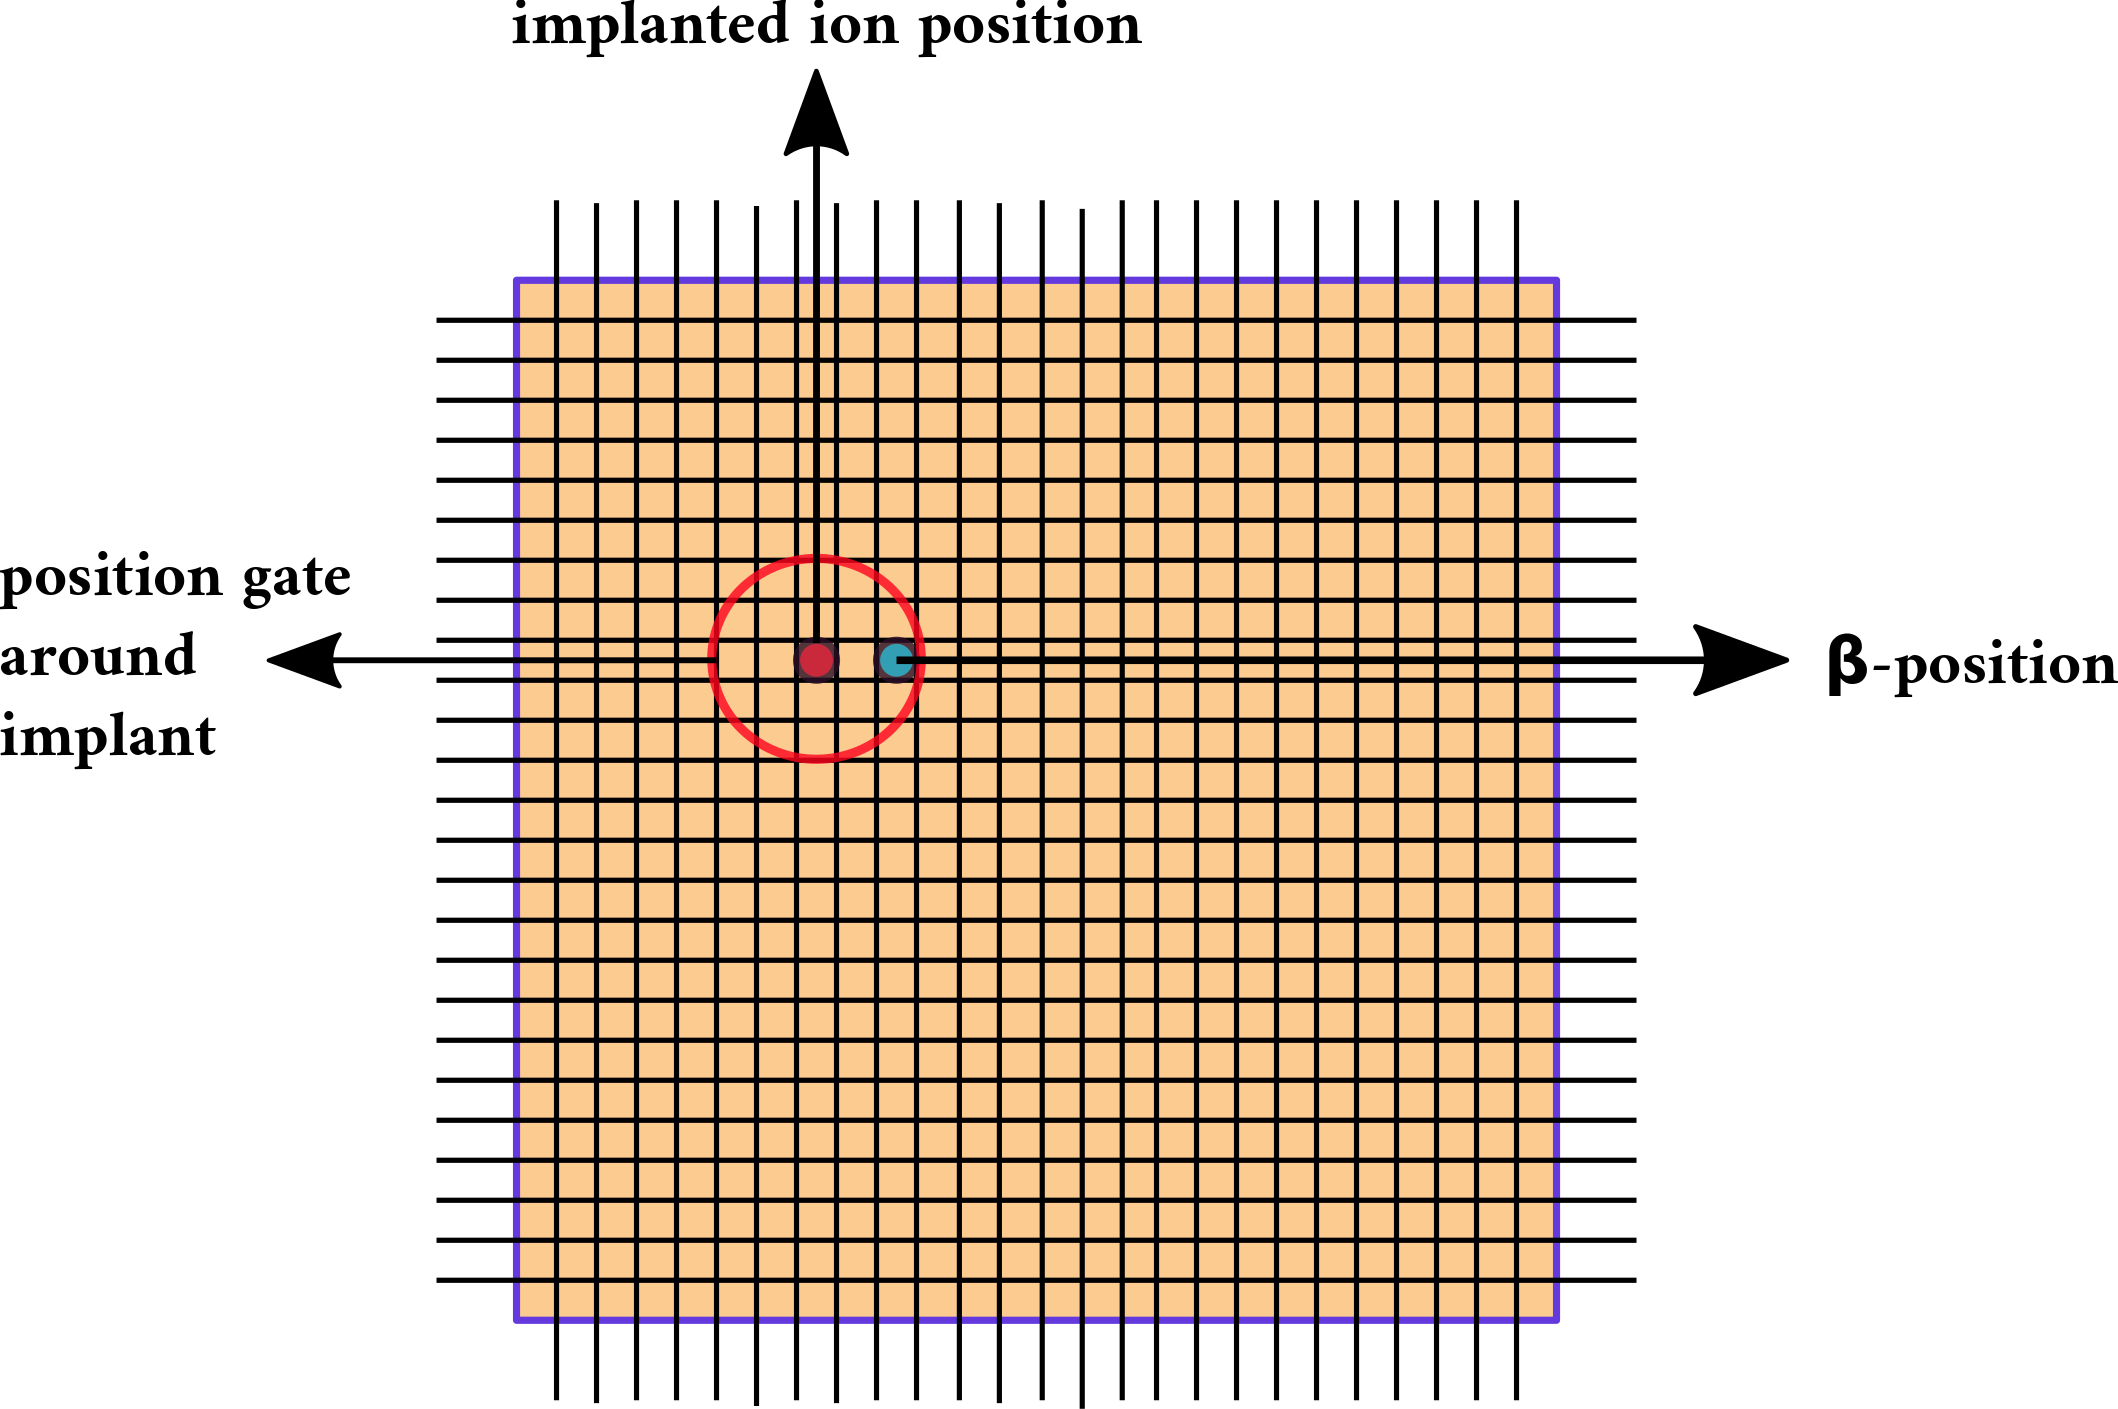
\includegraphics[width=12cm,height=8cm]{figures/pastedImage.png}
    \caption[A graphical representation of the algorithm devised to identify ion-beta]{A graphical representation of the algorithm devised to identify ion-beta correlations, showing a valid association. The diagram shows ion and beta position with red and blue shaded circles, respectively.}
    \label{fig:ion_beta_correlations}
\end{figure}

\begin{figure}[h!]
    \centering
    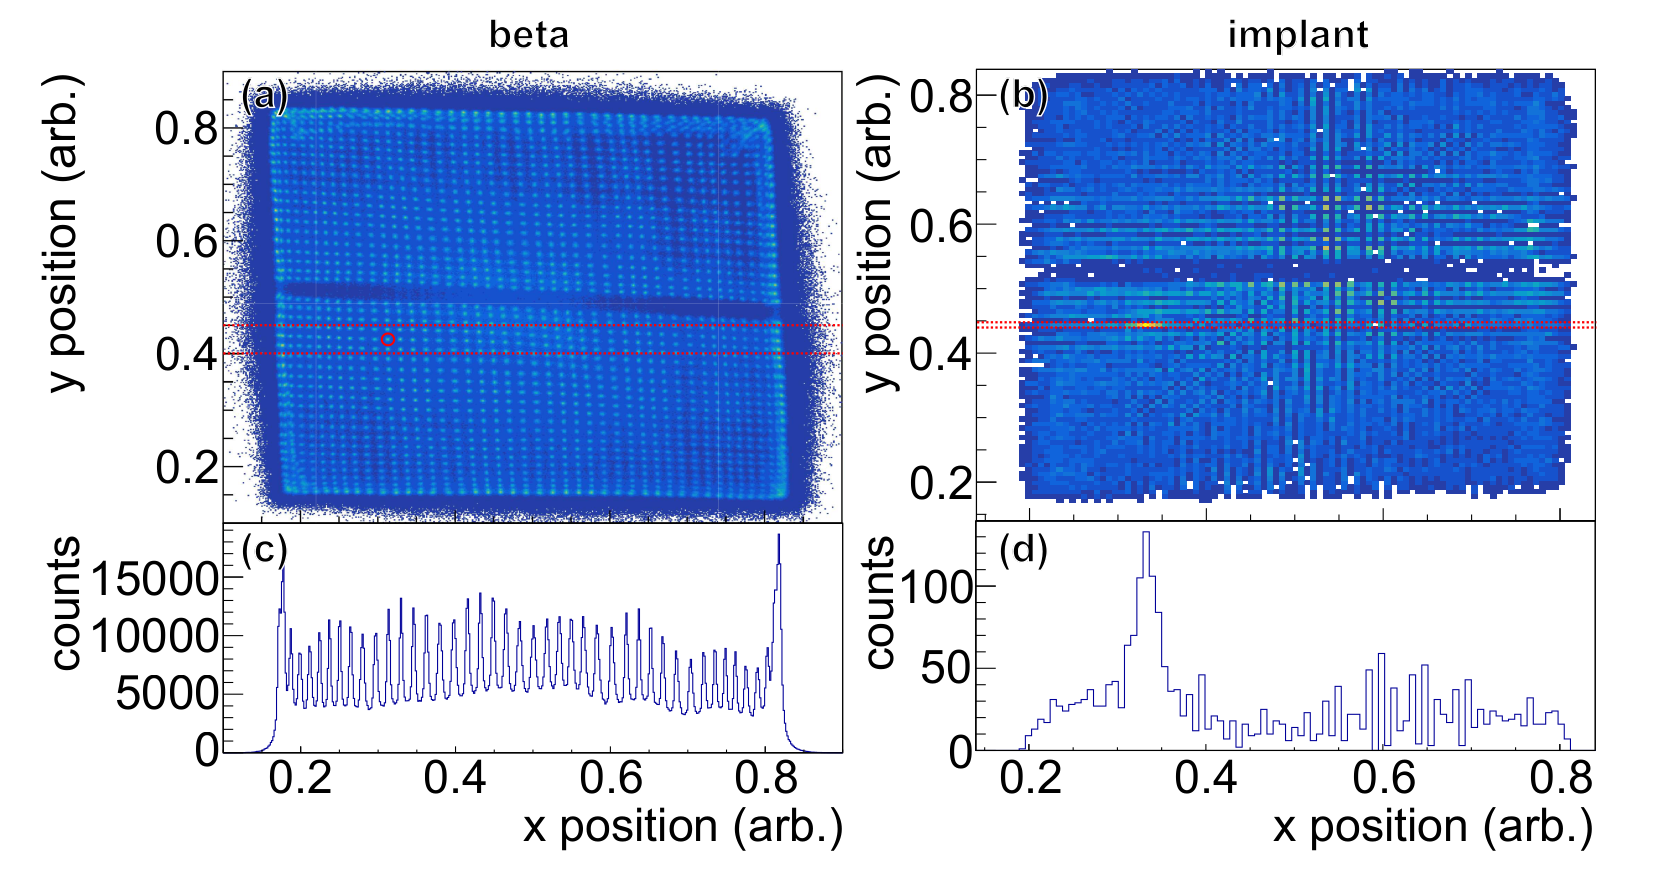
\includegraphics[width=17cm,height=8cm]{figures/ion_beta_correlations.png}
    \caption[YSO x-y images of (a) $\beta$ events and (b) implantation events correlated]{YSO x-y images of (a) $\beta$ events and (b) implantation events correlated to the $\beta$ events in a segment shown in the red circle in panel (a). (c) and (d) are the projection of (a) and (b), respectively, on to the x axis in the cut shown by the red dashed lines \citep{yso2018}.}
\label{fig:ysocorrelations}
\end{figure}

\newpage
\begin{figure}[h!]
    \centering
    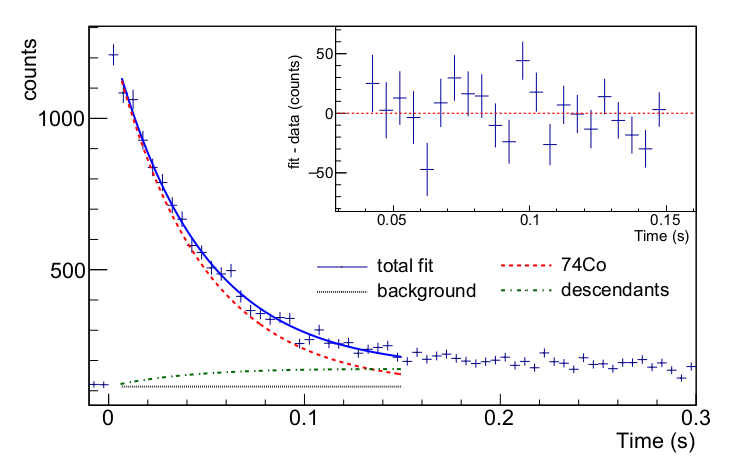
\includegraphics[width=15cm,height=10cm]{figures/half_life.png}
    \caption[The decay curve of the $\beta$ rays from \textsuperscript{74}Co decays]{The decay curve of the $\beta$ rays from \textsuperscript{74}Co decays. The solid blue curve represents the fitting function. The dashed red curve shows the decay component of the parent nucleus,
\textsuperscript{74}Co. The dashed-dotted green curve is the sum of the daughter and neutron-daughter branches. The dotted black line shows the linear background. The plot at the right top of the
figure shows the difference between the data points and the
fitting function \citep{yso2018}.}
    \label{fig:yso_halflife}
\end{figure}

\pagebreak

\section{Delayed Neutron Emission Spectroscopy using \textbf{VANDLE} at RIBF, RIKEN}
Versatile Array of Neutron Detectors at Low Energy (VANDLE) comprises a set of elongated neutron detectors capable of detecting neutrons having the energy of the order of MeV. The individual detector is made up of Eljen-EJ200 organic scintillator bar, coupled to PMT on both sides to collect the light produced. Based on the dimension of the scintillator used, the individual detectors are classified small, medium, and large. VANDLE offers good timing and spatial resolution \citep{VANDLE} for measuring neutrons. For the experiment, a set of 48 medium ($3 \times$ 6 $\times$ 180 $cm^{3}$) arranged in a semi-circular fashion with a diameter 210 cm was implemented. Two high purity germanium clovers and a total of 10 LaBr\textsubscript{3} detectors were placed around YSO to capture decay based $\gamma$-excitations. Signals from all the detectors were read-out using digital electronics modules called Pixie-16 \citep{PIXIE16} by XIA. Each of the modules has 16 channels with four Field Programmable Gate Arrays (FPGA), and a fast built-in Analog to Digital Conversion (ADC) at the rate of 250 Mega samples per second. The experiment took place at RIBF factory at RIKEN Nishina Center, Japan in December 2018. The experiments involved accelerating \textsuperscript{238}U upto 345 MeV/nucleon with a charge state of (86+) which is the primary beam, followed by hitting a 4 mm thick rotating target of \textsuperscript{9}Be, with primay beam intensity peaking $\sim$ 45 pnA. The in-beam fission fragments were selected to be in and around the vicinity of \textsuperscript{78}Ni by the BigRIPS \citep{FUKUDA2013323} facility. The whole experimental campaign lasted for about 5.5 days. The data looks promising, and a great deal of new physics about the structural arrangement and evolution of nuclei in the \textsuperscript{78}Ni region is anticipated from the analysis.

\begin{figure}[h]
    \centering
    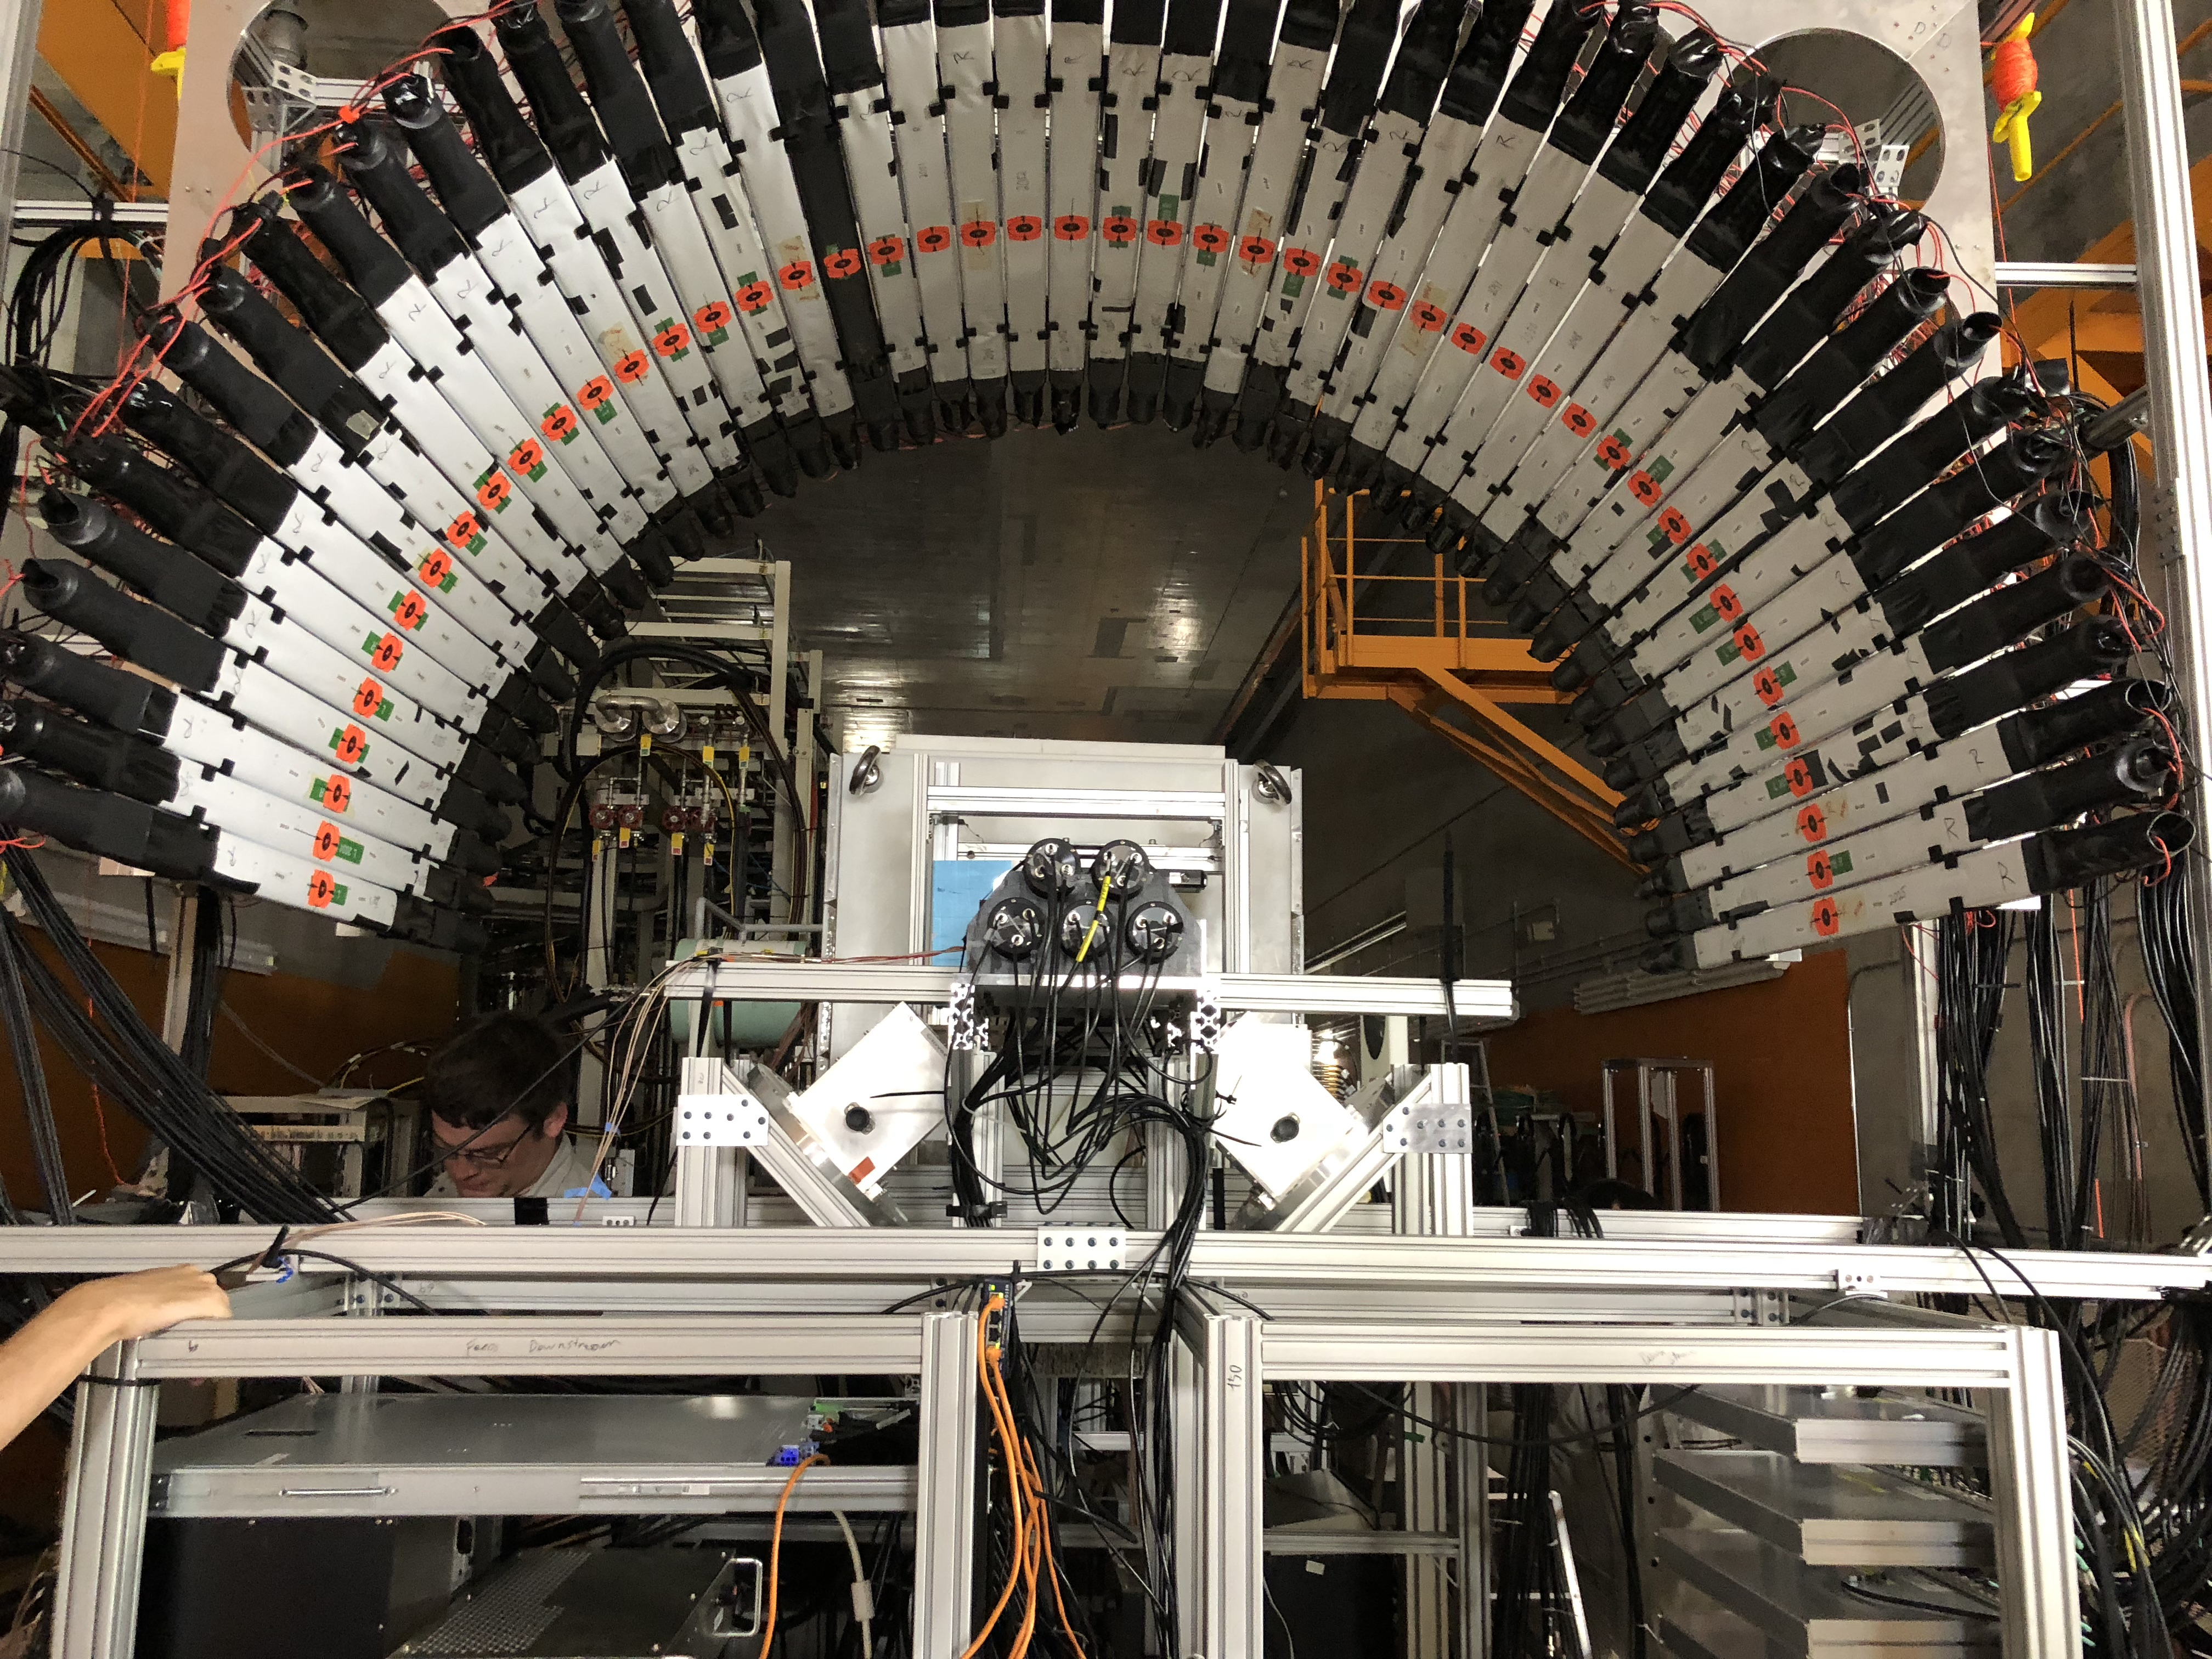
\includegraphics[width=12cm,height=10cm]{figures/vandle_ribf.jpg}
    \caption[The picture shows the site of the experimental setup]{The picture shows the site of the experimental setup at RIBF, RIKEN for the experiment employing VANDLE. The setup was further downstream the F11 focal plane. The setup consists 48 VANDLE bars, YSO (70 $\times$ 70 $\times$ 5  mm\textsuperscript{3}), two high purity germanium clover detectors setup at 90 degrees angle to each other, and 10 LaBr\textsubscript{3} detectors.}
    \label{fig:vandleribf}
\end{figure}


\begin{figure}[h]
	\centering
	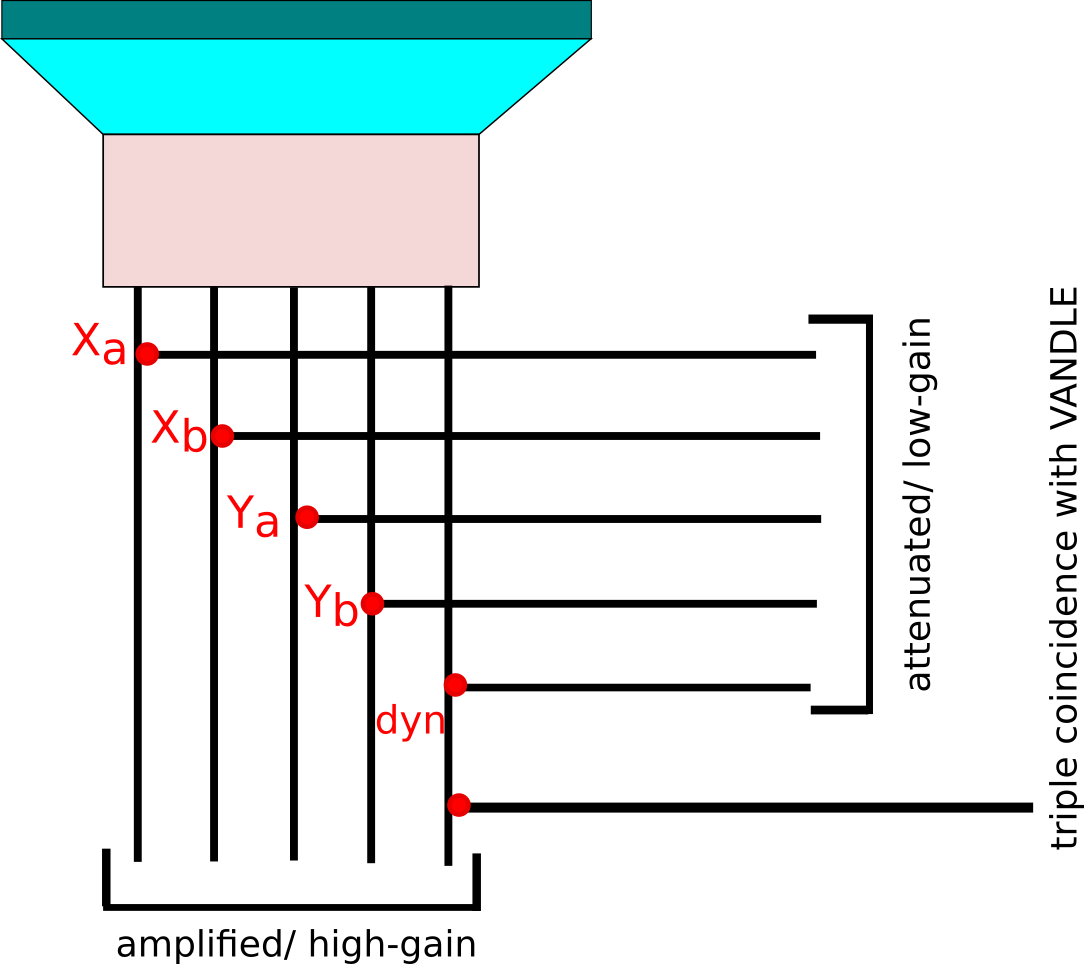
\includegraphics[width=14cm, height=10cm]{figures/YSO_trigger_scheme.png}
	\caption[Division of the 5 YSO signals into low- and high-gain branches]{Division of the 5 YSO signals into low- and high-gain branches. A red dot denote a split in the signal.}
	\label{fig:ysotriggervandle}
\end{figure}

\begin{figure}[h]
    \centering
    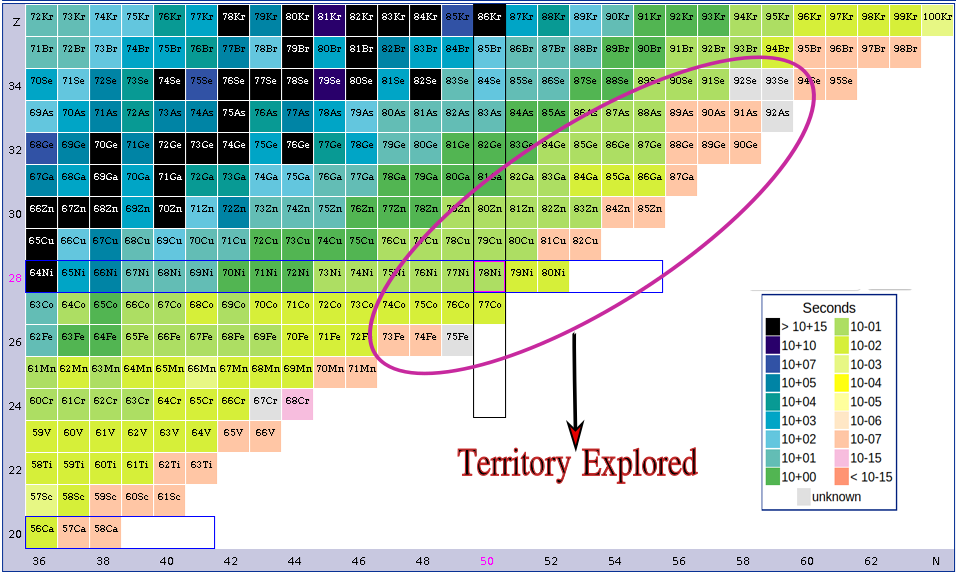
\includegraphics[width=10cm, height=8cm]{figures/nuclie_chart_plot.png}
    \caption[The figure displays a zoomed-in section of nuclei chart]{The figure displays a zoomed in section of nuclei chart, showing the region explored in the experiment, demarcated by a red ellipse.}
    \label{fig:chart_nuclie}
\end{figure}

Provide a block diagram of the setup and explain each component.explain HagRID detectors and what are they made up of. 



\subsection{Trigger Scheme for the experiment}

    \chapter{Analysis} \label{ch:analysis}

The following chapter contains the analysis techniques used  as well as developed for analysis from the following experiments:



\section{BRIKEN experiment}

\subsection{YSO }
\subsection{Ion-beta correlations}
\subsection{Calibrations of low- and high-gain branches}


\section{VANDLE experiment}
\subsection{Particle identification}

As mentioned in the experiment section, particle identification is performed by the BigRIPS particle separator using the TOF-B$\rho$-$\Delta$E method. The values of \textit{Z} and \textit{A/Q} are deduced using the measured values of TOF, B$\rho$, and $\Delta$E using the following equations:

The time of flight of a particle for a flight path L:

\begin{equation}\label{eq:1}
TOF = \frac{L}{\beta c}
\end{equation}

Equating Lorentz and centripetal forces experienced by a particle in magnetic field B:

\begin{equation}\label{eq:2}
\frac{A}{Q} = \frac{B \rho}{\beta \gamma} \frac{c}{m_{u}}
\end{equation}


The Bethe-bloch formula describing energy-loss ($\Delta$E) of a particle a material:

\begin{equation}\label{eq:3}
\frac{dE}{dx}=\frac{4\pi e^{4}Z^{2}}{m_{e} \nu^{2}} Nz \Bigg[ ln \frac{2m_{e} \nu^{2}}{I} -ln(1-\beta^2) -\beta^{2}\Bigg],
\end{equation}


Here $\beta=\nu/c$, $\gamma = 1/ \sqrt{1-\beta^2}$) is the velocity of the particle, $m_{u}$ = 931.4 MeV is the atomic mass unit, $m_{e}$ is the electron mass, and e is the electron charge. z, N and I represent the atomic number, atomic density and mean excitation of the material, respectively. $\textit{Z, A}$ and \textit{Q} denote the proton number, atomic mass, and charge states of a fragment, respectively.


move the Bigrips picture here:

Now from the diagram of the BigRIPS separator we can see that the flight path L is from F3 to F7, and is measured by thin plastic scintillators located at F3 and F7. The foci at F3 and F7 are fully achromatic, while the ones at F1 and F5 are momentum dispersive. $\Delta$E is measured by using the multi-sampling ionization chamber (MUSIC) located at F7. The $B \rho$ measurement is done using the trajectory reconstruction from F3-F5 and from F5-F7. The trajectory of the particles is tracked with the help of a position-sensitive parallel plate avalanche counters (PPAC) located at F3, F5, and F7. 

The PPAC detectors and the energy degrader at F5 lead to energy loss. Hence, $B \rho$ measurements are done for F3-F5 path and F5-F7 path. The leads to a change in equations \ref{eq:1} and \ref{eq:2} as follows:

\begin{equation} \label{eq:4}
TOF = \frac{L_{35}}{\beta c_{35}} + \frac{L_{57}}{\beta c_{57}}
\end{equation}


\begin{equation}\label{eq:5}
\left (\frac{A}{Q} \right)_{35} = \frac{B \rho_{35}}{\beta_{35} \gamma_{35}} \frac{c}{m_{u}}
\end{equation}


\begin{equation}\label{eq:6}
\left (\frac{A}{Q} \right)_{57} = \frac{B \rho_{57}}{\beta_{57} \gamma_{57}} \frac{c}{m_{u}}
\end{equation}


If the charge state of the ion does not change on its course from F3 to F7 at F5. We will have the following relation by equating \ref{eq:5} and \ref{eq:6}: 


\begin{equation}\label{eq:7}
\frac{B \rho_{35}}{B \rho_{57}} = \frac{\beta_{35} \gamma_{35}}{\beta_{57} \gamma_{57}}
\end{equation}


The velocities of the fragments before and after F5 can be deduced using equations \ref{eq:4} and \ref{eq:7} from the measured TOF and $B\rho_{35,57}$ values. The absolute value of $\textit{Z}$ can be then deduced using by modifying equation \ref{eq:3} as follows:

\begin{equation}\label{eq:8}
Z = a \beta \sqrt{\frac{\Delta E}{ln \left (\frac{2m_{e} c^2 \beta^2}{I} \right ) -ln(1-\beta^2) -\beta^{2}}} + b
\end{equation}

where the inputs to the equation are $\Delta E$ and $\beta_{57}$, a and b are the parameters that need to be determined during the experiment from calibrations.

In the follwoing sections we show the cuts and gates implemented in the data for building cleaner events tagged with calibrated \textit{Z} and \textit{A/Q}.


\subsubsection{F3 and F7}

Plastic scintillator detectors located at F3 and F7 for measuring TOF are readout using the photomultplier tubes (PMT), which are coupled to the left and right ends of the detector. The position of an incident particle can be found using the charge-integrated signals $q_{1}$ and $q_{2}$ from left and right end of the detector using the following expression:

\begin{equation}\label{eq:9}
x = -\dfrac{\lambda}{2} ln \left ( \dfrac{q_{1}}{q{2}} \right ).
\end{equation}


Here, $\lambda$ denotes the attenuation length of scintillation light in the detector. We can also get the position from the timing of the left and right PMT siganls as 

\begin{equation}\label{eq:10}
x = -\dfrac{V}{2}(t_{2}-t_{1})
\end{equation}

By equating Eqs \ref{eq:9} and \ref{eq:10} we got the basis for rejecting signals in the data lying far-off from the constraint defined by the following equation:

\begin{equation}\label{eq:11}
-\dfrac{\lambda}{2} ln \left ( \dfrac{q_{1}}{q{2}} \right ) = \dfrac{V}{2}(t_{2}-t_{1})
\end{equation}

where V denotes the propagation speed of light in the scintillation counter. Figure \ref{fig:F3_plastic_cut} and \ref{fig:F7_plastic_cut} shoes the correlation derived from time-difference and the ratio of the left and right PMT signal amplitudes from the data.

\begin{figure}[h]
	\centering
	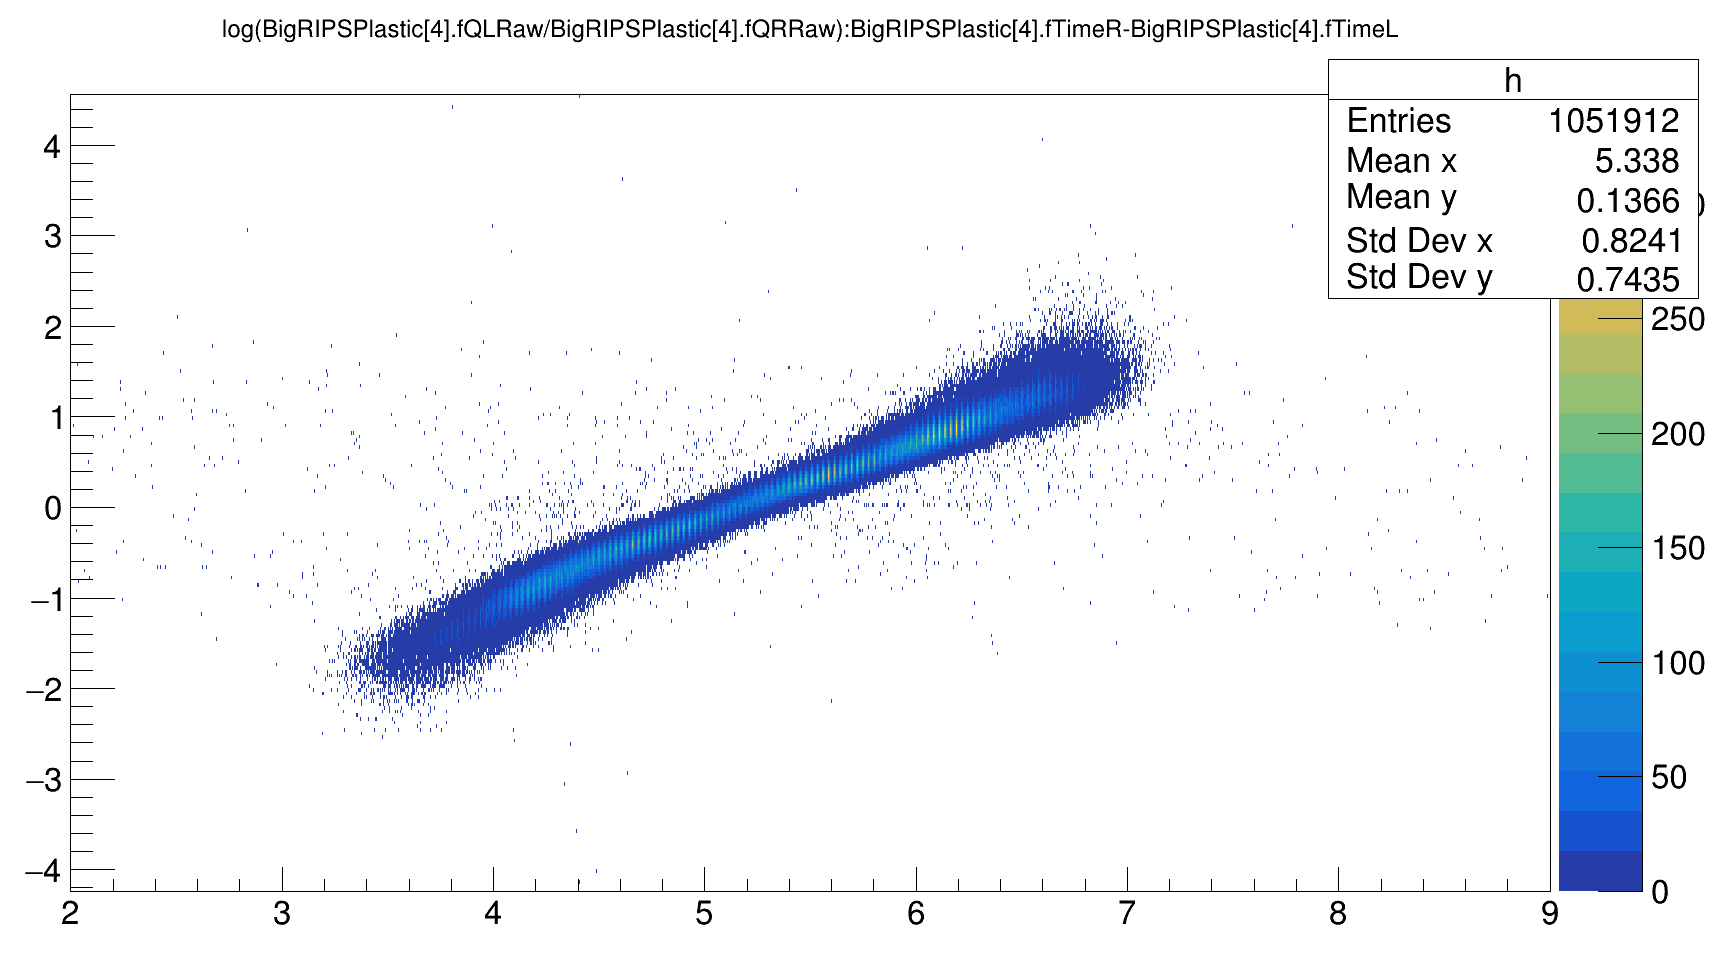
\includegraphics[width=6cm,height=4cm]{figures/F3_plastic_cut.png}
	\caption[Implementation of cuts at F3 plastic to reject background events.]{Implementation of cuts at F3 and F7 plastic to reject background events.}
	\label{fig:F3_plastic_cut}
\end{figure}

\begin{figure}[h]
	\centering
	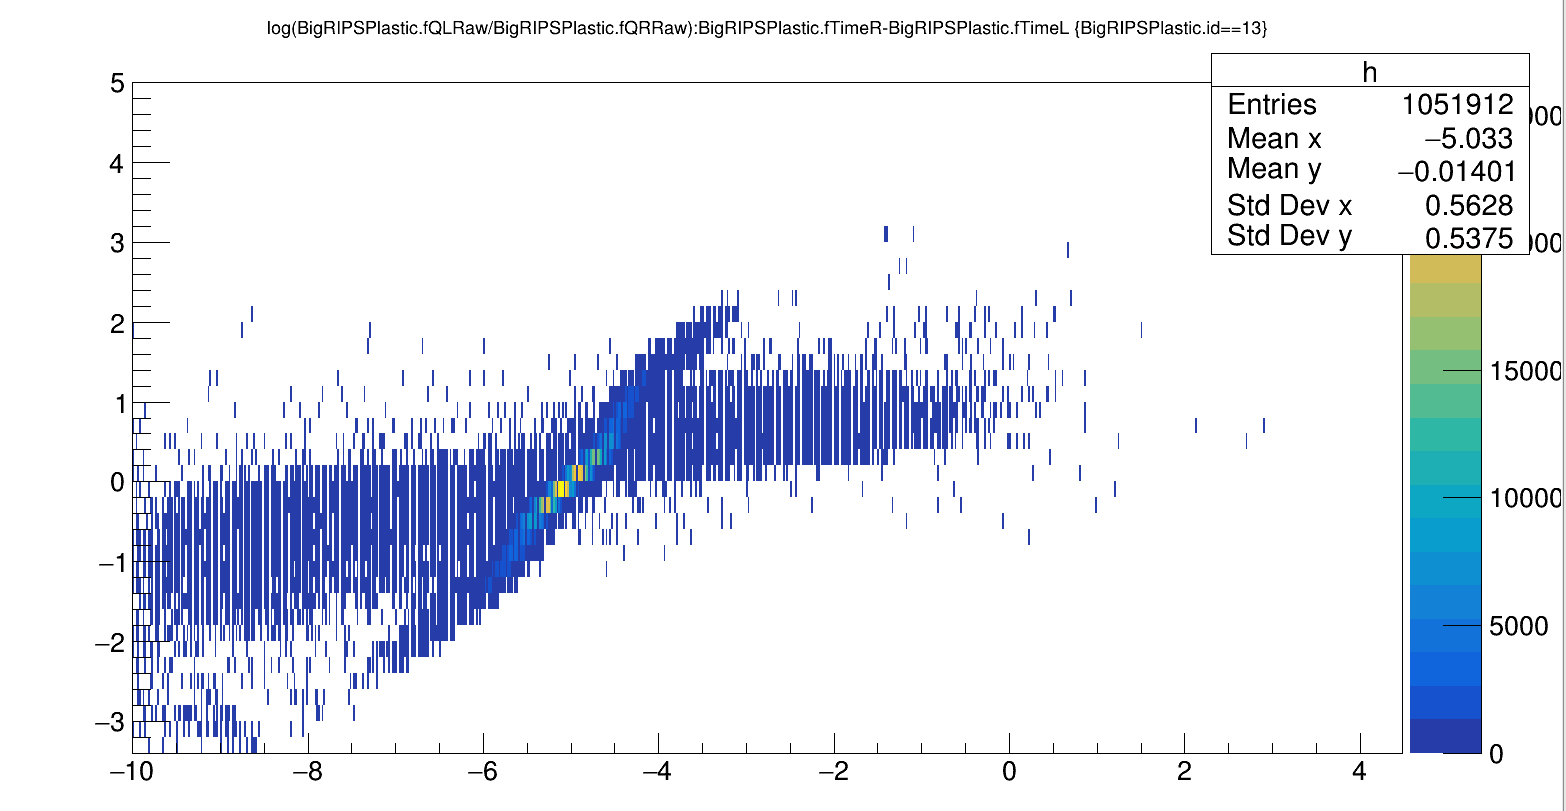
\includegraphics[width=6cm,height=4cm]{figures/F7_plastic_cut.png}
	\caption[Implementation of cuts at F7 plastic to reject background events.]{Implementation of cuts at F3 and F7 plastic to reject background events.}
	\label{fig:F7_plastic_cut}
\end{figure}

\subsubsection{PPAC}

The position-sensitive Parallel Plate Avalance Counter (PPAC) are used for tracking the fragments in the beamline at RIBF. The detector consist of several plates with 4 readouts ($T_{X_{(1, 2)}}$ and $T_{Y_{(1, 2)}}$) for position tracking. The detectors adopt a delay-line readout method [N FUKUDA]. The position of an incident particle is determined from the time difference between two timing signals $T_{1}$ and $T_{2}$ obtained from the ends of the delay line in the PPAC detector. The sum of the timing defined as 


\begin{equation}
T_{sum} = T_{1} + T_{2},
\end{equation}

remains constant independent of the position of the incident particle, and acts as an important tool to remove inconsistent events and effects of $\delta$-rays from the data.

\begin{figure}[h]
	\centering
	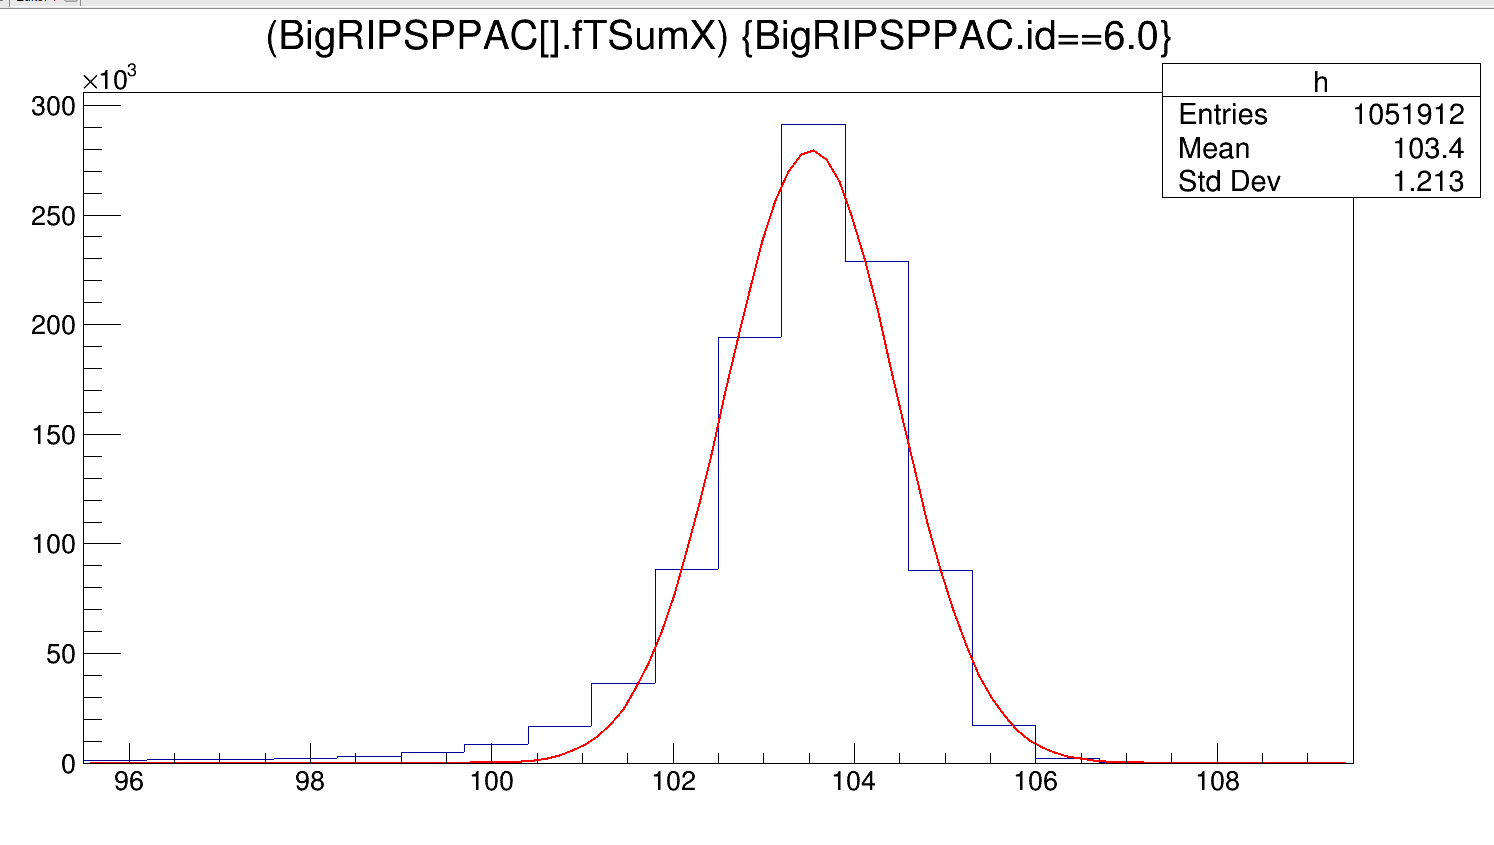
\includegraphics[width=8cm,height=6cm]{figures/PPAC_cut.png}
	\caption[]{$T_{sum}$ for the sum of one of the plates of PPAC at F3. Only events lying within the FWHM range of the main peak are accepted. }
	\label{fig:PPAC_cut}
\end{figure}

As an example, Figure \ref{fig:PPAC_cut} shows the $T_{sum}$ distribution for \textit{X} position signals of one of the plates of PPAC located at F3. Similar cuts were used for all the PPAC detector plates in the BigRIPS separator.

 
 
\subsubsection{MUSIC ($\Delta$E) detector}

The MUSIC detector used for the $\Delta$E measurement in the BigRIPS separator consists of twelve anodes and thirteen cathodes aligned alternately. The neighboring anodes are electrically connected in pairs. The six anode signals are read independently and averaged for the $\Delta$E measurement. The fragments on their way through the MUSIC detector can cause nuclear reactions with the electrodes and the counter gas. The correlation between alternative anodes helps to remove inconsistent events from the beam. 

\begin{figure}[h]
	\centering
	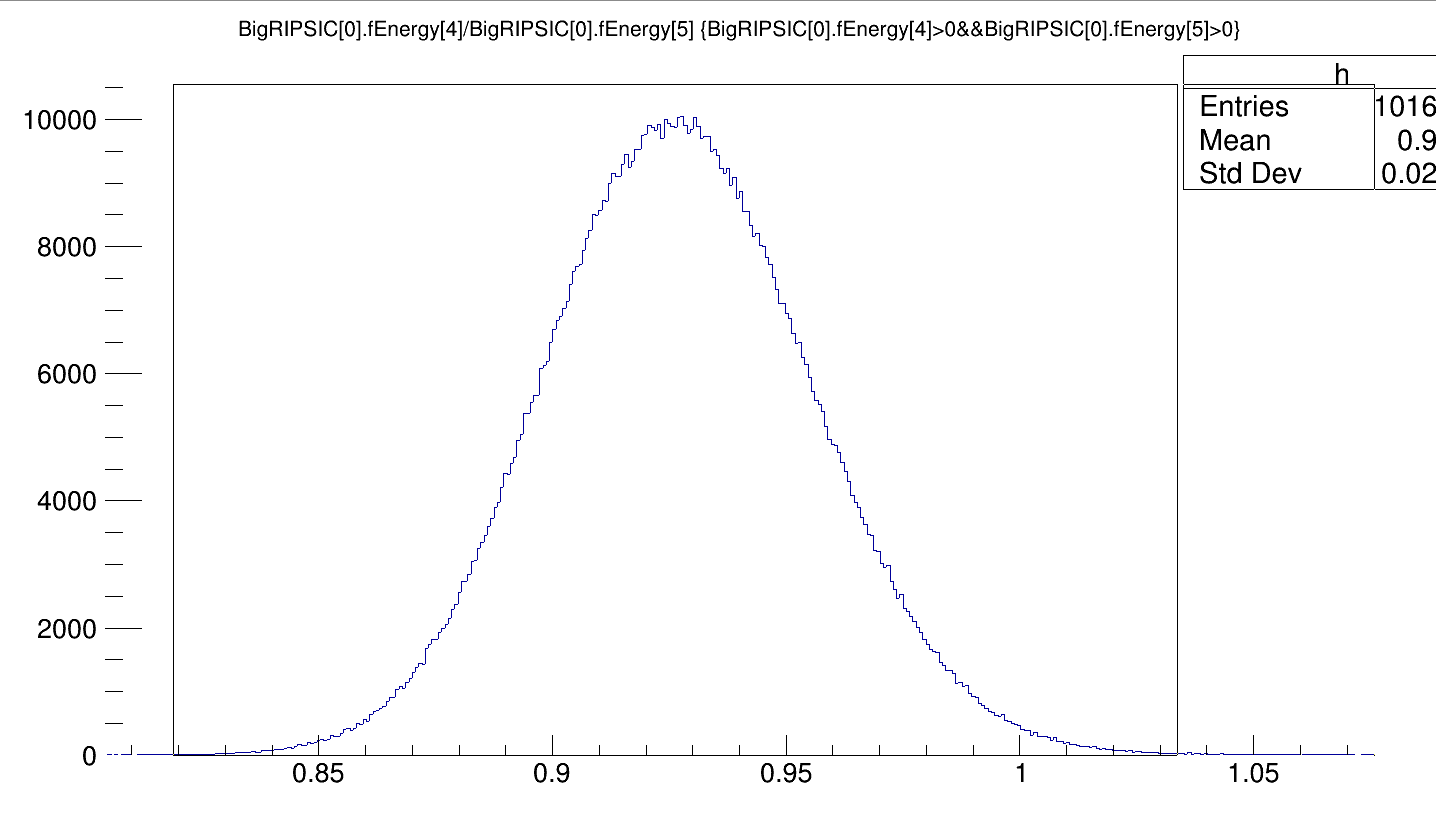
\includegraphics[width=10cm,height=6cm]{figures/MUSIC_detector.png}
	\caption[]{Ratio of 5th and 4th anode signal for the MUSIC detector.}
	\label{fig:MUSIC_cut}
\end{figure}

As an example, Figure \ref{fig:MUSIC_cut} shows the ratio of signals from two consecutive anodes. The signals were accepted within the FHWM of the peak of the distribution. Similar gates were implemented for all the consecutive anode signals.

\begin{figure}[h]
	\centering
	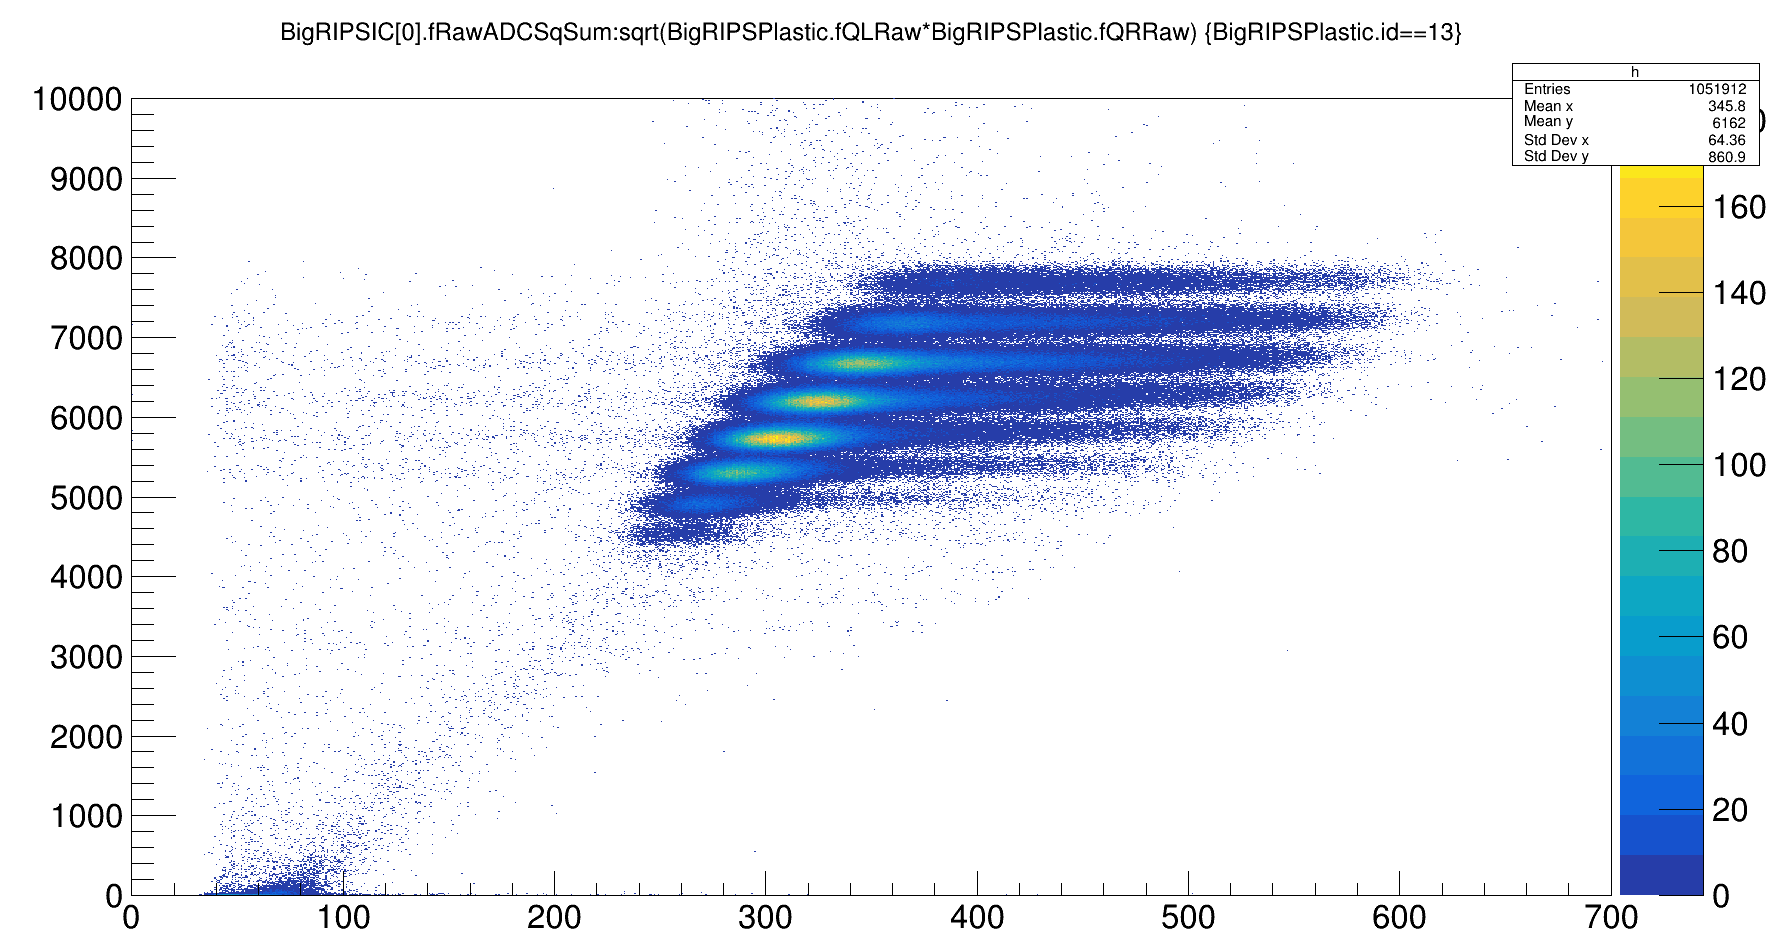
\includegraphics[width=10cm,height=6cm]{figures/F7_MUSIC.png}
	\caption[]{}
	\label{fig:F7_MUSIC}
\end{figure}

Further, fragments upon leaving F7 plastic can have a change in the charge state due to reactions in the F7 plastic. These events were rejected using correlation between the signal from the MUSIC detector and the signals from the left and right of the F7 plastic as shown in Figure \ref{fig:F7_MUSIC}.




The source of noise in data was identified to be in the F7 plastic as shown in Figure \ref{fig:F7_Plastic}. Upon the implementation of all these a liner function for calibration of \textit{Z} used. 


\begin{figure}[h]
	\centering
	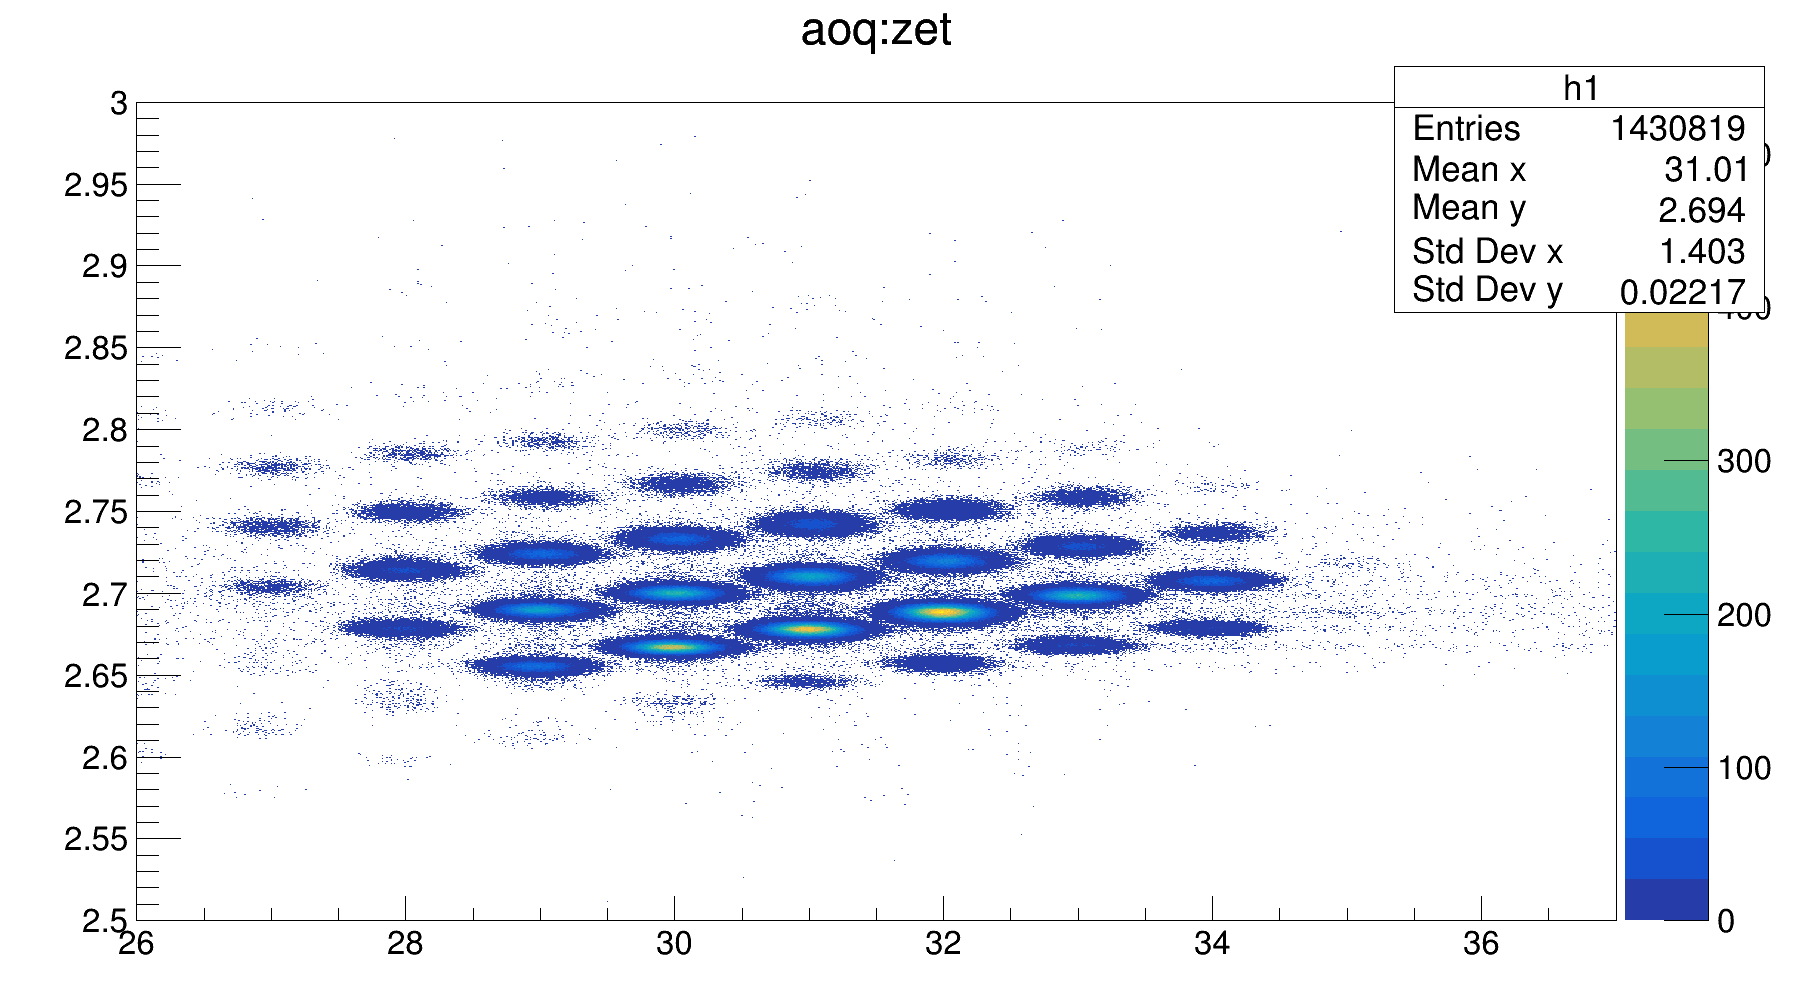
\includegraphics[width=10cm,height=6cm]{figures/PID_uncleaned.png}
	\caption[]{}
	\label{fig:PID_uncleaned_F7}
\end{figure}


\begin{figure}[h]
	\centering
	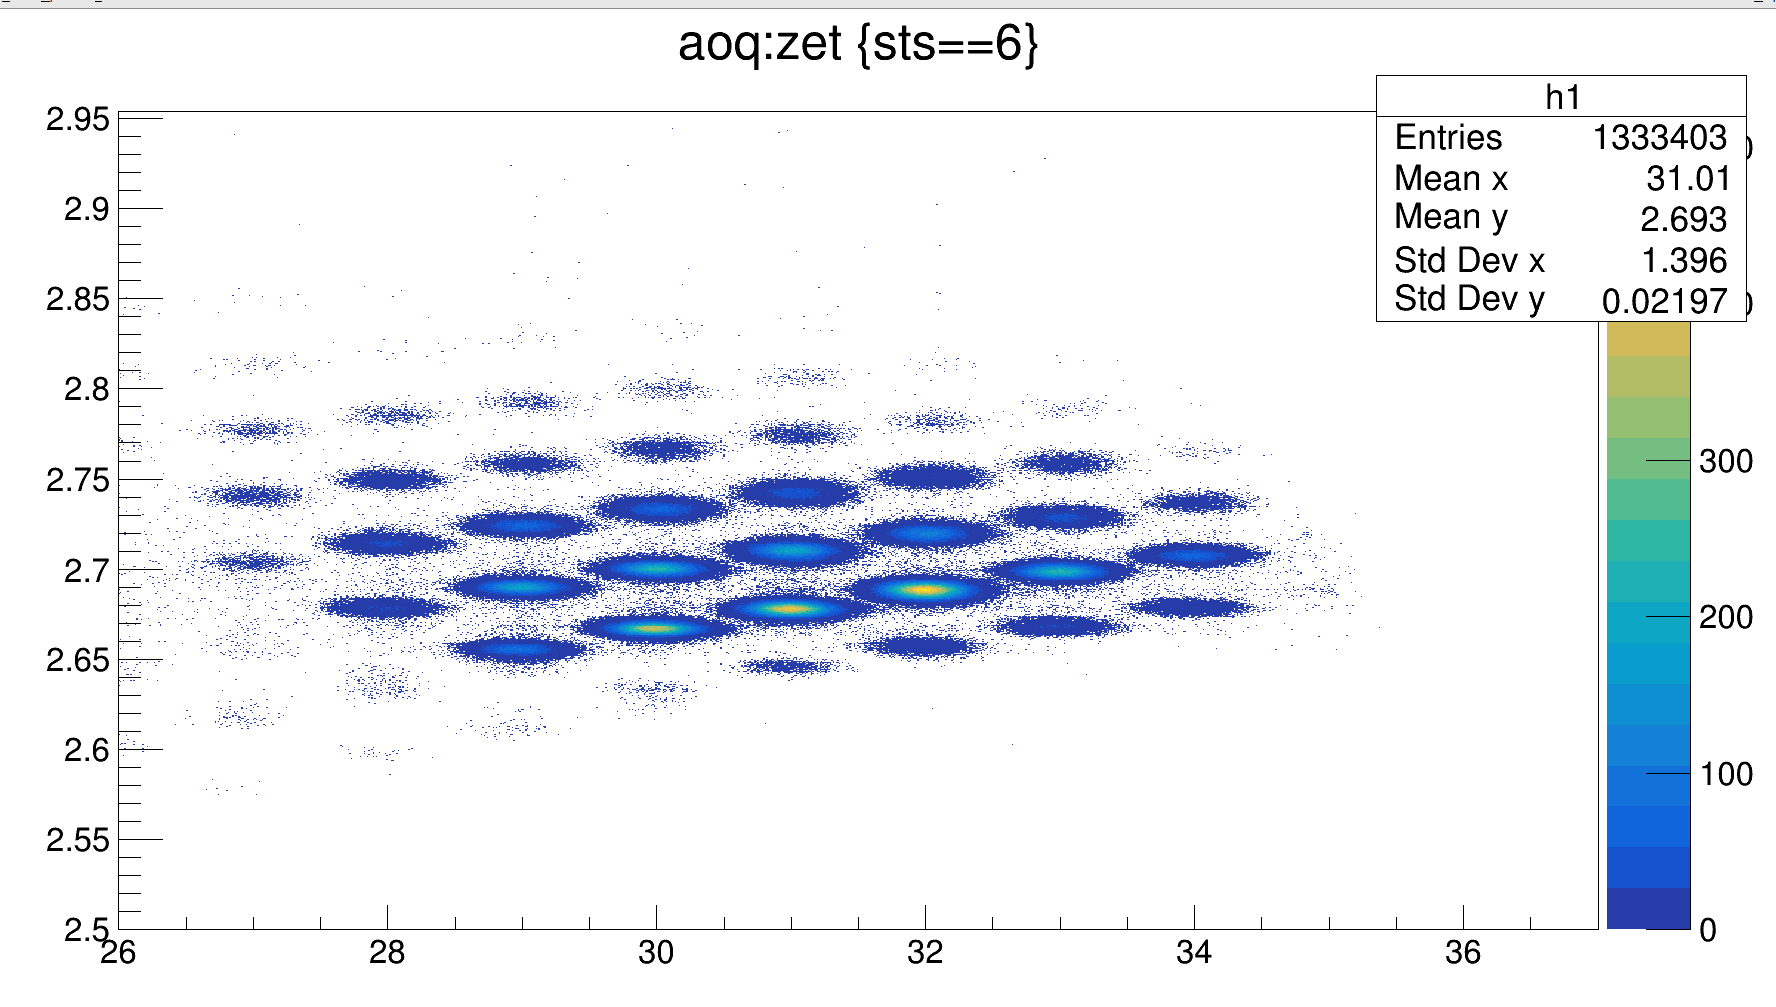
\includegraphics[width=10cm,height=6cm]{figures/PID_cleaned.png}
	\caption[]{}
	\label{fig:PID_cleaned_F7}
\end{figure}

\newpage

\section{Clovers}

The main analysis for clovers constituted of calibration and efficiency calculations. A clover detector contains 4 HPGe crystals sensitive to $\gamma$-rays. The crystals need to be calibrated individually followed by proper gain-matching to get a good resolution. For efficiency and calibration data were collected using standard sources in the experiment configuration. Calibrated sources, such as $\textsuperscript{133}$Ba, $\textsuperscript{60}$Co, $\textsuperscript{137}$Cs, and $\textsuperscript{152}$Eu were used for efficiency measurements. Some of the crystals of the clovers suffered from gain shift during the experiment. Thus, calibration parameters from the source run could not be implemented for the experiment runs. However, a number of known background lines were identified in the in-beam runs and they were used for calibration. The lines are listed below along with their sources.

/*VERIFY from the cheat sheet in the office*/
\begin{center}
	\begin{tabular}{ |c|c|c| } 
		\hline
		$\gamma$-ray (keV) & Source \\
		\hline
		351.9 & $\textsuperscript{214}Pb(Ra)$ \\ 
		511 & Pair production \\ 
		788.7 & $\textsuperscript{138}La$ \\ 
		1435.7 & $\textsuperscript{138}La$ \\ 
		1460.8 & $\textsuperscript{40}K$ \\ 
		1764.5 & $\textsuperscript{214}Bi(Ra)$ \\ 
		2614.7 & $\textsuperscript{208}Tl(Th)$ \\ 
		\hline
	\end{tabular}
\end{center}

A polynomial of first order as shown in equation \ref{eq:clover_calibration} was used to calibrate clover spectrum to keV.
\begin{equation} \label{eq:clover_calibration}
E_{\gamma} = a*E_{ch} + b
\end{equation}
Here, a and b represent the calibration parameters.



The YSO detector is sensitive to $\gamma$-rays and acts a $\gamma$-ray absorber. Hence, this can lead to a lowering of $\gamma$-ray efficiency, more adversely for low-energy $\gamma$-rays. To properly account for the absorption effects from the YSO and for the sake of accuracy, efficiency for clovers was measured by placing a standard source for the mentioned list at different position on the face of the YSO detector. Figure \ref{fig:YSO_source_holder} shows the layout the source holder and this source holder was affixed onto the face of the YSO detector to quantify change in the efficiency with a change in the position of a gamma source in the YSO detector.

\begin{figure}[h]
	\centering
	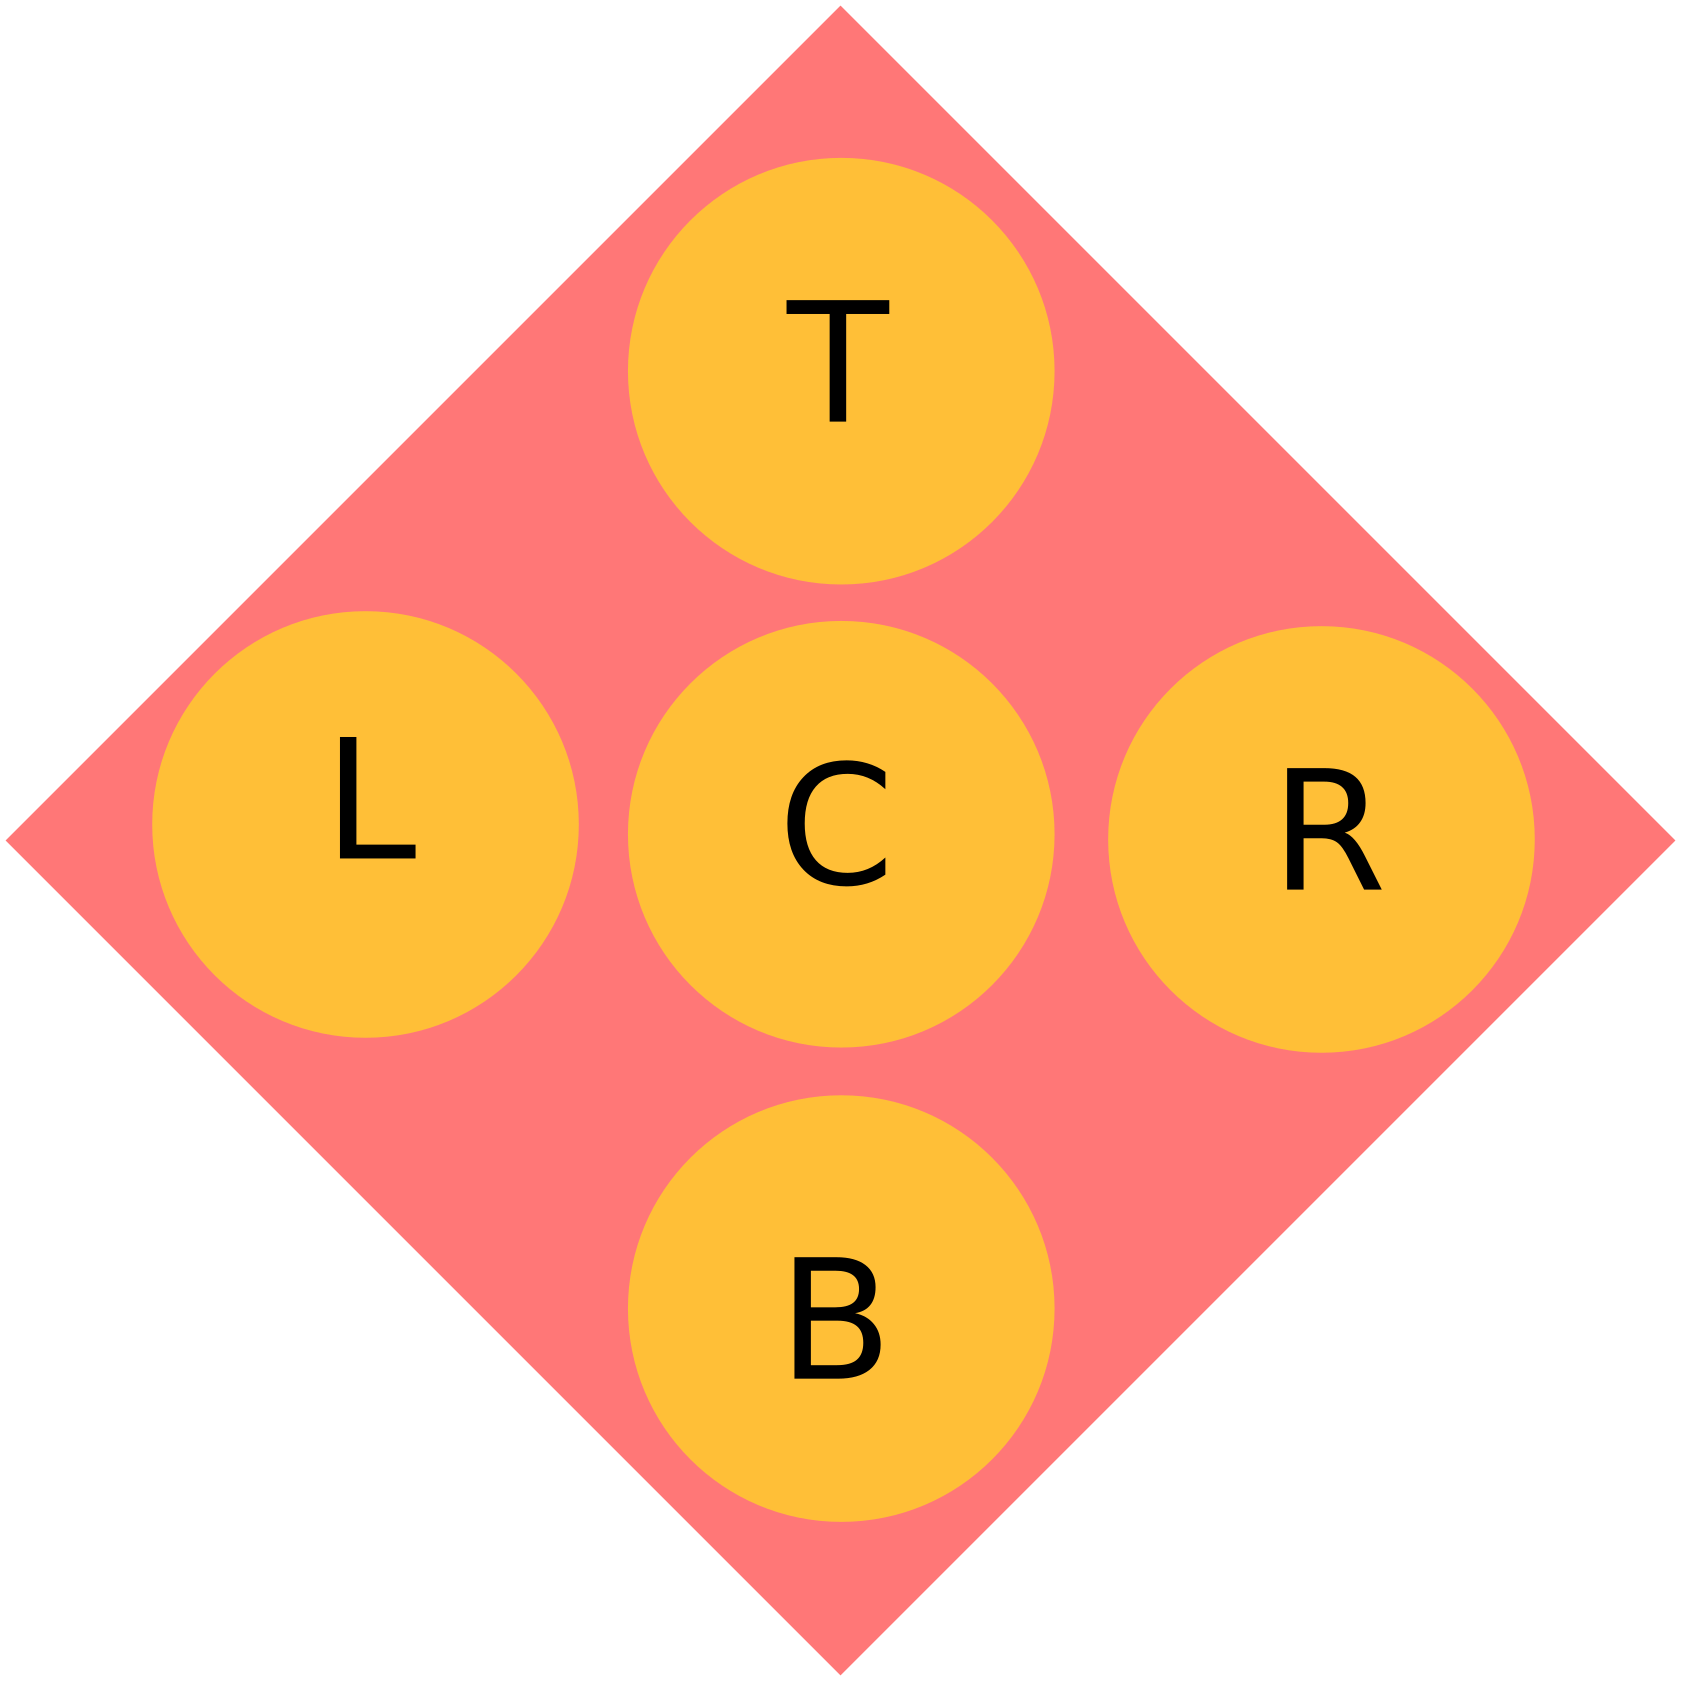
\includegraphics[scale=0.5]{figures/Yso_source_holder.png}
	\caption[]{Design of a 3D-printed source holder matching the dimensions of the YSO. Yellow circles show cavities for placing a source. The source positions are labeled as top (T), bottom (B), left (L), right(R), and center (C). }
	\label{fig:YSO_source_holder}
\end{figure}


Further, from the efficiency measurements it was seen that the data from $\textsuperscript{152}Eu$ was subjected to significant dead time due to high source activity. The dead time then leads to a underestimation of the efficiency. The dead time was calculated using count rate for 1435.7-keV line from $\textsuperscript{138}La$. The ratio of the count rate from the background and the source data gives the required scaling needed for the main peaks in the source run.Figure \ref{fig:1435_7_background} shows the dead time for all the source runs. $\textsuperscript{152}Eu$ suffers from most of the dead time. The same count rate was calculated for in-beam runs,and it showed no dead time.

\begin{figure}[h]
	\centering
	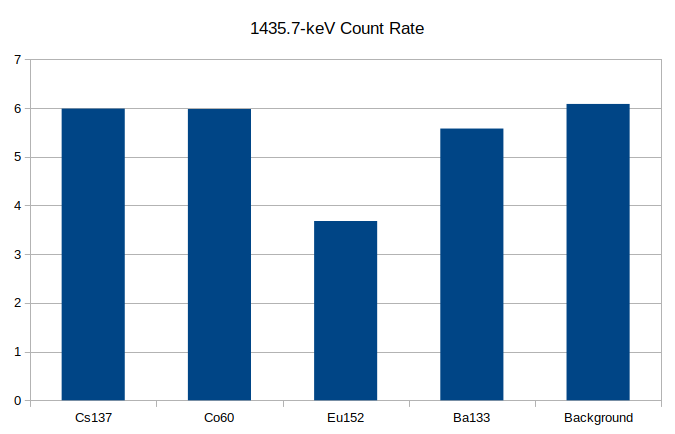
\includegraphics[scale=0.5]{figures/background_count_rate.png}
	\caption[]{Dead time across all the source runs.}
	\label{fig:1435_7_background}
\end{figure}


The data collected for the efficiency measurements was later used to benchmark a GEANT4 simulation package. The 
benchmark here is to get a reliable efficiency measurements from the GEANT4 when a source is place at any position on the face of the YSO detector. The criterion adopted for the benchmark  was to have efficiency from the simulations within the error bars at each for measurements at each of the positions or there is a discrepancy no more than $\sim$ 5-8 $\%$ between the data and the simulations. Also, a number a simulations were run to find a position for the center of the YSO crystal relative to the clovers in the simulation software setup to meet the criterion.

\begin{figure}[h]
	\centering
	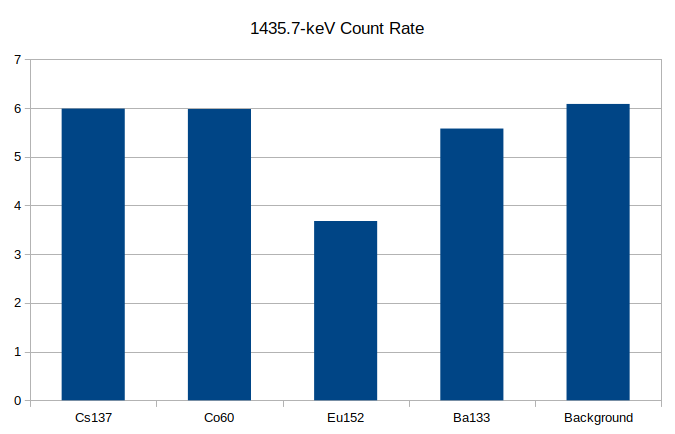
\includegraphics[scale=0.5]{figures/background_count_rate.png}
	\caption[]{Dead time across all the source runs.}
	\label{fig:1435_7_background}
\end{figure}









	
	


\*Mention explicitly all the algorithms used for the analysis*\
\subsection{Data Streams Merging}
\subsection{YSO Analysis Development}
\subsection {Dynamic Range Tests}
\subsubsection{Reconstruction of ion and beta distributions}
\subsection{Comparison of Gates showing background and dynode-single energy curve}
\subsection{Properties of the PSPMT, Vertilon Board and the light guide used}
\subsection{Put electronics diagrams of both the PSPMT and the board, elaborate the working in a reductive manner; split the paragraphs before}
\subsection{Development of algorithm for ion-beta correlations}
\subsubsection{Beta Background Quantify}
\subsection{Bateman equation fitting for Cu80}
\subsection{Explanation for counting betas for the beta delayed neutron emitters using the bateman equations}
\subsection{Bateman equation fitting for Ga83}
explain the shape of the decay curve 
\subsection{VANDLE Analysis}
\subsubsection{Efficiency Measurements}
\subsection{Americium Measurement}
\subsection{Time Calibration}
\subsection{Walk Characteristics}
\subsubsection {Walk Correction for YSO and VANDLE}
Explain the methodology as you filled in the sheet.
\subsection{Flight Path Reconstruction using implant position coordinates}
\subsection{Cu81 neutron spectrum}

Analysis will include preparation of ion-beta timing gate

\subsection{Cu80 neutron spectrum}
\subsection{Cu79 neutron spectrum}




Plot graphs with the ratios of the timing corrected and uncorrected to gauge the position of YSO.

Talk about the technique to find the offset.

\subsection{Neutron Background Subtraction Techniques}
\subsection{Neutron Calibration}
\subsection{YSO light quenching Estimates}

Explain the process for the YSO light quenching
Calibration
low-gain branch calibration in MeVee
quenching factors for various isotopes 
Lise++ plots showing kinetic energy distribution

\section{Gamma-ray Analysis}
\subsubsection{Addback}
\subsubsection{Efficiency characterization using GEANT4}
Main points would be describe the characterization of the efficiency/bench-marking.
Technique developed to get efficiency estimates using implant position and using gamma efficiency on an event-by-event basis. 
\subsubsection{HaGRID}

\section{GEANT4 simulations}

\subsection{VANDLE efficiency from simulations}

\subsection{Explain the estimates of efficiency}
\subsection{Explain the bench-marking process for the simulation}
\subsubsection{Gain Adjustment of the VANDLE PMT}
\subsubsection{Response Function development}

discuss the anatomy and the shape of the function. Discuss the shape of the function and the reflection from the top of the function.
\subsection{Estimates for the threshold using data for single bar}
\subsection{}

\subsection{Need for simulations}
Explain with respect to understanding the scattering and affects from various components from the decay station. Need to extract the response

Explain the affect of the YSO in the setup

Import the pictures for scattering positions for the ions in the setup.

Give details of the response function and its anatomy used in the analysis.

Show the fitting of the function for a particular case

Write the equations for various parameters

plot the qdc ratio to extract position using scatter positions


\section{Analysis of \textsuperscript{81,80,79}Cu}
\subsection{Ion-beta correlation}
\subsection{Beta-gated Gamma-ray spectrum}
\subsection{Neutron-gamma Coincidence}
Go in step wise order for the whole data analysis.
Give a general overview of the decay for the whole isotope.

(graphics use DNP 2020 Cu81 as an example.)

Explain the need and how it helps assigning strength for all excited energy levels.
\subsection{De-convolution of neutron spectrum}
Show the histogram here and the calculated peaks.

\subsection{BGT formation}
calculations
\section{discussions}

Write about the results of the analysis
\section{}

    \chapter{Results} \label{ch:results}
    
    %%%%%%%%%%%%%%%%%%%%%%%%%%%%%%%%%%%%%%%%%%%%%%%%%%%%%%%%%%%%%%%%%%%%%%%%%%%%%%%%%%%%%%%%%%%%%%%%%%%%%
    % BIBLIOGRAPHY
    %%%%%%%%%%%%%%%%%%%%%%%%%%%%%%%%%%%%%%%%%%%%%%%%%%%%%%%%%%%%%%%%%%%%%%%%%%%%%%%%%%%%%%%%%%%%%%%%%%%%%
    \makeBibliographyPage % make the bibliography title page
    \bibliographystyle{unsrt}
\newpage

% To make the bibliography, use \utbiblio{#1}{}{} command. Always use "#1" for the first entry. The second entry is your bibliography style, and the third entry is the name of your bibliography file (.bib file extension) 
% bibliography style - recommend using apalike-doi as it hyperlinks DOIs
% Be sure to run BibTeX in order to generate the bibliography correctly.

\utbiblio{#1}{apalike}{references-dissertation}

    %%%%%%%%%%%%%%%%%%%%%%%%%%%%%%%%%%%%%%%%%%%%%%%%%%%%%%%%%%%%%%%%%%%%%%%%%%%%%%%%%%%%%%%%%%%%%%%%%%%%%
    % APPENDIX - OPTIONAL - COMMENT OUT IF NOT NEEDED
    %%%%%%%%%%%%%%%%%%%%%%%%%%%%%%%%%%%%%%%%%%%%%%%%%%%%%%%%%%%%%%%%%%%%%%%%%%%%%%%%%%%%%%%%%%%%%%%%%%%%%
    
    \makeAppendixPage{2}   % Input the number of appendices
    \appendix    
    
\section{Summary of Equations}
some text here
\subsection{Cartesian}
some equations here

\subsection{Cylindrical}
some equations also here
    
\section{Summary of Stuff}
some text here
\subsection{More Things}
some equations here

\subsection{Other Aspects}
some equations also here

    %%%%%%%%%%%%%%%%%%%%%%%%%%%%%%%%%%%%%%%%%%%%%%%%%%%%%%%%%%%%%%%%%%%%%%%%%%%%%%%%%%%%%%%%%%%%%%%%%%%%%
    % A VITA IS REQUIRED
    %%%%%%%%%%%%%%%%%%%%%%%%%%%%%%%%%%%%%%%%%%%%%%%%%%%%%%%%%%%%%%%%%%%%%%%%%%%%%%%%%%%%%%%%%%%%%%%%%%%%%
    \addToTOC{Vita}
    \chapter*{Vita} \label{ch:vita}
Vita goes here. The vita should be a brief biography about the author written in third person and paragraph format. It should not be the author's resume or CV.
\end{document}
